% Options for packages loaded elsewhere
\PassOptionsToPackage{unicode}{hyperref}
\PassOptionsToPackage{hyphens}{url}
%
\documentclass[
]{article}
\usepackage{amsmath,amssymb}
\usepackage{lmodern}
\usepackage{iftex}
\ifPDFTeX
  \usepackage[T1]{fontenc}
  \usepackage[utf8]{inputenc}
  \usepackage{textcomp} % provide euro and other symbols
\else % if luatex or xetex
  \usepackage{unicode-math}
  \defaultfontfeatures{Scale=MatchLowercase}
  \defaultfontfeatures[\rmfamily]{Ligatures=TeX,Scale=1}
\fi
% Use upquote if available, for straight quotes in verbatim environments
\IfFileExists{upquote.sty}{\usepackage{upquote}}{}
\IfFileExists{microtype.sty}{% use microtype if available
  \usepackage[]{microtype}
  \UseMicrotypeSet[protrusion]{basicmath} % disable protrusion for tt fonts
}{}
\makeatletter
\@ifundefined{KOMAClassName}{% if non-KOMA class
  \IfFileExists{parskip.sty}{%
    \usepackage{parskip}
  }{% else
    \setlength{\parindent}{0pt}
    \setlength{\parskip}{6pt plus 2pt minus 1pt}}
}{% if KOMA class
  \KOMAoptions{parskip=half}}
\makeatother
\usepackage{xcolor}
\IfFileExists{xurl.sty}{\usepackage{xurl}}{} % add URL line breaks if available
\IfFileExists{bookmark.sty}{\usepackage{bookmark}}{\usepackage{hyperref}}
\hypersetup{
  pdftitle={Day 2},
  pdfauthor={Solveig Bjørkholt},
  hidelinks,
  pdfcreator={LaTeX via pandoc}}
\urlstyle{same} % disable monospaced font for URLs
\usepackage[margin=1in]{geometry}
\usepackage{color}
\usepackage{fancyvrb}
\newcommand{\VerbBar}{|}
\newcommand{\VERB}{\Verb[commandchars=\\\{\}]}
\DefineVerbatimEnvironment{Highlighting}{Verbatim}{commandchars=\\\{\}}
% Add ',fontsize=\small' for more characters per line
\usepackage{framed}
\definecolor{shadecolor}{RGB}{248,248,248}
\newenvironment{Shaded}{\begin{snugshade}}{\end{snugshade}}
\newcommand{\AlertTok}[1]{\textcolor[rgb]{0.94,0.16,0.16}{#1}}
\newcommand{\AnnotationTok}[1]{\textcolor[rgb]{0.56,0.35,0.01}{\textbf{\textit{#1}}}}
\newcommand{\AttributeTok}[1]{\textcolor[rgb]{0.77,0.63,0.00}{#1}}
\newcommand{\BaseNTok}[1]{\textcolor[rgb]{0.00,0.00,0.81}{#1}}
\newcommand{\BuiltInTok}[1]{#1}
\newcommand{\CharTok}[1]{\textcolor[rgb]{0.31,0.60,0.02}{#1}}
\newcommand{\CommentTok}[1]{\textcolor[rgb]{0.56,0.35,0.01}{\textit{#1}}}
\newcommand{\CommentVarTok}[1]{\textcolor[rgb]{0.56,0.35,0.01}{\textbf{\textit{#1}}}}
\newcommand{\ConstantTok}[1]{\textcolor[rgb]{0.00,0.00,0.00}{#1}}
\newcommand{\ControlFlowTok}[1]{\textcolor[rgb]{0.13,0.29,0.53}{\textbf{#1}}}
\newcommand{\DataTypeTok}[1]{\textcolor[rgb]{0.13,0.29,0.53}{#1}}
\newcommand{\DecValTok}[1]{\textcolor[rgb]{0.00,0.00,0.81}{#1}}
\newcommand{\DocumentationTok}[1]{\textcolor[rgb]{0.56,0.35,0.01}{\textbf{\textit{#1}}}}
\newcommand{\ErrorTok}[1]{\textcolor[rgb]{0.64,0.00,0.00}{\textbf{#1}}}
\newcommand{\ExtensionTok}[1]{#1}
\newcommand{\FloatTok}[1]{\textcolor[rgb]{0.00,0.00,0.81}{#1}}
\newcommand{\FunctionTok}[1]{\textcolor[rgb]{0.00,0.00,0.00}{#1}}
\newcommand{\ImportTok}[1]{#1}
\newcommand{\InformationTok}[1]{\textcolor[rgb]{0.56,0.35,0.01}{\textbf{\textit{#1}}}}
\newcommand{\KeywordTok}[1]{\textcolor[rgb]{0.13,0.29,0.53}{\textbf{#1}}}
\newcommand{\NormalTok}[1]{#1}
\newcommand{\OperatorTok}[1]{\textcolor[rgb]{0.81,0.36,0.00}{\textbf{#1}}}
\newcommand{\OtherTok}[1]{\textcolor[rgb]{0.56,0.35,0.01}{#1}}
\newcommand{\PreprocessorTok}[1]{\textcolor[rgb]{0.56,0.35,0.01}{\textit{#1}}}
\newcommand{\RegionMarkerTok}[1]{#1}
\newcommand{\SpecialCharTok}[1]{\textcolor[rgb]{0.00,0.00,0.00}{#1}}
\newcommand{\SpecialStringTok}[1]{\textcolor[rgb]{0.31,0.60,0.02}{#1}}
\newcommand{\StringTok}[1]{\textcolor[rgb]{0.31,0.60,0.02}{#1}}
\newcommand{\VariableTok}[1]{\textcolor[rgb]{0.00,0.00,0.00}{#1}}
\newcommand{\VerbatimStringTok}[1]{\textcolor[rgb]{0.31,0.60,0.02}{#1}}
\newcommand{\WarningTok}[1]{\textcolor[rgb]{0.56,0.35,0.01}{\textbf{\textit{#1}}}}
\usepackage{longtable,booktabs,array}
\usepackage{calc} % for calculating minipage widths
% Correct order of tables after \paragraph or \subparagraph
\usepackage{etoolbox}
\makeatletter
\patchcmd\longtable{\par}{\if@noskipsec\mbox{}\fi\par}{}{}
\makeatother
% Allow footnotes in longtable head/foot
\IfFileExists{footnotehyper.sty}{\usepackage{footnotehyper}}{\usepackage{footnote}}
\makesavenoteenv{longtable}
\usepackage{graphicx}
\makeatletter
\def\maxwidth{\ifdim\Gin@nat@width>\linewidth\linewidth\else\Gin@nat@width\fi}
\def\maxheight{\ifdim\Gin@nat@height>\textheight\textheight\else\Gin@nat@height\fi}
\makeatother
% Scale images if necessary, so that they will not overflow the page
% margins by default, and it is still possible to overwrite the defaults
% using explicit options in \includegraphics[width, height, ...]{}
\setkeys{Gin}{width=\maxwidth,height=\maxheight,keepaspectratio}
% Set default figure placement to htbp
\makeatletter
\def\fps@figure{htbp}
\makeatother
\setlength{\emergencystretch}{3em} % prevent overfull lines
\providecommand{\tightlist}{%
  \setlength{\itemsep}{0pt}\setlength{\parskip}{0pt}}
\setcounter{secnumdepth}{-\maxdimen} % remove section numbering
\usepackage{float}
\ifLuaTeX
  \usepackage{selnolig}  % disable illegal ligatures
\fi

\title{Day 2}
\usepackage{etoolbox}
\makeatletter
\providecommand{\subtitle}[1]{% add subtitle to \maketitle
  \apptocmd{\@title}{\par {\large #1 \par}}{}{}
}
\makeatother
\subtitle{Workflow and Github}
\author{Solveig Bjørkholt}
\date{28. June 2022}

\begin{document}
\maketitle

\hypertarget{plan-for-today}{%
\section{Plan for today}\label{plan-for-today}}

\hypertarget{what-we-will-learn-today}{%
\subsection{What we will learn today:}\label{what-we-will-learn-today}}

\begin{itemize}
\tightlist
\item
  What R and RStudio is.
\item
  Writing and running code.
\item
  Calling functions.
\item
  Introduction to Rmarkdown and Jupyter Notebooks.
\item
  Paths and directories.
\item
  Github
\end{itemize}

\hypertarget{what-we-will-do-today}{%
\subsection{What we will do today:}\label{what-we-will-do-today}}

\begin{itemize}
\tightlist
\item
  Download R and RStudio (if you haven't already).
\item
  Set up a shared repository in Github.
\item
  Work with version control in Github.
\end{itemize}

\hypertarget{what-is-r-and-rstudio}{%
\section{What is R and RStudio?}\label{what-is-r-and-rstudio}}

R is a programming language, along with many other programming
languages. Perhaps you've heard of some of them? Python, Java,
Javascript, PHP, C, C++\ldots{} We use these programming languages to
communicate with the computer. Typically, there are lots of trade-offs
with using one language over another, for example whether you want your
code to be easily readable by a human, or whether it should make the
requests run fast. Also, some programming languages are good for web
development (e.g.~Javascript and PHP), some work great for background
processes (e.g.~C and C++), and some are favorites for mathematics and
statistical computing (e.g.~python and R). We will be focusing on R in
these sessions, though we have a long-term hope of integrating some
python as well.

Learning R is a journey - and a quite frustrating journey at times,
especially if it's the first programming language you learn. So why
bother learning it? Why not just use excel or SPSS or another personal
drag-and-drop favorite? Well\ldots{}

\begin{itemize}
\tightlist
\item
  R is free. It's non-proprietary and requires no license. Down with the
  big corporations, knowledge for all!
\item
  R enhances reproducibility. Anybody can re-run your code to use for
  their own applications, or to replicate your studies.
\item
  R makes it easier to spot errors. Although errors are pain, we would
  rather have an error message early in the process than spotting a
  mistake two days before you think you've finished the project.
\item
  R offers a large and supportive community to help you, both on the web
  and in real life. R-Meetups, RLadies, RStudio conference, you name it.
\end{itemize}

We often say that we ``code in R'', but we ``work in RStudio''. The
reason for this is that R is the machine doing the calculations, while
RStudio is the framework we work within. So if programming was a car,
then R would be the engine and RStudio would be the bodywork.

\hypertarget{installing-r-and-rstudio-adapted-from-louisa-boulaziz}{%
\subsection{Installing R and RStudio (adapted from Louisa
Boulaziz)}\label{installing-r-and-rstudio-adapted-from-louisa-boulaziz}}

\hypertarget{r}{%
\subsubsection{R}\label{r}}

\begin{enumerate}
\def\labelenumi{\arabic{enumi}.}
\tightlist
\item
  Open an internet browser and go to www.r-project.org
\item
  Click the ``download R'' link in the middle of the page under
  ``Getting Started''.
\item
  Select a CRAN location (a mirror site) and click the corresponding
  link. Here you should go to the Norway click on the link.
\item
  Click the ``Download R for Windows'' or the version for your computer.
  Link at the top of the page. If you have an old Mac, you need to read
  the next page carefully.
\item
  Click on the ``install R for the first time'' link at the top of the
  page (Windows). Mac users have to choose the version of R that is
  suitable for their software system. Old Macbook-users need to make
  sure that they click on the link corresponding to their software. If
  you are unsure about your software, click the apple in the left hand
  corner and go to ``about this Mac''. There it will say MacOS followed
  by the name of the software.
\item
  Click ``Download R for Windows'' and save the executable file
  somewhere on your computer. Run the .exe file and follow the
  installation instructions.
\item
  Now that R is installed, you need to download and install RStudio.
\end{enumerate}

\hypertarget{rstudio}{%
\subsubsection{RStudio}\label{rstudio}}

\begin{enumerate}
\def\labelenumi{\arabic{enumi}.}
\tightlist
\item
  Go to www.rstudio.com and click on the ``Download RStudio'' button.
\item
  Click on the ``Download RStudio Desktop''.
\item
  Click on the version recommended for your system, or the latest
  Windows version, and save the executable file. Run the .exe file and
  follow the installation instructions.
\end{enumerate}

\hypertarget{how-rstudio-works}{%
\subsubsection{How RStudio works}\label{how-rstudio-works}}

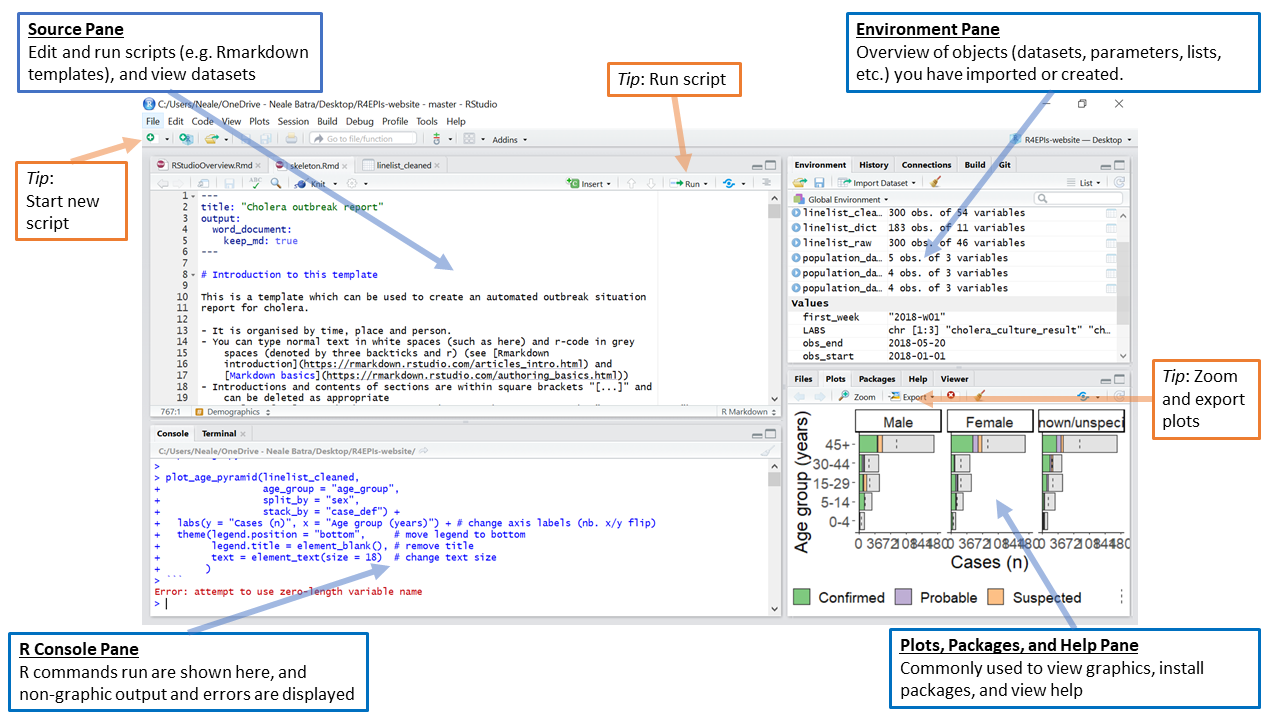
\includegraphics[width=0.8\textwidth,height=\textheight]{./figures/RStudio_overview.png}

\hypertarget{writing-and-running-code}{%
\section{Writing and running code}\label{writing-and-running-code}}

When you have R and RStudio installed, open RStudio. Remember that we
code in R, but work in RStudio, so this is the program you typically
open. Your screen should look something like this:

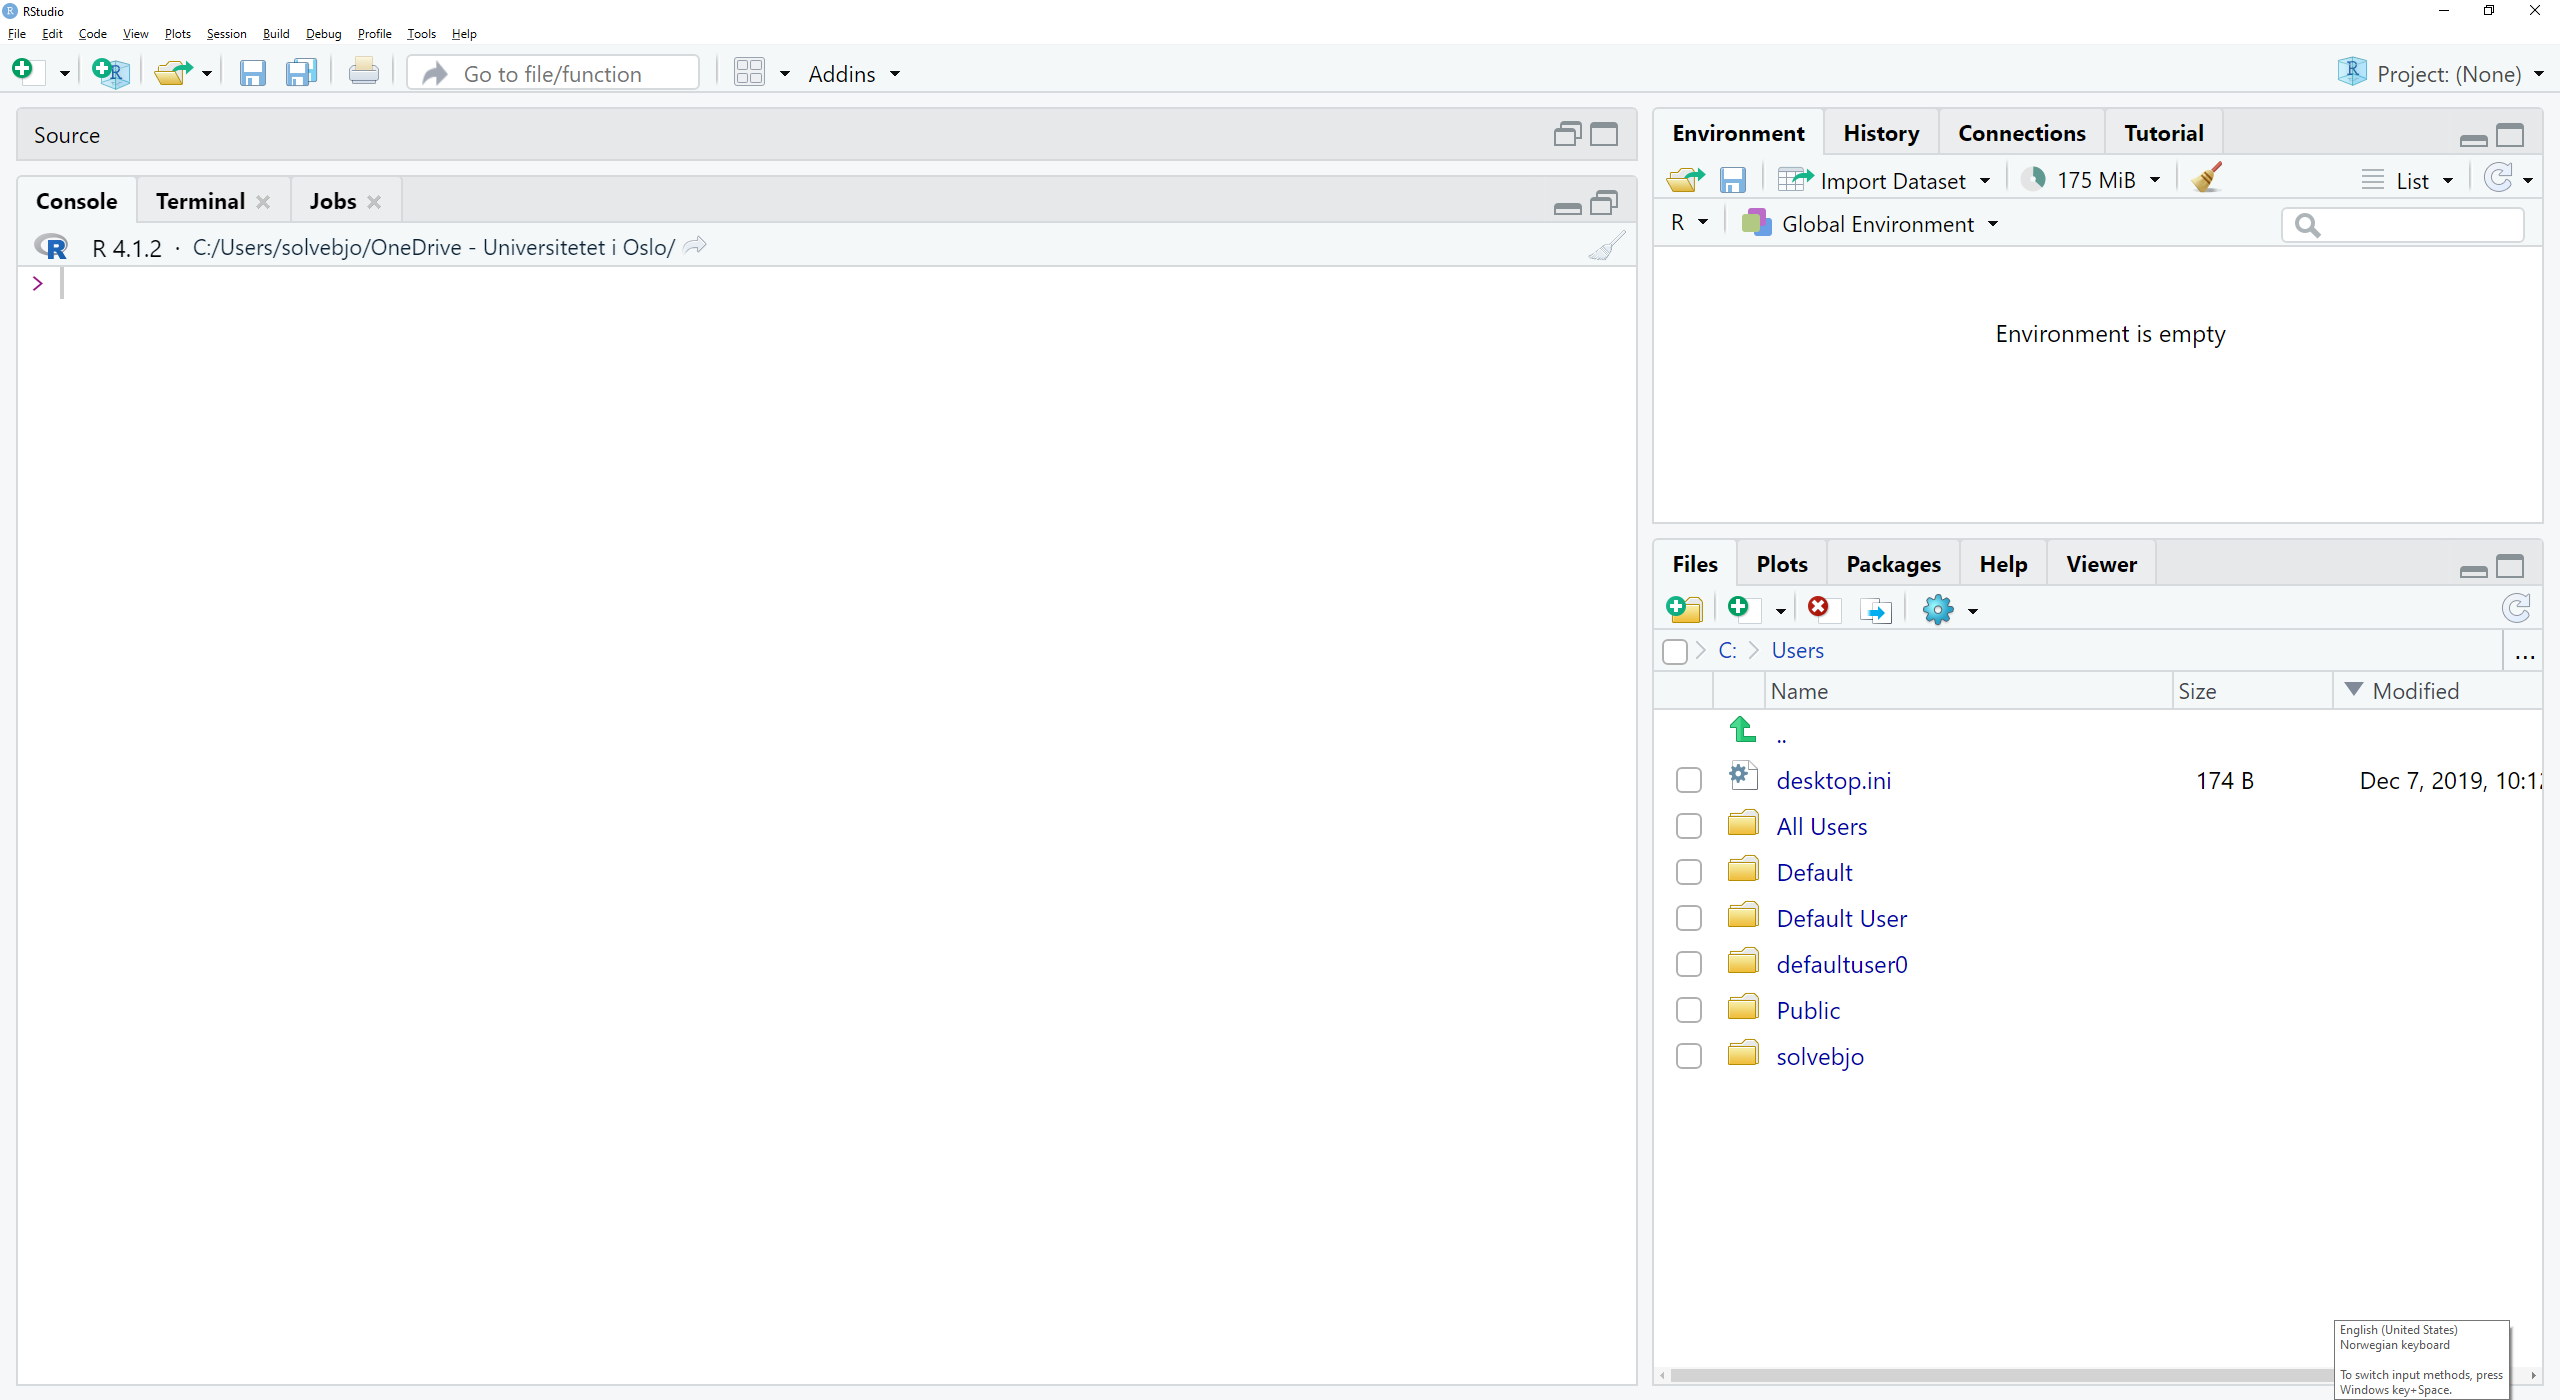
\includegraphics[width=0.8\textwidth,height=\textheight]{./figures/rstudio_1.png}

We want to write our code in a script. A script is kind of like a word
document, just for code. Scripts can be saved, stored and shared with
others, which is preferable to the alternative - to write your code,
execute it and then lose it once you close your programs and go home for
the day. To start a script in RStudio, go to ``File'' and choose ``New
file'', ``R Script''. Alternatively, click on the document with a green
plus-sign in the top left hand corner and choose ``R Script'' - as shown
below.

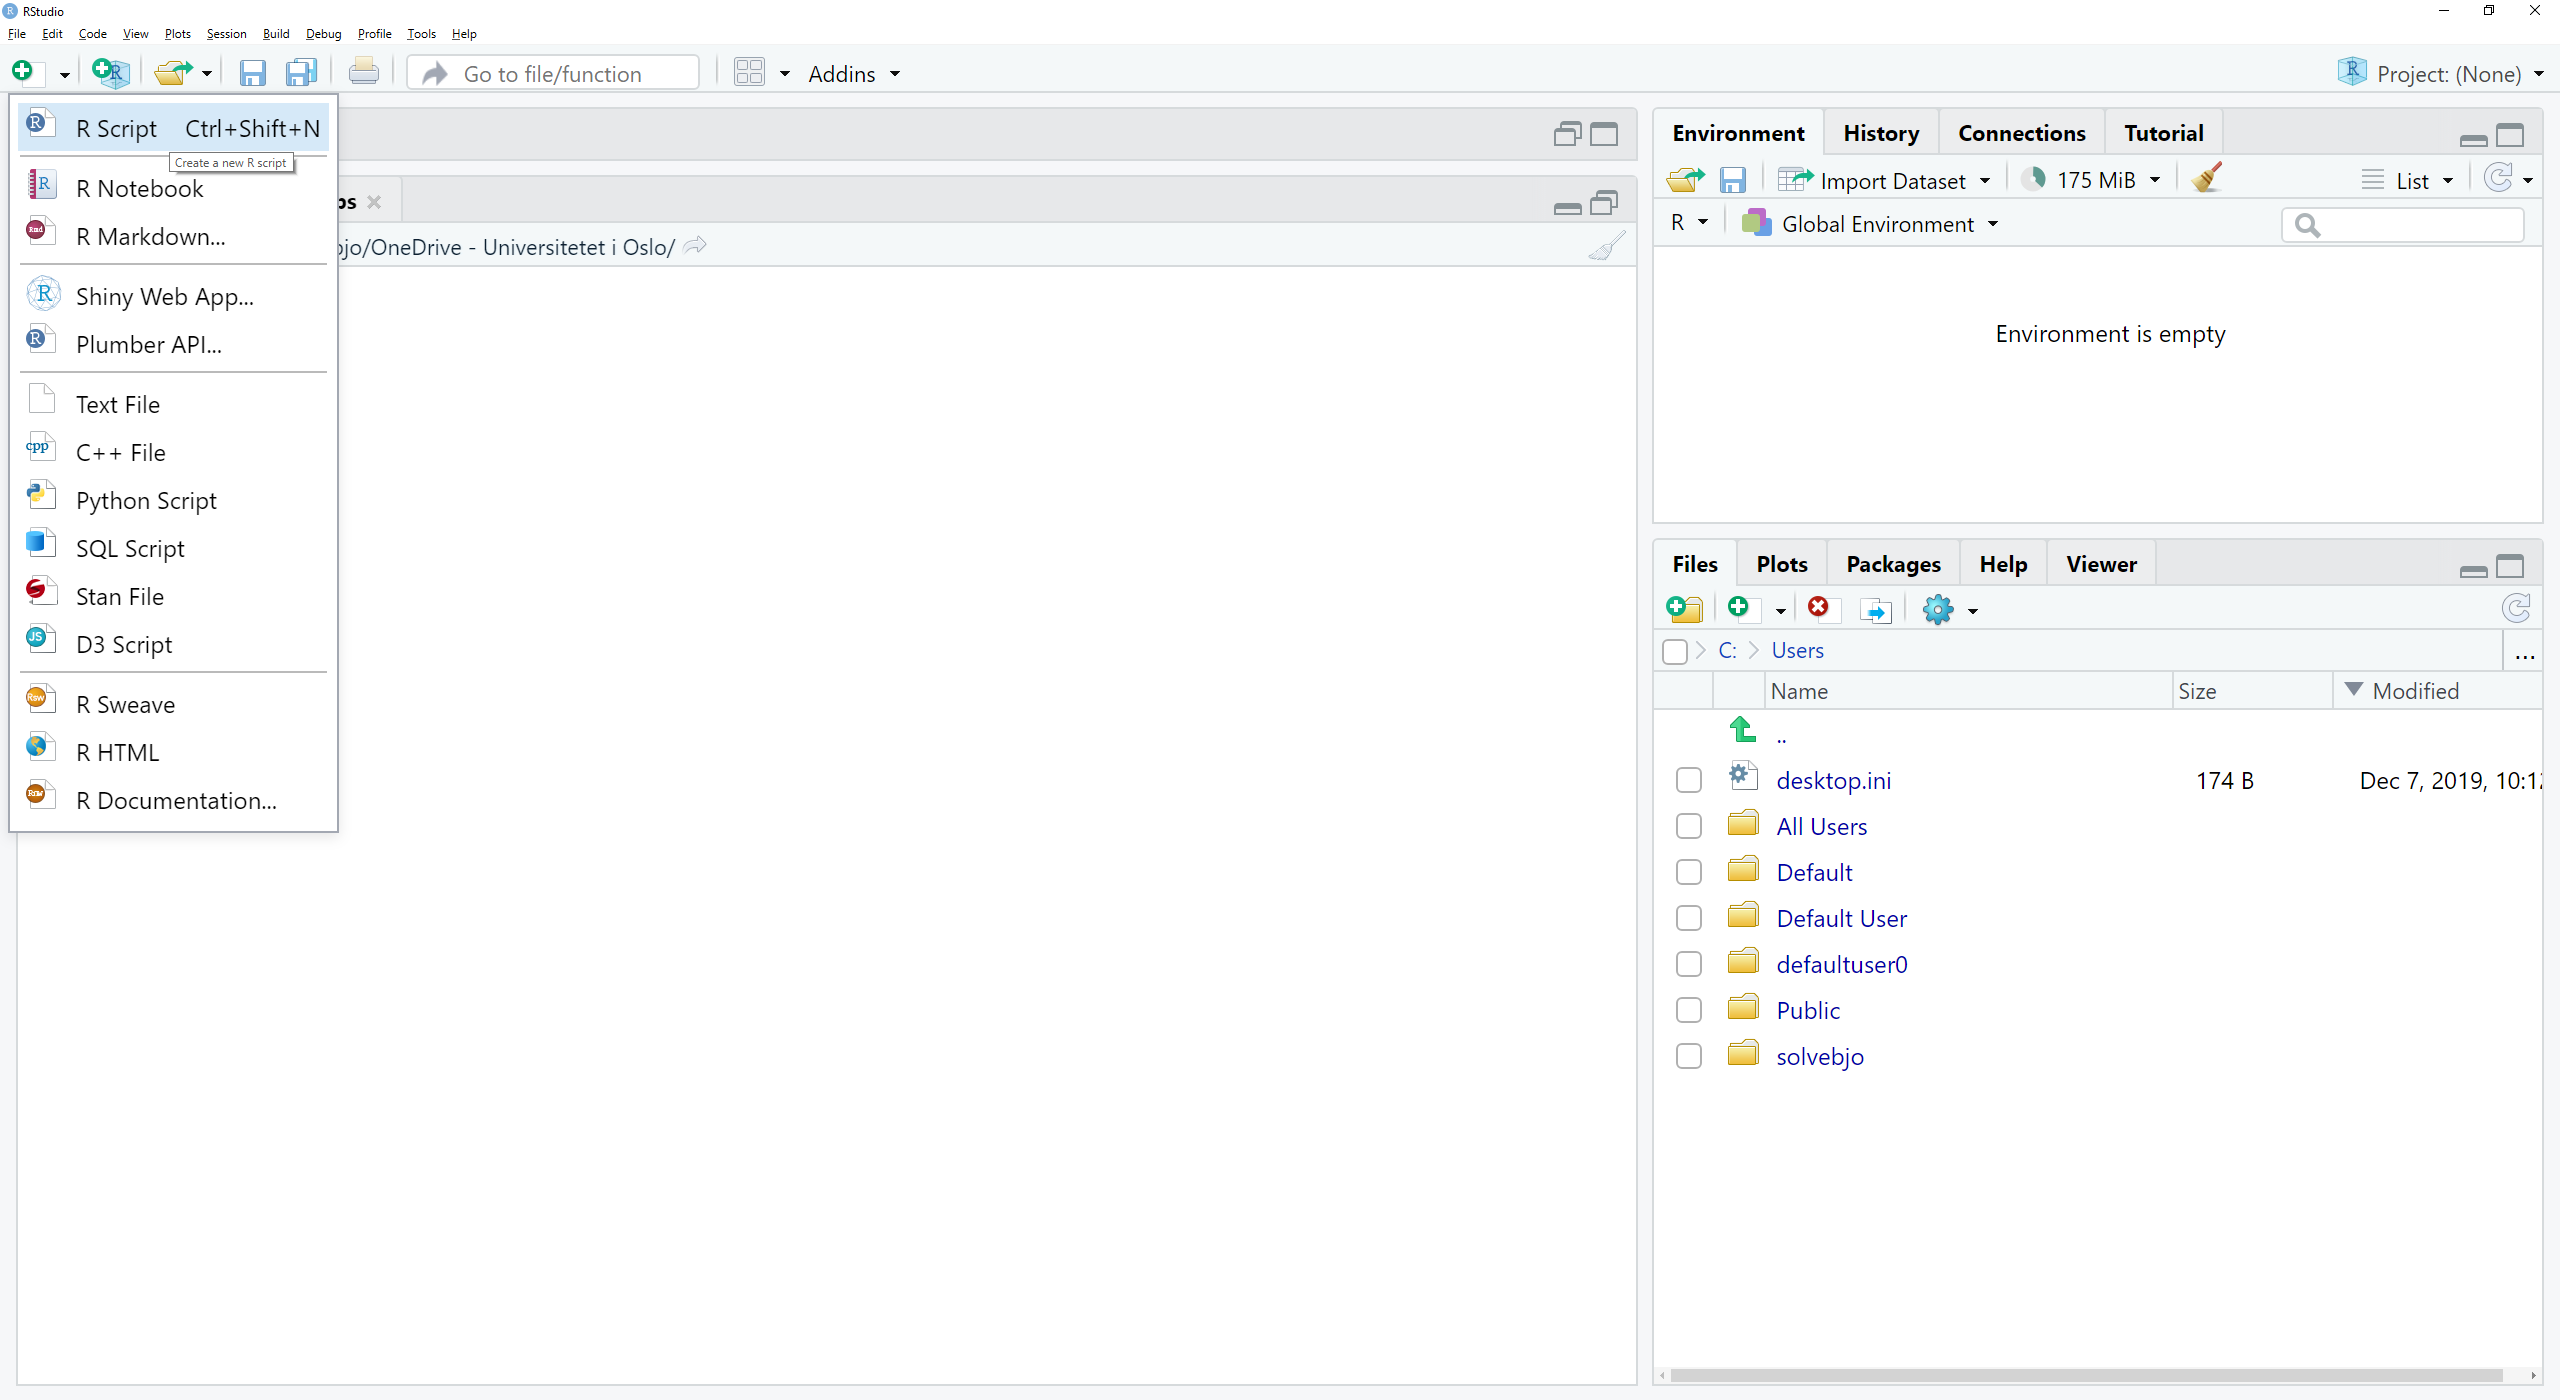
\includegraphics[width=0.8\textwidth,height=\textheight]{./figures/rstudio_2.png}

The script emerges on the top left hand corner of your RStudio
interface. Try typing the following into your script:

\begin{Shaded}
\begin{Highlighting}[]
\DecValTok{1} \SpecialCharTok{+} \DecValTok{1}

\FunctionTok{print}\NormalTok{(}\StringTok{"Hello world!"}\NormalTok{)}

\NormalTok{vector }\OtherTok{\textless{}{-}} \FunctionTok{c}\NormalTok{(}\DecValTok{2}\NormalTok{, }\DecValTok{5}\NormalTok{, }\DecValTok{10}\NormalTok{, }\DecValTok{3}\NormalTok{)}

\FunctionTok{mean}\NormalTok{(vector)}

\FunctionTok{paste}\NormalTok{(}\StringTok{"Hello"}\NormalTok{, }\StringTok{"World"}\NormalTok{, }\StringTok{"!"}\NormalTok{)}

\CommentTok{\# This is a comment.}
\end{Highlighting}
\end{Shaded}

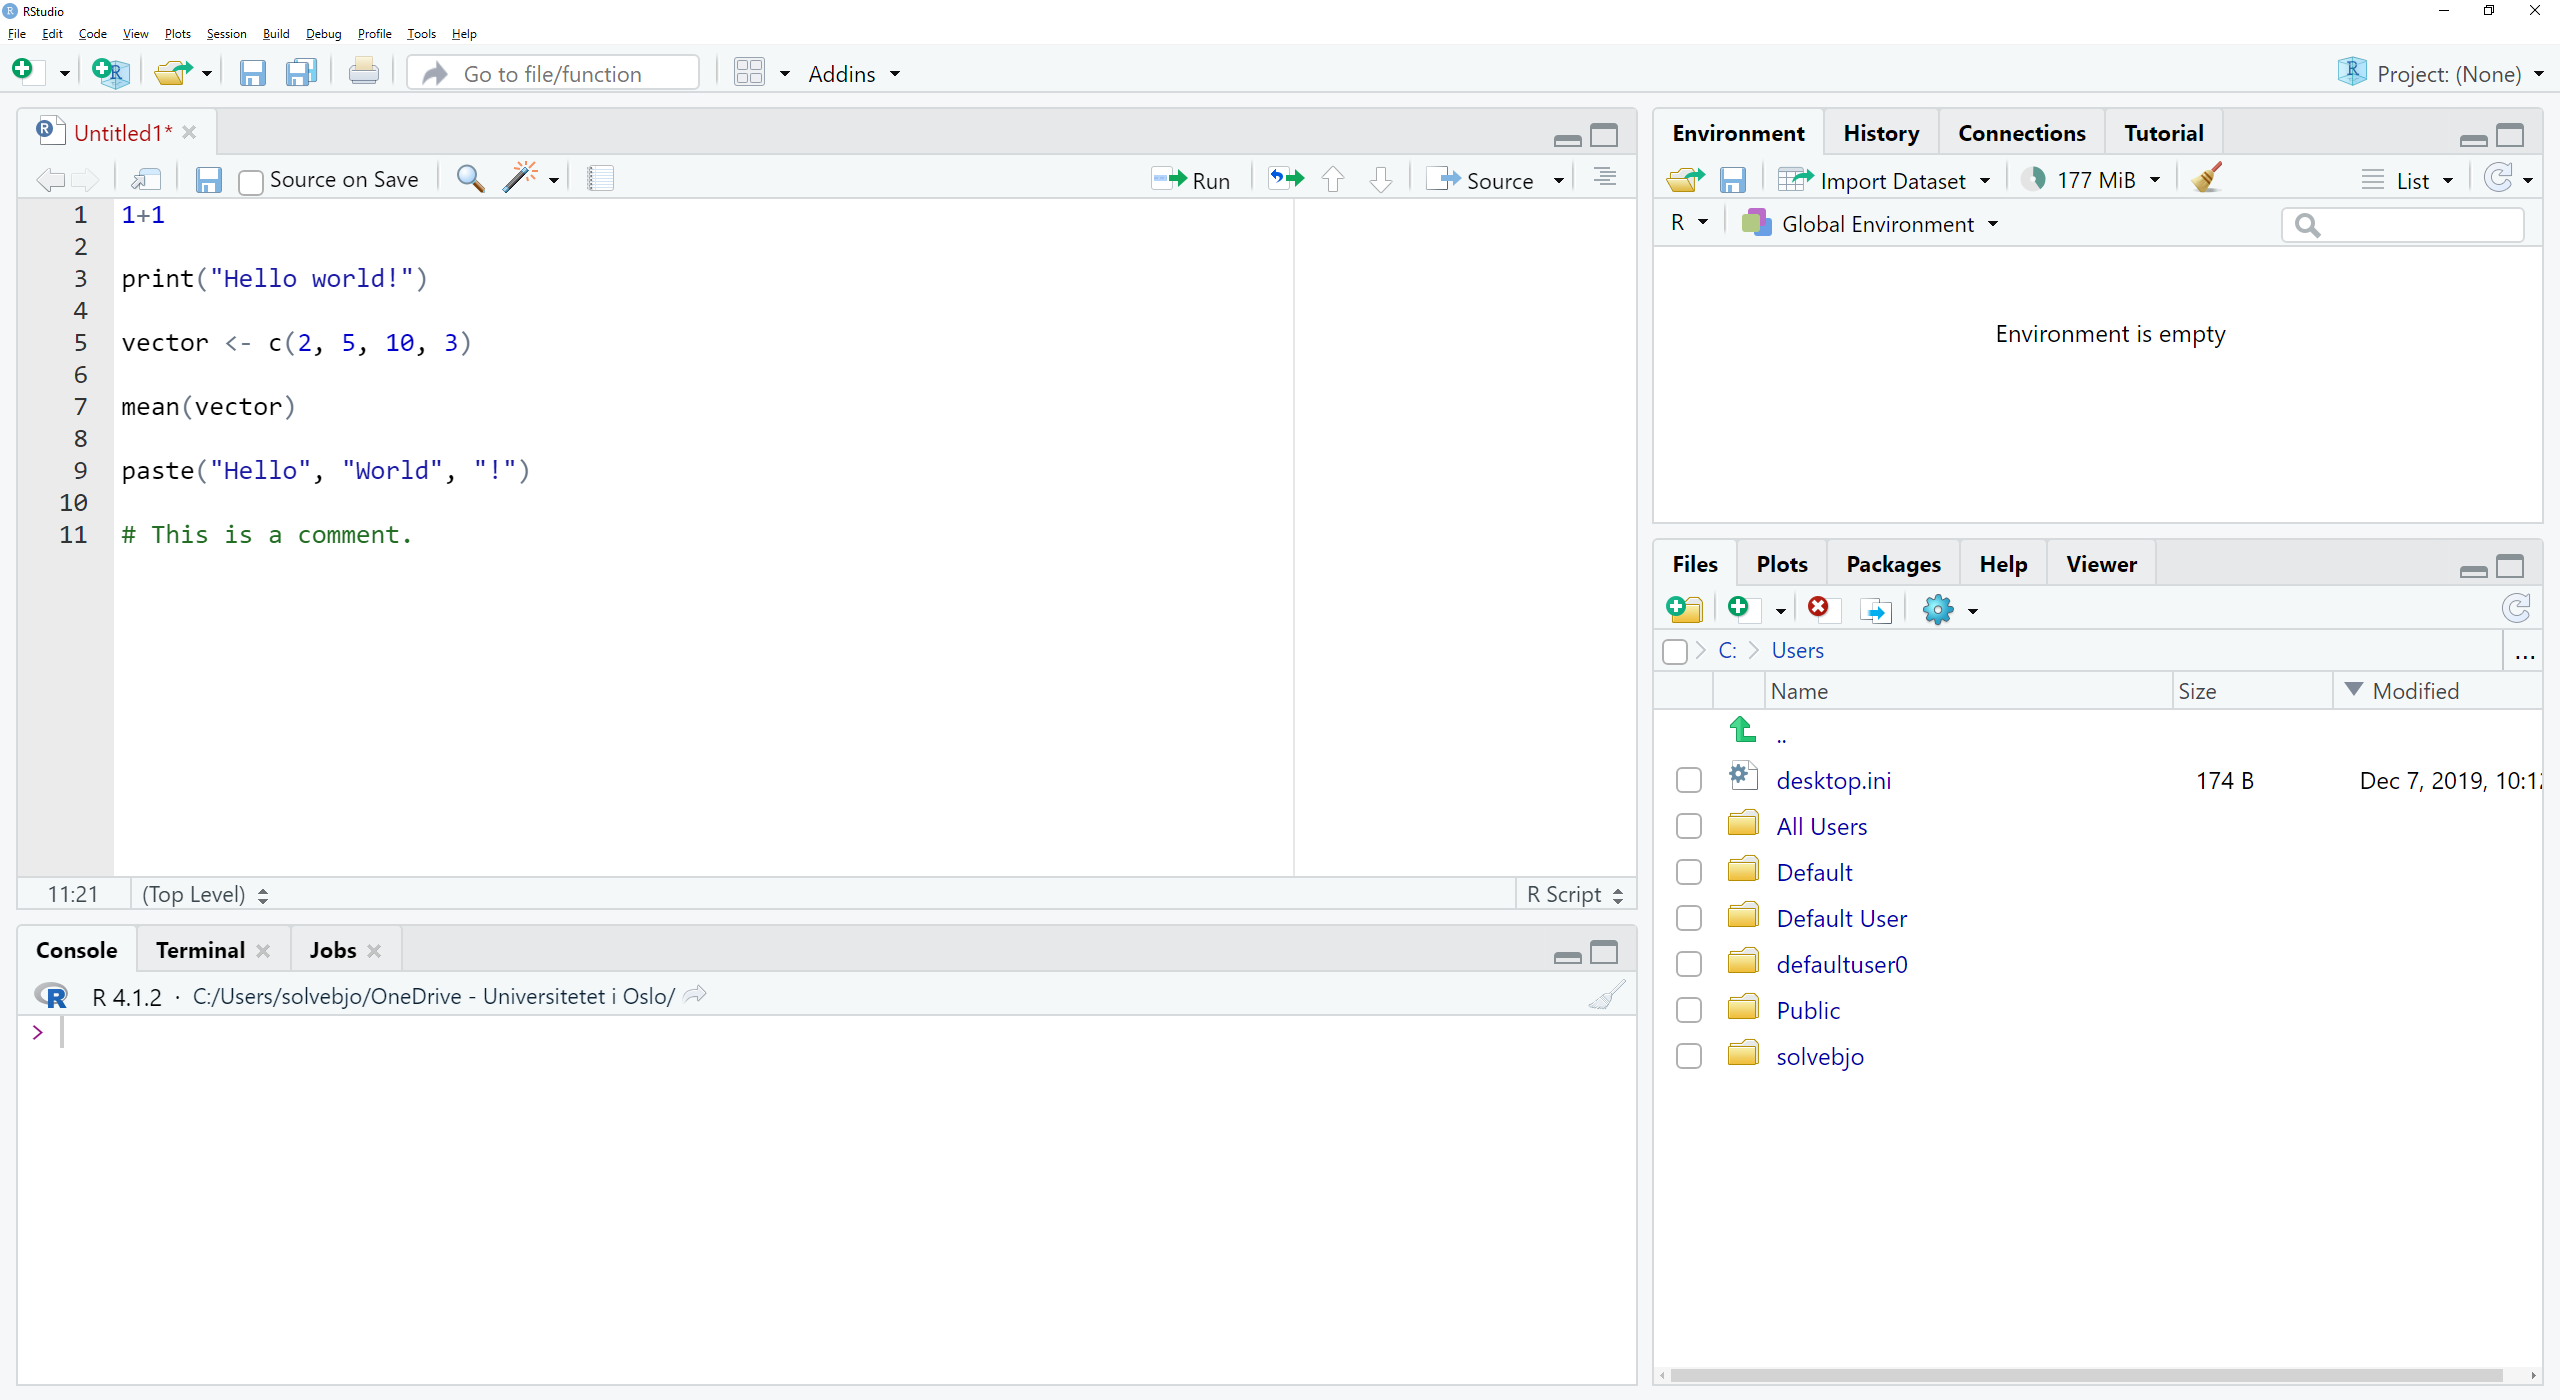
\includegraphics[width=0.8\textwidth,height=\textheight]{./figures/rstudio_3.png}

Then mark the code and click CNTR+ENTER (i.e.~run the code!). The output
from your code appears in the bottom left hand corner of your RStudio
interface. This is called the ``Console''. It's actually where R works,
so you can view it as the engine of the car. All output from your code
will appear here.

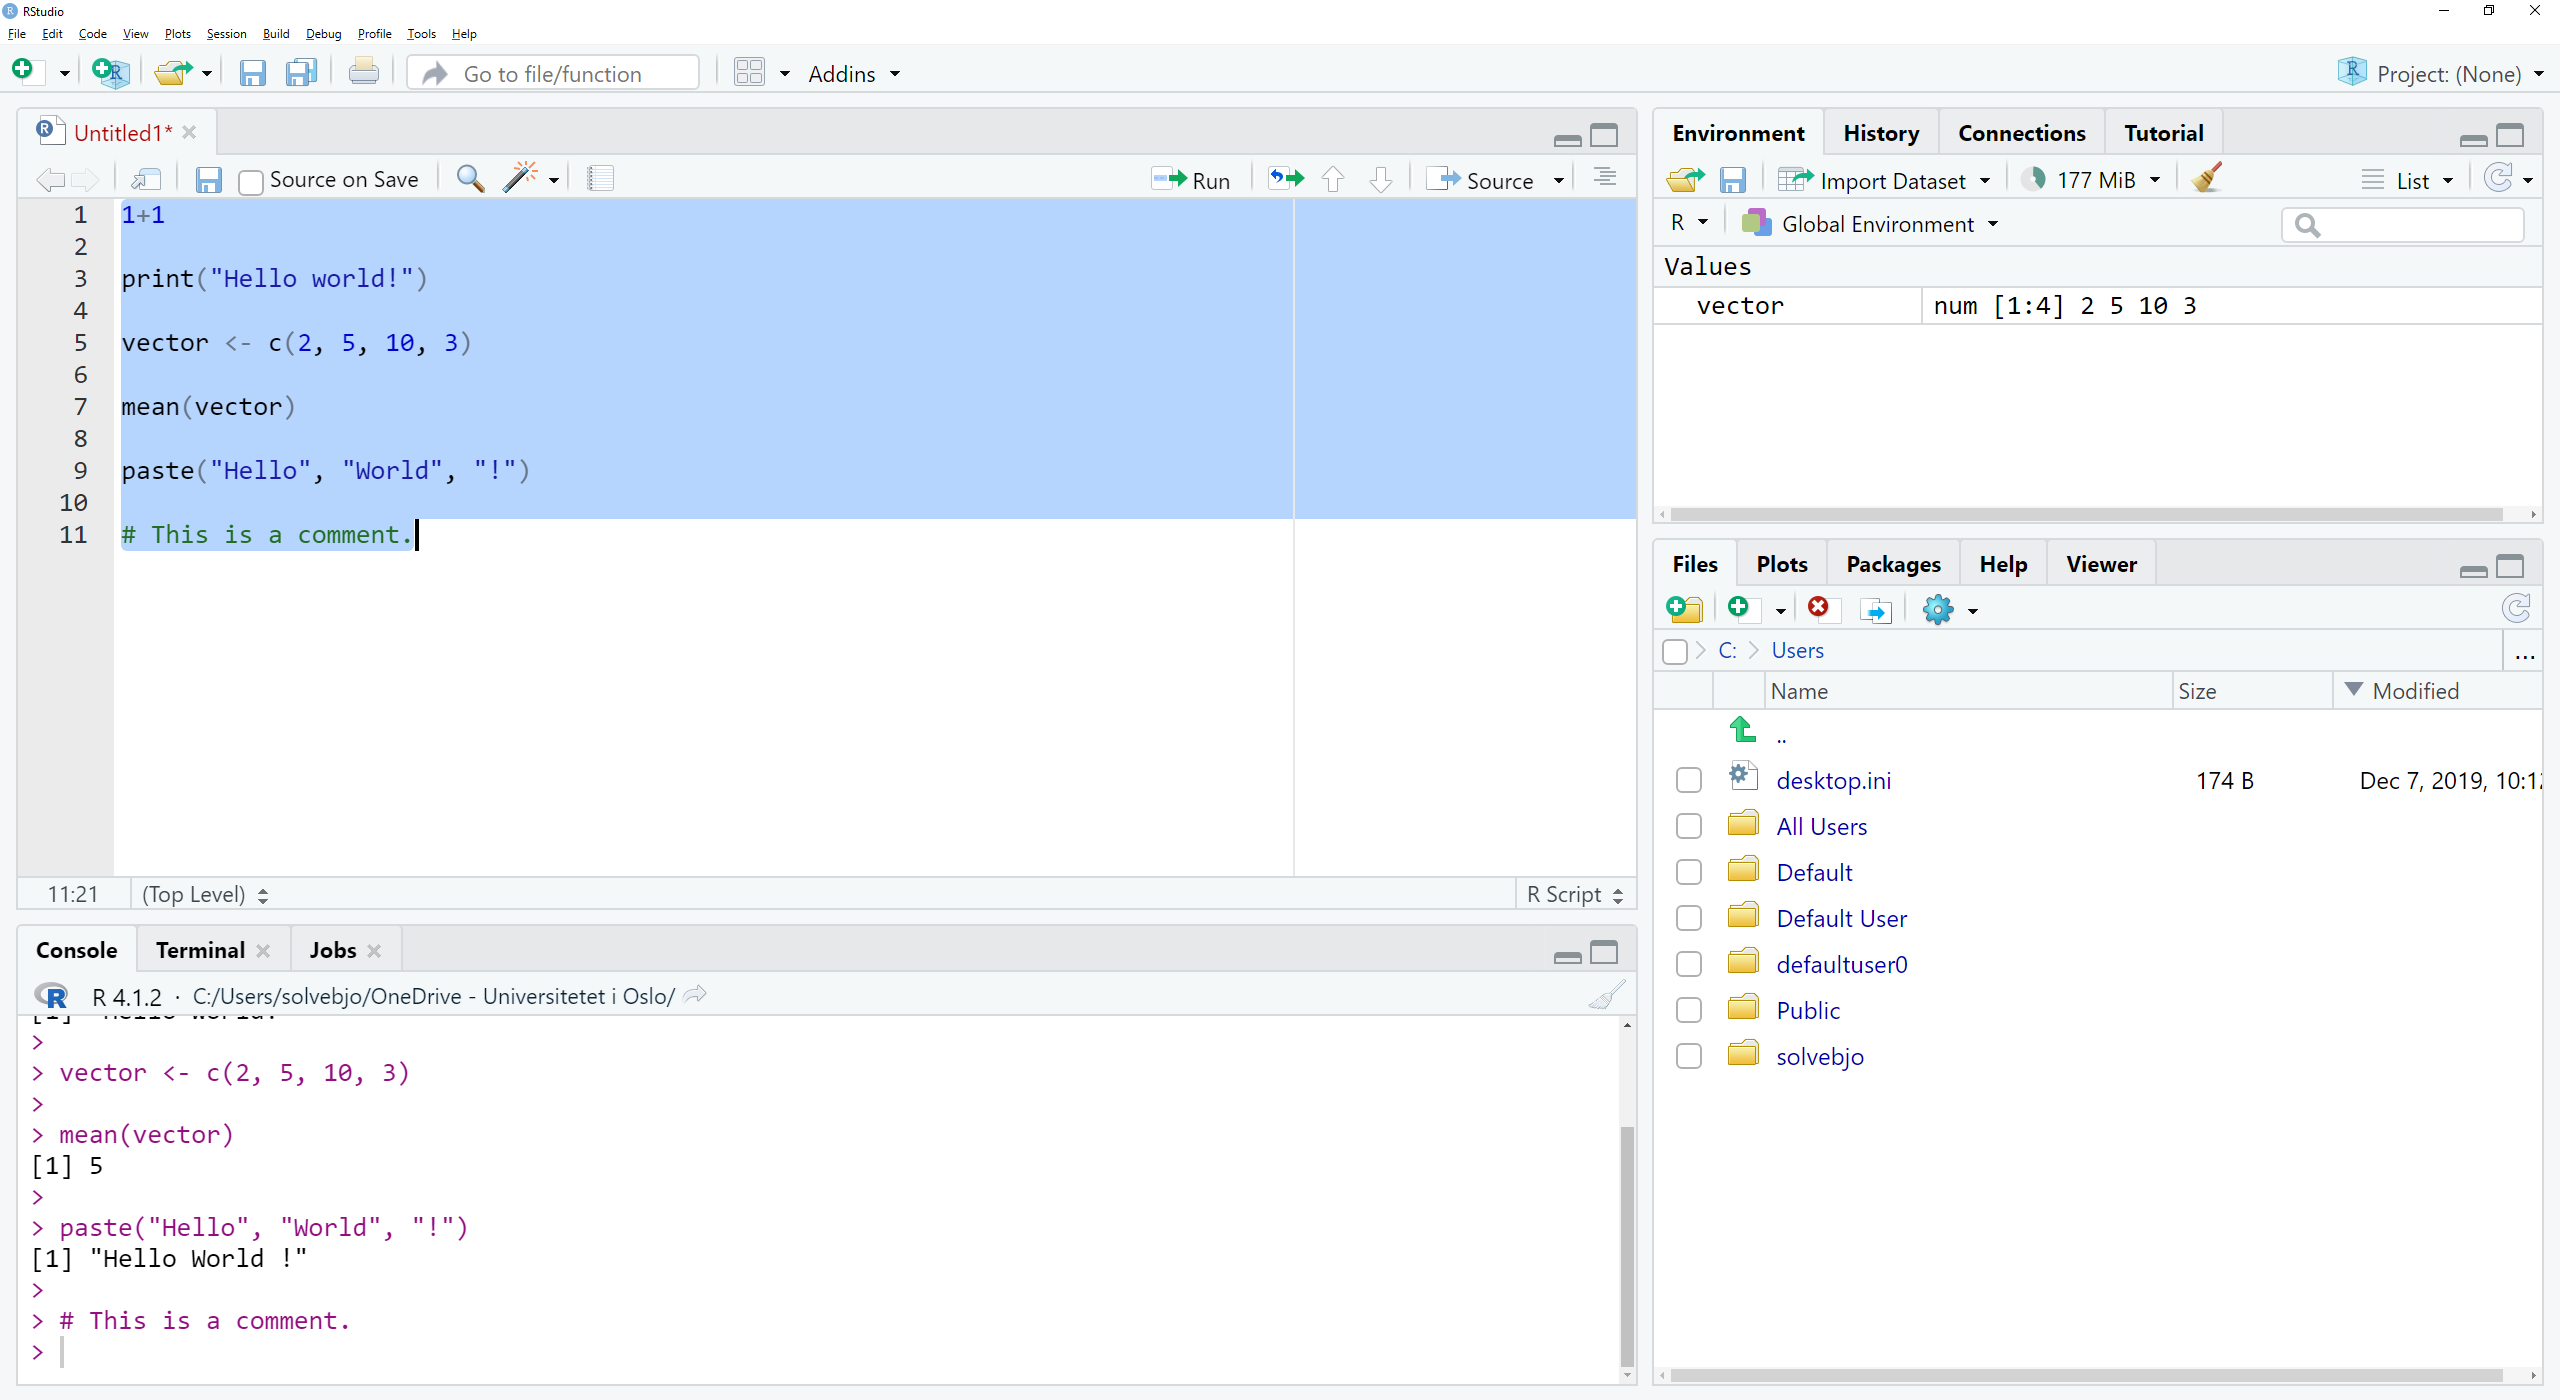
\includegraphics[width=0.8\textwidth,height=\textheight]{./figures/rstudio_4.png}

To save the script, hit the blue disc-symbol as shown in the picture
below.

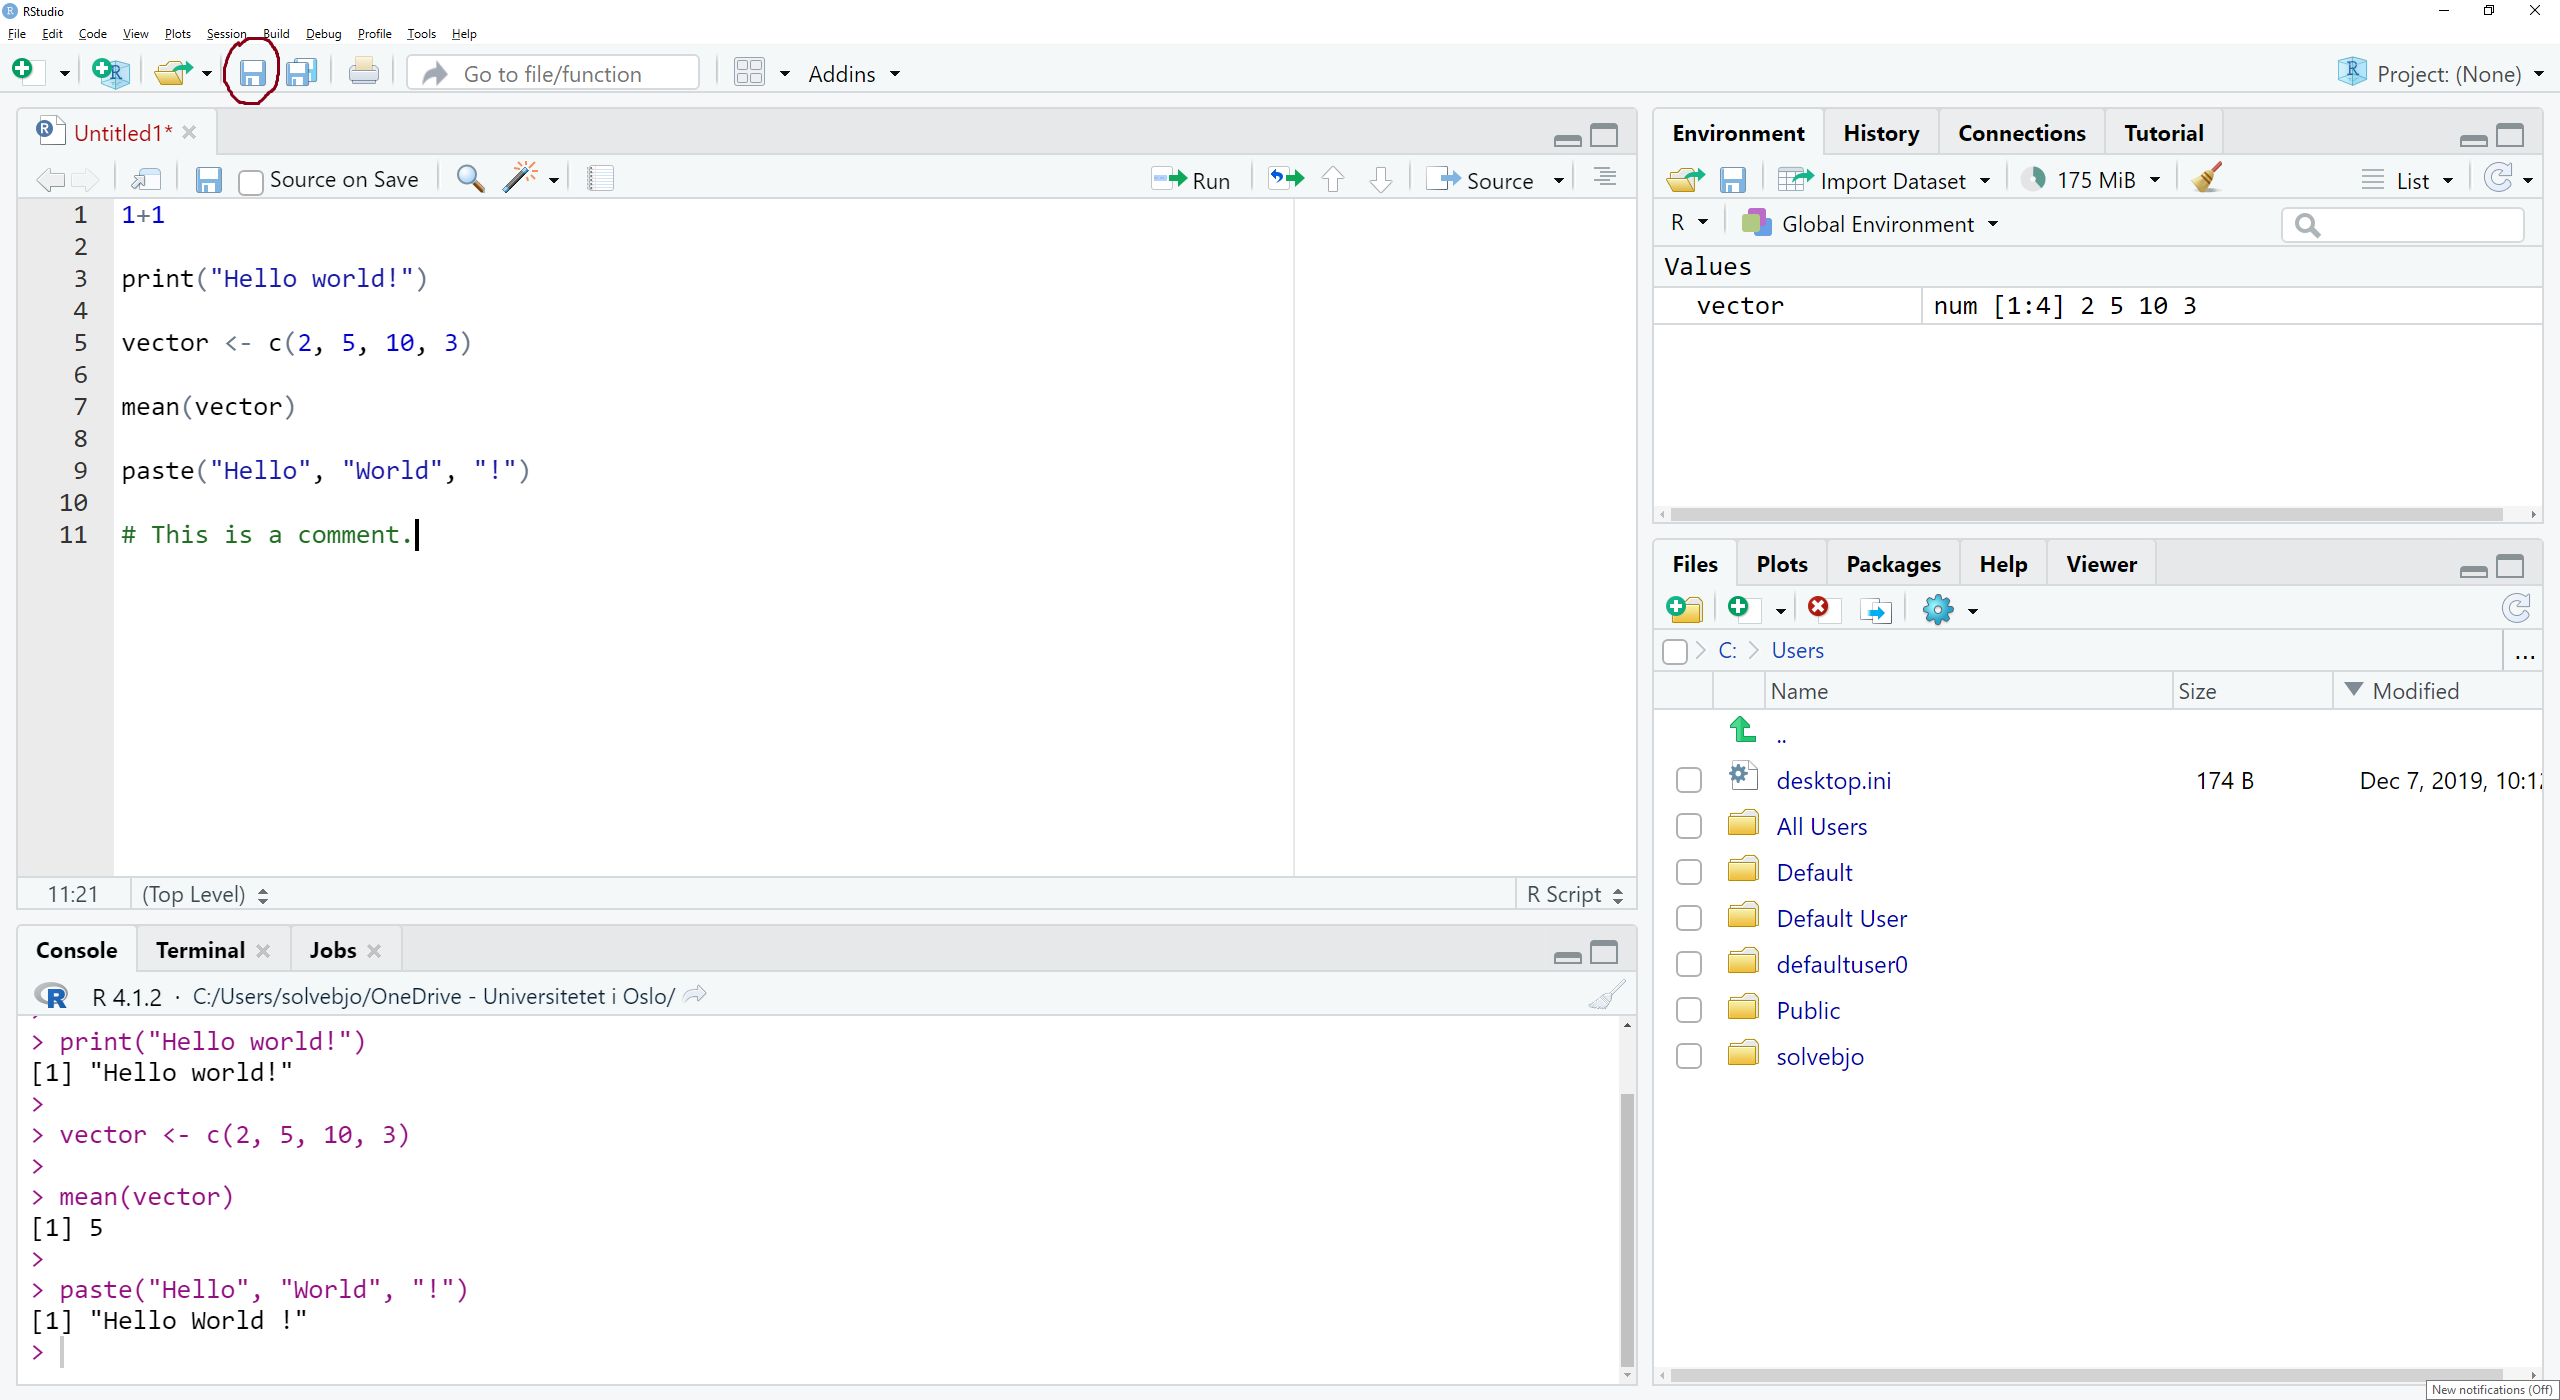
\includegraphics[width=0.8\textwidth,height=\textheight]{./figures/rstudio_5.png}

\hypertarget{objects}{%
\subsection{Objects}\label{objects}}

Notice that something has appeared in the upper right hand corner of
your RStudio interface. This is an object. It has emerged because of
this line in our script:

\begin{Shaded}
\begin{Highlighting}[]
\NormalTok{vector }\OtherTok{\textless{}{-}} \FunctionTok{c}\NormalTok{(}\DecValTok{2}\NormalTok{, }\DecValTok{5}\NormalTok{, }\DecValTok{10}\NormalTok{, }\DecValTok{3}\NormalTok{)}
\end{Highlighting}
\end{Shaded}

This line, because of the arrow (\texttt{\textless{}-}), assigns values
to an object and stores it in the short-term memory of R. The box with
the object is the short-term memory, also known as ``Environment''. We
frequently assign values to objects in R, so it's good to familiarize
yourself with this now. Think: Whenever you want to use an object later,
make an object of it.

In general, to make an object, choose whichever name you like, add an
arrow towards the name of the object, and then add the operation you
want done. If you want to combine several elements, e.g.~several numbers
or several words, you need to put a c in front of your parentheses.
\texttt{c} stands for ``combine''. For example:

\begin{Shaded}
\begin{Highlighting}[]
\NormalTok{numberone }\OtherTok{\textless{}{-}} \DecValTok{1}

\NormalTok{numbers }\OtherTok{\textless{}{-}} \FunctionTok{c}\NormalTok{(}\DecValTok{1}\NormalTok{, }\DecValTok{2}\NormalTok{, }\DecValTok{3}\NormalTok{, }\DecValTok{4}\NormalTok{, }\DecValTok{5}\NormalTok{)}

\NormalTok{meanofnumbers }\OtherTok{\textless{}{-}} \FunctionTok{mean}\NormalTok{(}\FunctionTok{c}\NormalTok{(}\DecValTok{1}\NormalTok{, }\DecValTok{2}\NormalTok{, }\DecValTok{3}\NormalTok{, }\DecValTok{4}\NormalTok{, }\DecValTok{5}\NormalTok{))}

\NormalTok{names }\OtherTok{\textless{}{-}} \FunctionTok{c}\NormalTok{(}\StringTok{"Billy"}\NormalTok{, }\StringTok{"Joe"}\NormalTok{, }\StringTok{"Vera"}\NormalTok{)}
\end{Highlighting}
\end{Shaded}

Why did we call the object ``vector'' in the first place? Because it
\emph{is} a vector. You can think of vectors as a sequence of
information, for example a bunch of numbers or a bunch of names.
\texttt{numberone}, \texttt{meanofnumbers}, \texttt{numbers} and
\texttt{names} are all vectors. There are other types of objects in R.
The ones we will learn are: vector, dataframe, matrix and list. The
difference between them is this:

\begin{itemize}
\tightlist
\item
  Vectors have the same data type and amount to \emph{one} variable.
\item
  Dataframes can have different data types and amount to \emph{several}
  variables.
\item
  Matrices have the same data type and amount to \emph{several}
  variables.
\item
  Lists have several types of data types and amount to \emph{one} or
  \emph{several} variables.\footnote{Some illustrations of data objects
    in R also operate with arrays, but we will not focus on that here.}
\end{itemize}

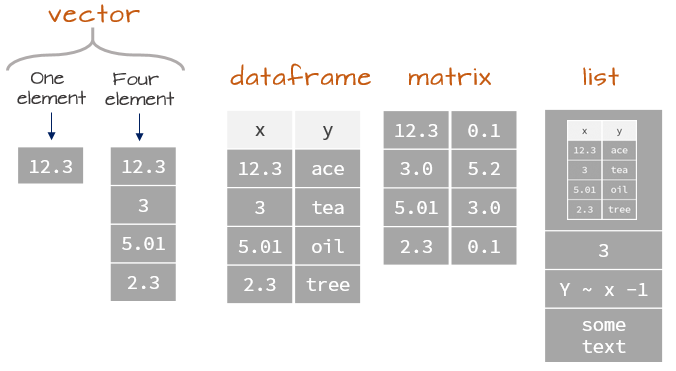
\includegraphics[width=0.8\textwidth,height=\textheight]{./figures/objects.png}

To know what an object contains, try writing the name of the object and
run it\footnote{To ``run a code'' means to mark it and hit CNTR+ENTER}.

\hypertarget{data-types}{%
\subsection{Data types}\label{data-types}}

What does ``data type'' mean, then? Well, R has several data types and
we will focus on four\footnote{Some people also add ``complex'' as a
  data type, but this is outside our scope.}. These are
\texttt{numeric}, \texttt{integer}, \texttt{character}, \texttt{factor}
and \texttt{logical}, and they are also called \emph{classes}. They
differ from each other in the types of data they store, be it strings,
numbers or logical values.

\begin{longtable}[]{@{}
  >{\raggedright\arraybackslash}p{(\columnwidth - 2\tabcolsep) * \real{0.1831}}
  >{\centering\arraybackslash}p{(\columnwidth - 2\tabcolsep) * \real{0.8169}}@{}}
\toprule
\begin{minipage}[b]{\linewidth}\raggedright
Data type
\end{minipage} & \begin{minipage}[b]{\linewidth}\centering
Properties
\end{minipage} \\
\midrule
\endhead
\texttt{numeric} & contains decimal and whole numbers, also called
``double'' \\
\texttt{integer} & contains only whole numbers \\
\texttt{character} & contains character strings (``words'') \\
\texttt{factor} & contains categories (either ranked or unranked) \\
\texttt{logical} & contains only two values, TRUE and FALSE \\
\bottomrule
\end{longtable}

Numbers and integers can be one number, sequences of numbers, or
mathematical expressions. For example:

\begin{Shaded}
\begin{Highlighting}[]
\DecValTok{100}

\DecValTok{1} \SpecialCharTok{+} \DecValTok{100} \SpecialCharTok{+} \DecValTok{20}

\FloatTok{1.4353}  \CommentTok{\# commas are written as dots (.)}

\FloatTok{1.5} \SpecialCharTok{+} \FloatTok{2.9} \SpecialCharTok{{-}} \FloatTok{8.3}

\DecValTok{2} \SpecialCharTok{*} \DecValTok{8}  \CommentTok{\# multiply is written as star (*)}

\DecValTok{9}\SpecialCharTok{/}\DecValTok{3}  \CommentTok{\# divide is written as slash (/)}

\FunctionTok{c}\NormalTok{(}\DecValTok{3}\NormalTok{, }\DecValTok{100}\NormalTok{, }\FloatTok{203.4}\NormalTok{, }\DecValTok{15000}\NormalTok{)}
\end{Highlighting}
\end{Shaded}

Strings are sequences of characters, often words. We need to surround
them in quotation marks. For example:

\begin{Shaded}
\begin{Highlighting}[]
\StringTok{"A"}

\FunctionTok{c}\NormalTok{(}\StringTok{"A"}\NormalTok{, }\StringTok{"B"}\NormalTok{)  }\CommentTok{\# If \textquotesingle{}A\textquotesingle{} and \textquotesingle{}B\textquotesingle{} were two categories, this object could also be a factor.}

\StringTok{"Hello"}

\StringTok{"We are learning R!"}

\FunctionTok{c}\NormalTok{(}\StringTok{"Hello."}\NormalTok{, }\StringTok{"We are learning R!"}\NormalTok{)}
\end{Highlighting}
\end{Shaded}

Logical vectors take two values; TRUE and FALSE.

\begin{Shaded}
\begin{Highlighting}[]
\ConstantTok{TRUE}

\ConstantTok{FALSE}

\FunctionTok{c}\NormalTok{(}\ConstantTok{TRUE}\NormalTok{, }\ConstantTok{FALSE}\NormalTok{, }\ConstantTok{FALSE}\NormalTok{, }\ConstantTok{FALSE}\NormalTok{, }\ConstantTok{TRUE}\NormalTok{)}
\end{Highlighting}
\end{Shaded}

To check the data type, use the function \texttt{class()}.

\begin{Shaded}
\begin{Highlighting}[]
\FunctionTok{class}\NormalTok{(}\DecValTok{100}\NormalTok{)}
\end{Highlighting}
\end{Shaded}

\begin{verbatim}
## [1] "numeric"
\end{verbatim}

\begin{Shaded}
\begin{Highlighting}[]
\FunctionTok{class}\NormalTok{(}\StringTok{"A"}\NormalTok{)}
\end{Highlighting}
\end{Shaded}

\begin{verbatim}
## [1] "character"
\end{verbatim}

\begin{Shaded}
\begin{Highlighting}[]
\FunctionTok{class}\NormalTok{(}\ConstantTok{FALSE}\NormalTok{)}
\end{Highlighting}
\end{Shaded}

\begin{verbatim}
## [1] "logical"
\end{verbatim}

\hypertarget{logical-operators}{%
\subsection{Logical operators}\label{logical-operators}}

At last, we can use different operators to check whether to objects are
equal to each other. We wil not delve into this now, but I leave this
here because it might be useful later.

\begin{longtable}[]{@{}lc@{}}
\toprule
Operator & Meaning \\
\midrule
\endhead
\texttt{==} & equals \\
\texttt{\textless{}} & less than \\
\texttt{\textgreater{}} & bigger than \\
\texttt{\textless{}=} & less than or equals \\
\texttt{\textgreater{}=} & bigger than or equals \\
\texttt{!=} & does not equal \\
\texttt{!x} & does not equal x \\
\texttt{\textbar{}} & or \\
\texttt{\&} & and \\
\bottomrule
\end{longtable}

\hypertarget{calling-functions}{%
\section{Calling functions}\label{calling-functions}}

As you can see, we can use R as a calculator if we want to. Writing
\texttt{1+1} gives \texttt{2} in the Console. But the real power of R
comes from running functions. A function is a command that tells R what
to do with something. We've already seen a few functions so far, for
example \texttt{print()}, \texttt{mean()} and \texttt{class()}.
\texttt{print()} tells R to give us the output of an object,
\texttt{mean()} tells R to calculate the average of an object, and
\texttt{class()} tells R to give us the data type of an object.

Learning functions is a bit like learning vocabulary in a language, so
don't fret if you find yourself grasping for the name of a function.
It's the same as when you somewhat know a language and can't really
recall a word. The solution? Ask someone or look it up on the internet.

\hypertarget{packages}{%
\subsection{Packages}\label{packages}}

Most functions we get from packages. Packages are bundles of functions
that we import to R, and they are made by the wide community of people
out there who work on R-content. For example, \texttt{stringr} is a
package that gives us a lot of functions we can use to work with strings
(i.e.~character things). Some of these functions are
\texttt{str\_to\_lower()}, which make all characters into lower case,
\texttt{str\_repalce}, which takes part of a string and replaces it with
something else, and \texttt{sub\_str()}, which takes out a part of a
string.

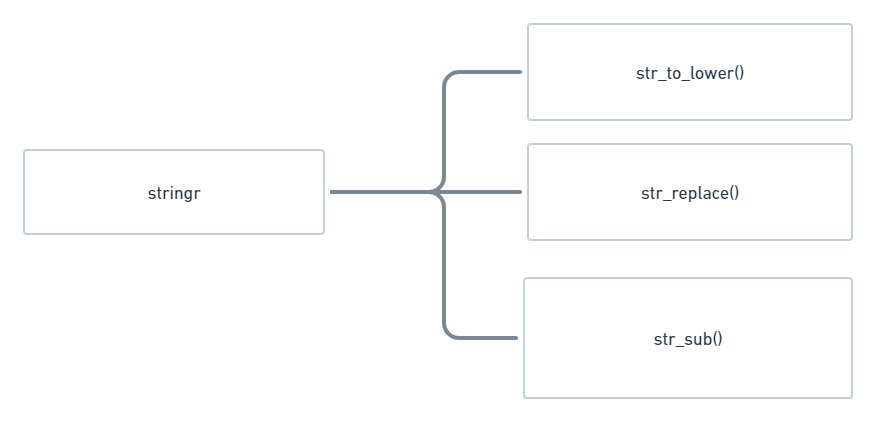
\includegraphics[width=0.8\textwidth,height=\textheight]{./figures/packages.png}

To get a package into R, we first have to install it (from the world
wide web), then import it (telling R that we want to use it in this
script).

To install a package, use the function \texttt{install.packages()} and
put the name of the package in quotation marks. You only need to do this
\emph{once} (unless you uninstall and reinstall R, or want to update
your packages to newer versions). So no need to populate your script
with \texttt{install.packages()}.

\begin{Shaded}
\begin{Highlighting}[]
\FunctionTok{install.packages}\NormalTok{(}\StringTok{"string"}\NormalTok{)}
\end{Highlighting}
\end{Shaded}

To import a package, use the function \texttt{library()}. Here, you do
not need quotation marks.

\begin{Shaded}
\begin{Highlighting}[]
\FunctionTok{library}\NormalTok{(stringr)}
\end{Highlighting}
\end{Shaded}

\begin{verbatim}
## Warning: package 'stringr' was built under R version 4.1.3
\end{verbatim}

Once this is in order, we can start using functions from the package
\texttt{stringr}. A full overview of all the functions in a package is
available on the internet through a document that all package-makers
have to make for their package. In the case of \texttt{stringr}, a quick
internet search leads us to
\href{https://cran.r-project.org/web/packages/stringr/stringr.pdf}{this
document}.

Let's try some of the functions!

\begin{Shaded}
\begin{Highlighting}[]
\NormalTok{string }\OtherTok{\textless{}{-}} \StringTok{"This is a string, meaning a sequence of characters, typically words. It is also a vector, since it contains information of one data type {-} namely character."}

\FunctionTok{print}\NormalTok{(string)}
\end{Highlighting}
\end{Shaded}

\begin{verbatim}
## [1] "This is a string, meaning a sequence of characters, typically words. It is also a vector, since it contains information of one data type - namely character."
\end{verbatim}

\begin{Shaded}
\begin{Highlighting}[]
\FunctionTok{str\_to\_lower}\NormalTok{(string)  }\CommentTok{\# Sets all characters to lower case.}
\end{Highlighting}
\end{Shaded}

\begin{verbatim}
## [1] "this is a string, meaning a sequence of characters, typically words. it is also a vector, since it contains information of one data type - namely character."
\end{verbatim}

\begin{Shaded}
\begin{Highlighting}[]
\FunctionTok{str\_replace}\NormalTok{(string, }\StringTok{"This is a string, meaning a"}\NormalTok{, }\StringTok{"A string is a"}\NormalTok{)  }\CommentTok{\# Replaces some parts of a string with something else.}
\end{Highlighting}
\end{Shaded}

\begin{verbatim}
## [1] "A string is a sequence of characters, typically words. It is also a vector, since it contains information of one data type - namely character."
\end{verbatim}

\begin{Shaded}
\begin{Highlighting}[]
\FunctionTok{str\_sub}\NormalTok{(string, }\DecValTok{1}\NormalTok{, }\DecValTok{16}\NormalTok{)  }\CommentTok{\# Picks out characters from place 1 to place 16.}
\end{Highlighting}
\end{Shaded}

\begin{verbatim}
## [1] "This is a string"
\end{verbatim}

\hypertarget{your-own-functions}{%
\subsection{Your own functions}\label{your-own-functions}}

You can make your own functions too.

\begin{Shaded}
\begin{Highlighting}[]
\NormalTok{make\_lower\_and\_pick\_start }\OtherTok{\textless{}{-}} \ControlFlowTok{function}\NormalTok{(x) \{}

\NormalTok{    x }\OtherTok{\textless{}{-}} \FunctionTok{str\_to\_lower}\NormalTok{(x)}
\NormalTok{    x }\OtherTok{\textless{}{-}} \FunctionTok{str\_sub}\NormalTok{(x, }\DecValTok{1}\NormalTok{, }\DecValTok{16}\NormalTok{)}

    \FunctionTok{return}\NormalTok{(x)}

\NormalTok{\}}

\FunctionTok{make\_lower\_and\_pick\_start}\NormalTok{(string)}
\end{Highlighting}
\end{Shaded}

\begin{verbatim}
## [1] "this is a string"
\end{verbatim}

\hypertarget{installing-latex}{%
\subsubsection{Installing LaTex}\label{installing-latex}}

Now that we know how to work with packages, let's tackle the fact that
we're going to write in RMarkdown. The great thing about R Markdown is
that we can produce nice reports, for example in PDF. However, we need
LaTex to make R Markdown reports in PDF, so we need to install this as
well.

LaTex is a document preparation system, much like word, except it is
more code-heavy and allows you to create beautiful documents. TinyTex is
a custom LaTeX distribution, so this is what we'll install. See
\url{https://yihui.org/tinytex/} for more informaton.

To install TinyTex from R, we need to install the package
\texttt{tinytex} and use the function \texttt{install\_tinytex()}.

\begin{Shaded}
\begin{Highlighting}[]
\FunctionTok{install.packages}\NormalTok{(}\StringTok{"tinytex"}\NormalTok{)}
\FunctionTok{install\_tinytex}\NormalTok{()}
\CommentTok{\# to uninstall TinyTeX, run tinytex::uninstall\_tinytex()}
\end{Highlighting}
\end{Shaded}

\hypertarget{introduction-to-r-markdown-and-jupyter-notebooks}{%
\section{Introduction to R Markdown (and Jupyter
Notebooks)}\label{introduction-to-r-markdown-and-jupyter-notebooks}}

R Markdown is a type of script that contains both text and code, and
that can be turned into both documents and web pages. It's very handy in
that regard. To open an R Markdown file in RStudio, click ``File'',
``New file'' and ``R Markdown''. Or, alternatively, click the document
sign on the top left corner of your RStudio interface and choose ``R
Markdown''. You'll get a box asking you for the title of your document.
Call it whatever you like, then hit OK.

For those curious: R Markdown is a way to integrate writing in Markdown
through R. Markdown is a markup language which, guess what, is also a
type of computer language! In other words, we use it to speak with the
computer, telling the computer the different properties of our text, be
it a title, \textbf{bold}, \emph{italics} or \texttt{code}. However, in
contrast to for example R, python and Java, markup languages are much
easier to read by humans. Other examples of markup languages are HTML
and XML. This is not super important to know in order to write in R
Markdown, but it's nice with a bit of context now and then.

Now, your RStudio interface should look something like the picture
below. Notice the ``Knit'' button at the top, and try clicking it. It
will prompt a request to save your file on your computer, and once
you've done that, the R Markdown will convert your code into a nice HTML
report\footnote{HTML is the language of the web. Most webpages are
  written in HTML.} Navigate to where you saved your file, click on the
name of the file with the ``.html'' ending, and open it in an internet
browser (such as Firefox or Chrome).

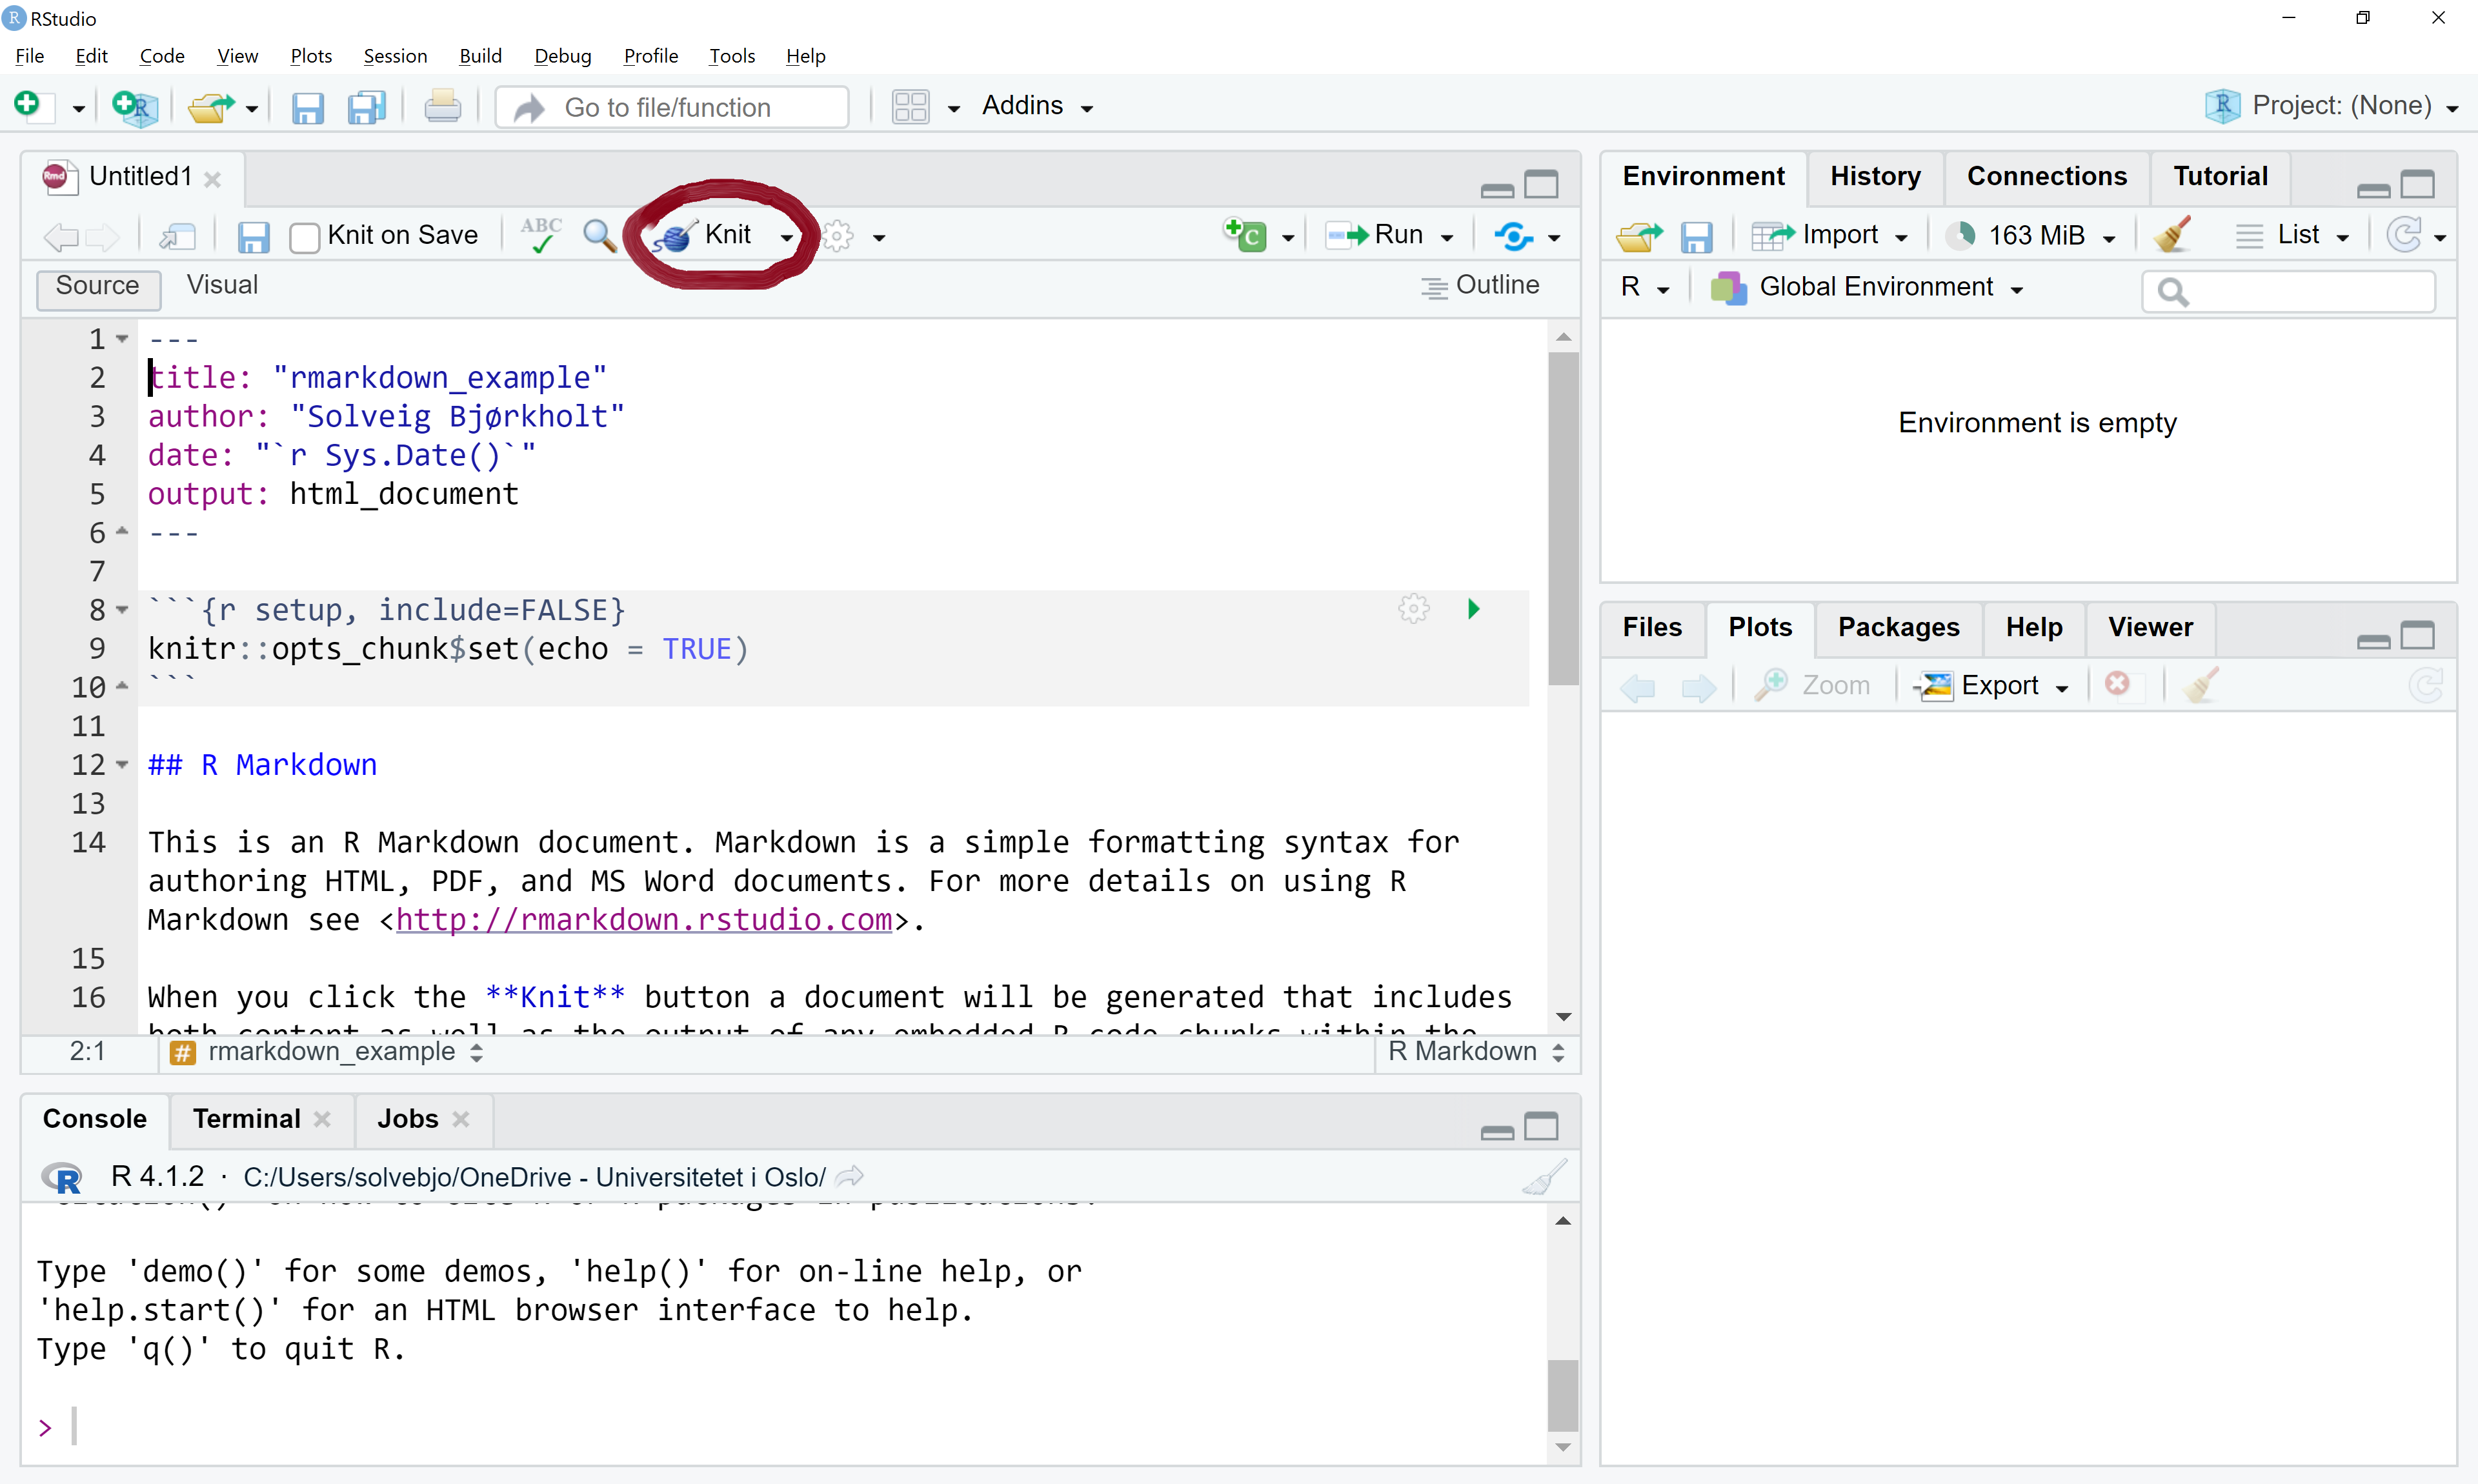
\includegraphics[width=0.8\textwidth,height=\textheight]{./figures/rmarkdown_2.png}

To modify the report, here are a few things to know:

\begin{itemize}
\tightlist
\item
  In the beginning of the document, the
  \texttt{knitr::opts\_chuck\$set(echo\ =\ FALSE)} tells R to use the
  \texttt{opts\_chuck} function from the \texttt{knitr} package, and to
  modify the object set. In here, you can modify what you want the
  general settings of the document to be. \texttt{echo\ =\ FALSE} means
  that you do not want code to show typically, just the output of it.
  Other options are for example \texttt{include} (whether to typically
  include chunks) and \texttt{warnings} (whether to typically show
  warning messages from code).
\end{itemize}

To add a chuck of code, add the hyphens, curly parentheses and the r,
and end with three curly parentheses as well. In the middle, write your
code.

\texttt{\textasciigrave{}\textasciigrave{}\textasciigrave{}\{r\}}

\texttt{\textasciigrave{}\textasciigrave{}\textasciigrave{}}

For more settings, consult the image below, also available
\href{https://www.rstudio.com/wp-content/uploads/2015/02/rmarkdown-cheatsheet.pdf}{here},
and search around on the internet whenever you wonder about something.
The best way to learn is to just start and look up things as you need
them.

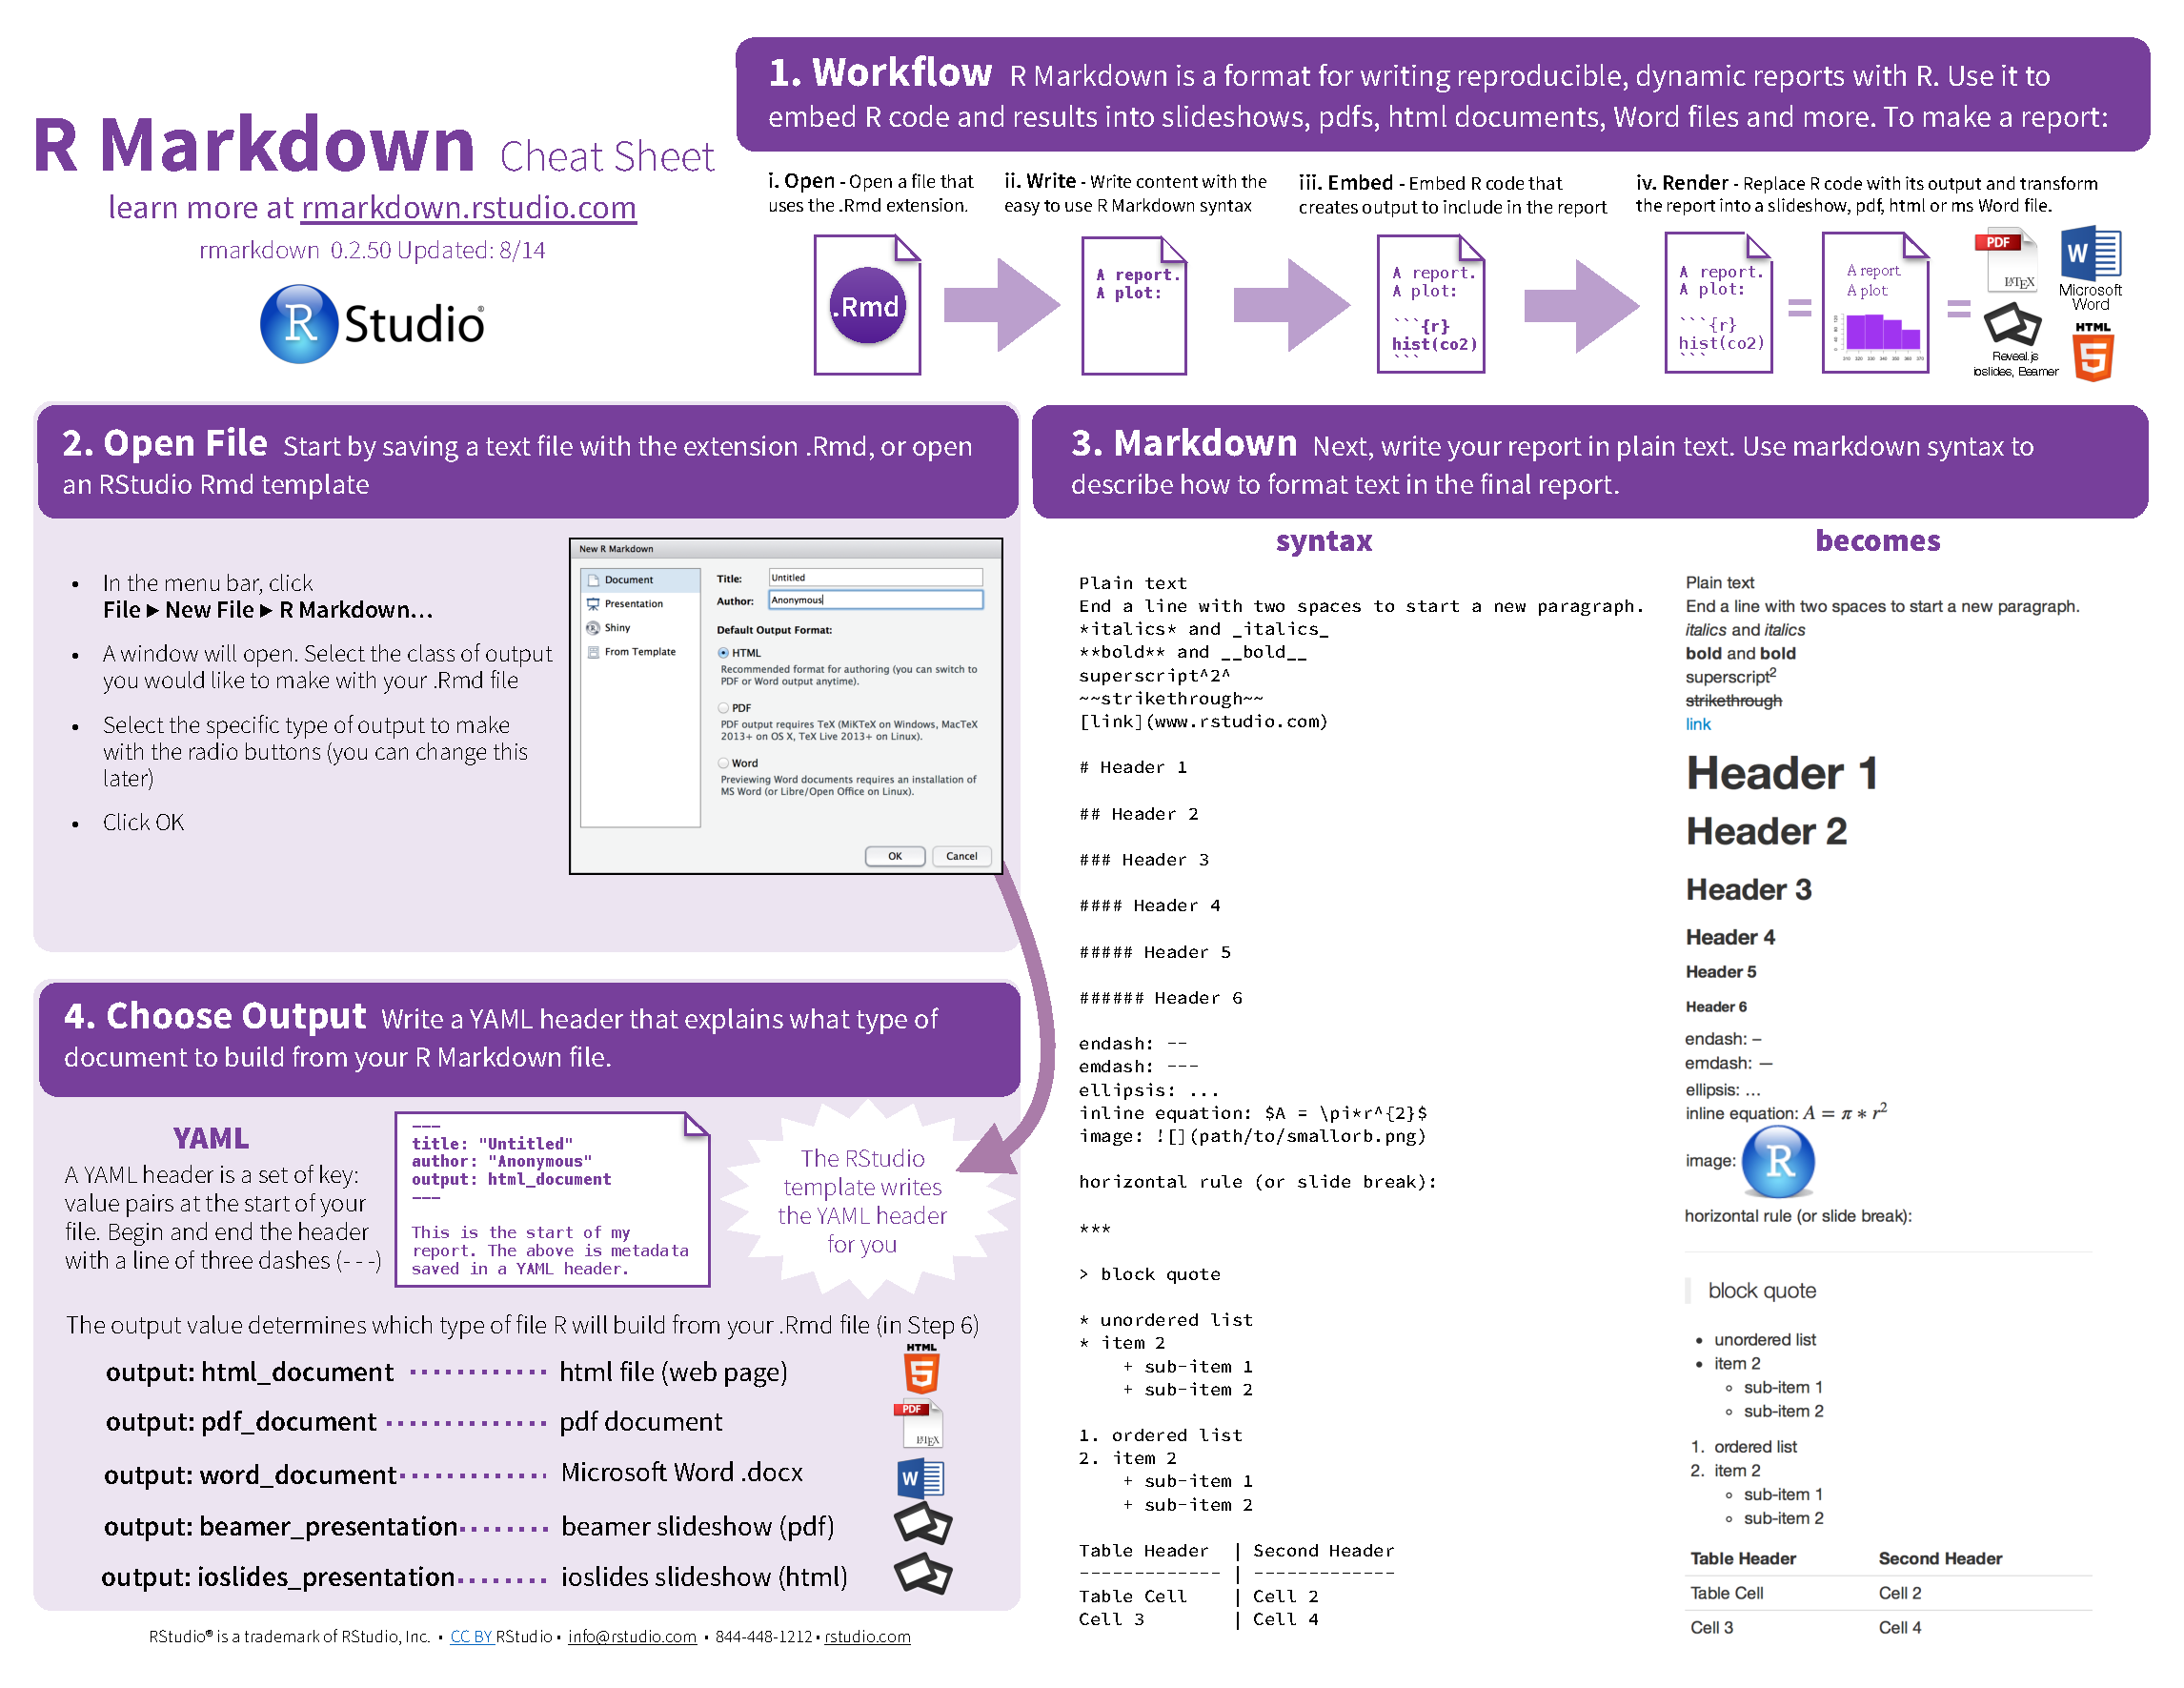
\includegraphics[width=1\textwidth,height=\textheight]{./figures/rmarkdown-cheatsheet.pdf}

\hypertarget{paths-and-folders}{%
\section{Paths and folders}\label{paths-and-folders}}

Your computer stores everything you work with in folders (also called
``directories''). If you open File Explorer on Windows or Finder App on
Mac, you'll see the archive that your computer is storing for you. The
archive has an arrangement which makes it easy to search through your
files -- a tree-like structure. You have a folder, and within that
folder you can have another folder, and within that folder, another
folder, until there is a file. This tree-structure, from root to branch,
is often called a ``path''. For example, the path to your ``myscript.R''
could look something like the structure below:

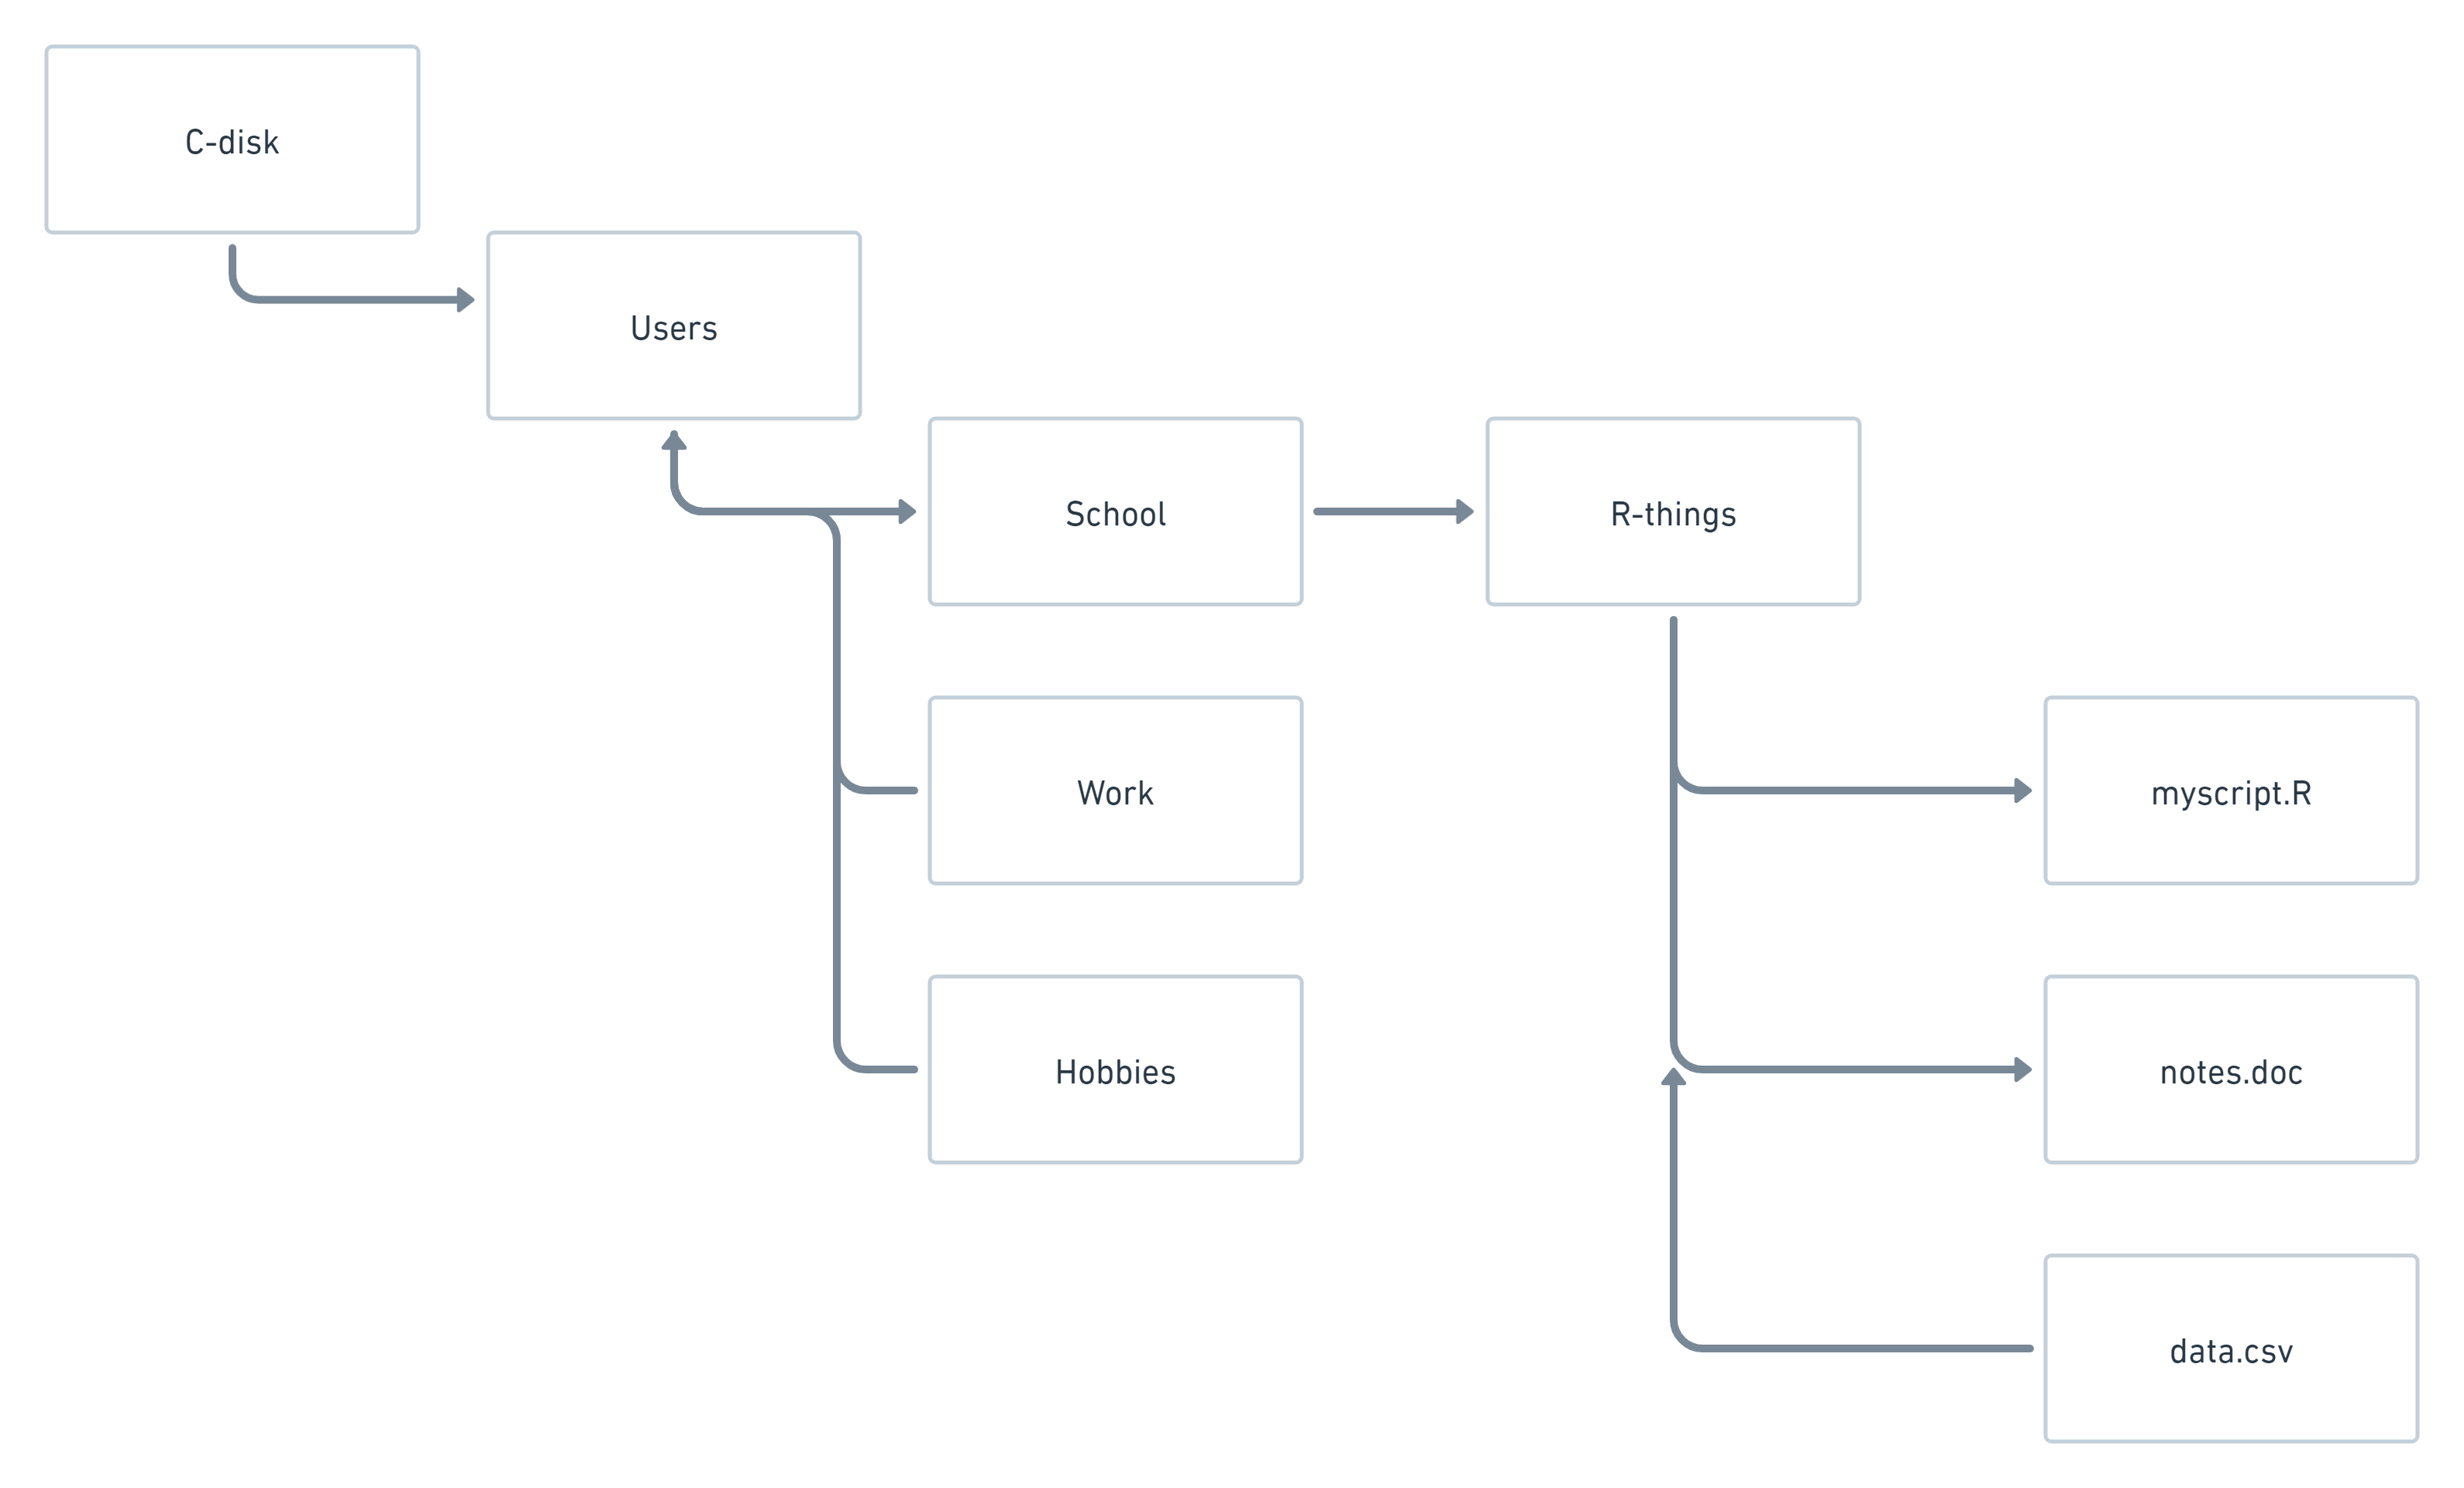
\includegraphics[width=1\textwidth,height=\textheight]{./figures/rfolders.png}
Here, C-disk is the root and the file is myscript.R. The path would be:
C-disk/Users/School/R-things/myscript.R

This is important, because as with any archive, you need to know where
you save things. It's also very important because when we import things
into R, for example a dataset, you need to tell the computer where to
find the file with that dataset. We do that by specifying the path to
the file. For example, if we would want to read data.csv into R, the
code would be:

\begin{Shaded}
\begin{Highlighting}[]
\NormalTok{dataset }\OtherTok{\textless{}{-}} \FunctionTok{read\_csv}\NormalTok{(}\StringTok{"C{-}disk/Users/School/R{-}things/data.csv"}\NormalTok{)}
\end{Highlighting}
\end{Shaded}

Notice that in the code above, \texttt{read\_csv} is the function that
reads a dataset into R, the argument is the path to the file, and we
assign the dataset to an object called ``dataset'' by the
\texttt{dataset\ \textless{}-} part.

Also, notice the suffix on the files. They indicate the type of file we
have. Some examples of file types include:

\begin{itemize}
\tightlist
\item
  \texttt{.R} = Rscript
\item
  \texttt{.Rmd} = R Markdown script
\item
  \texttt{.Rdata} = sata in R-format
\item
  \texttt{.RDS} = a better data format for R
\item
  \texttt{.py} = python scripts
\item
  \texttt{.doc} = Word-file
\item
  \texttt{.csv} = spreadsheet file (data exchange)
\item
  \texttt{.xlsx} = spreadsheet file especially for excel
\item
  \texttt{.txt} = pure text file (notepad)
\item
  \texttt{.json} = JSON-file (data exchange, especially good for nested
  data)
\item
  \texttt{.html} = html file (data exchange or webpages)
\end{itemize}

In RStudio, the window in the right hand corner mirrors the folders on
your computer under the tab ``Files''. You can make adjustments here
just as you can in your folder structure.

\hypertarget{github}{%
\section{Github}\label{github}}

We're going to work in Github. This is a version control space, meaning
that it's a place where you can share your code with others and keep
track of who changes what, when, how, and whether it was a change that
we would really want to keep. It enables you to share your code with the
world, and can be an excellent way to build your CV. Moreover, if you
want to get up and serious with your project, you can integrate Github
with many other platforms such as Amazon and Google Cloud, creating
fluent pipelines for you work. So, there are at least three main
benefits to Github:

\begin{itemize}
\tightlist
\item
  It makes collaboration easier.
\item
  It gives your work exposure and publicity.
\item
  It can be an important component in integration with other platforms.
\end{itemize}

To work in Github, we need to first create a user account. Then, your
team needs to create a repository that can be shared among you. A
repository is a bit like a folder on Github.

\hypertarget{create-a-user-account-for-github}{%
\subsubsection{Create a user account for
Github}\label{create-a-user-account-for-github}}

\begin{enumerate}
\def\labelenumi{\arabic{enumi}.}
\tightlist
\item
  Open \url{https://github.com} in a web browser, and then select Sign
  up.
\item
  Enter your email address.
\item
  Create a password for your new GitHub account, and Enter a username,
  too. Next, choose whether you want to receive updates and
  announcements via email, and then select Continue.
\item
  Verify your account by solving a puzzle. Select the Start Puzzle
  button to do so, and then follow the prompts.
\item
  After you verify your account, select the Create account button.
\item
  Next, GitHub sends a launch code to your email address. Type that
  launch code in the Enter code dialog, and then press Enter.
\item
  GitHub asks you some questions to help tailor your experience. Choose
  the answers that apply to you in the following dialogs:
\end{enumerate}

\begin{itemize}
\tightlist
\item
  How many team members will be working with you?
\item
  What specific features are you interested in using?
\end{itemize}

\begin{enumerate}
\def\labelenumi{\arabic{enumi}.}
\setcounter{enumi}{7}
\tightlist
\item
  On the ``Where teams collaborate and ship'' screen, you can choose
  whether you want to use the Free account or the Team account. To
  choose the Free account, select the Skip personalization button.
\item
  GitHub opens a personalized page in your browser.
\end{enumerate}

\hypertarget{create-a-repository}{%
\subsubsection{Create a repository}\label{create-a-repository}}

\begin{enumerate}
\def\labelenumi{\arabic{enumi}.}
\tightlist
\item
  Click on your profile button in the right hand corner of your Github
  screen and choose ``Your repositories''.
\item
  Click the green button ``New''.
\item
  Type a short, memorable name for your repository.
\item
  Optionally, add a description of your repository.
\item
  Choose a repository visibility. Here, you can pick ``Public''.
\item
  Under ``Initialize this repository with'', choose ``Add a README
  file''.
\item
  Click ``Create repository''.
\end{enumerate}

Now, to add collaborators:

\begin{enumerate}
\def\labelenumi{\arabic{enumi}.}
\tightlist
\item
  Collect the Github usernames for the rest of the team.
\item
  Navigate to the main page of the repository.
\item
  Under your repository name, click Settings.
\item
  In the ``Access'' section of the sidebar, click ``Collaborators''.
\item
  Click ``Add people''.
\end{enumerate}

Once the other collaborators have accepted the invitation to
collaborate, everyone should be able to contribute.

Now, even though we have a shared Github repository, we still work and
code in peace on our own computers. But whenever we make a change in the
code and think it's time to share it with the rest of the team (for
example because we need feedback or because we believe a piece of code
to be done), we can choose to (1) add the change to the Github
repository, (2) commit to the change and (3) push the change. This is
the general flow of working with Github.

How do we add, commit and push a change from our local computer to the
Github repository? By cloning the repository to our computer. This is
possible to do in the terminal, but we will here show you how to do it
in RStudio.

\hypertarget{github-and-rstudio}{%
\subsection{Github and RStudio}\label{github-and-rstudio}}

Github can work with many platforms, including RStudio! To get there,
however, the first thing we need to do is to install git, the system
that allows us to work with Github from our computer. So Github is the
version control \textbf{space}, and git is the version control
\textbf{system}. Git can be downloaded from here:
\url{http://git-scm.com/downloads}

Once you've installed git, you'll need to activate it in RStudio:

\begin{enumerate}
\def\labelenumi{\arabic{enumi}.}
\tightlist
\item
  Find the Tools menu in the top of the RStudio interface and go to
  Global Options.
\item
  Click Git/SVN.
\item
  Click Enable version control interface for RStudio projects.
\item
  Under ``Git executable'', if there is no path there, enter the path
  for your the git file that you downloaded earlier.
\end{enumerate}

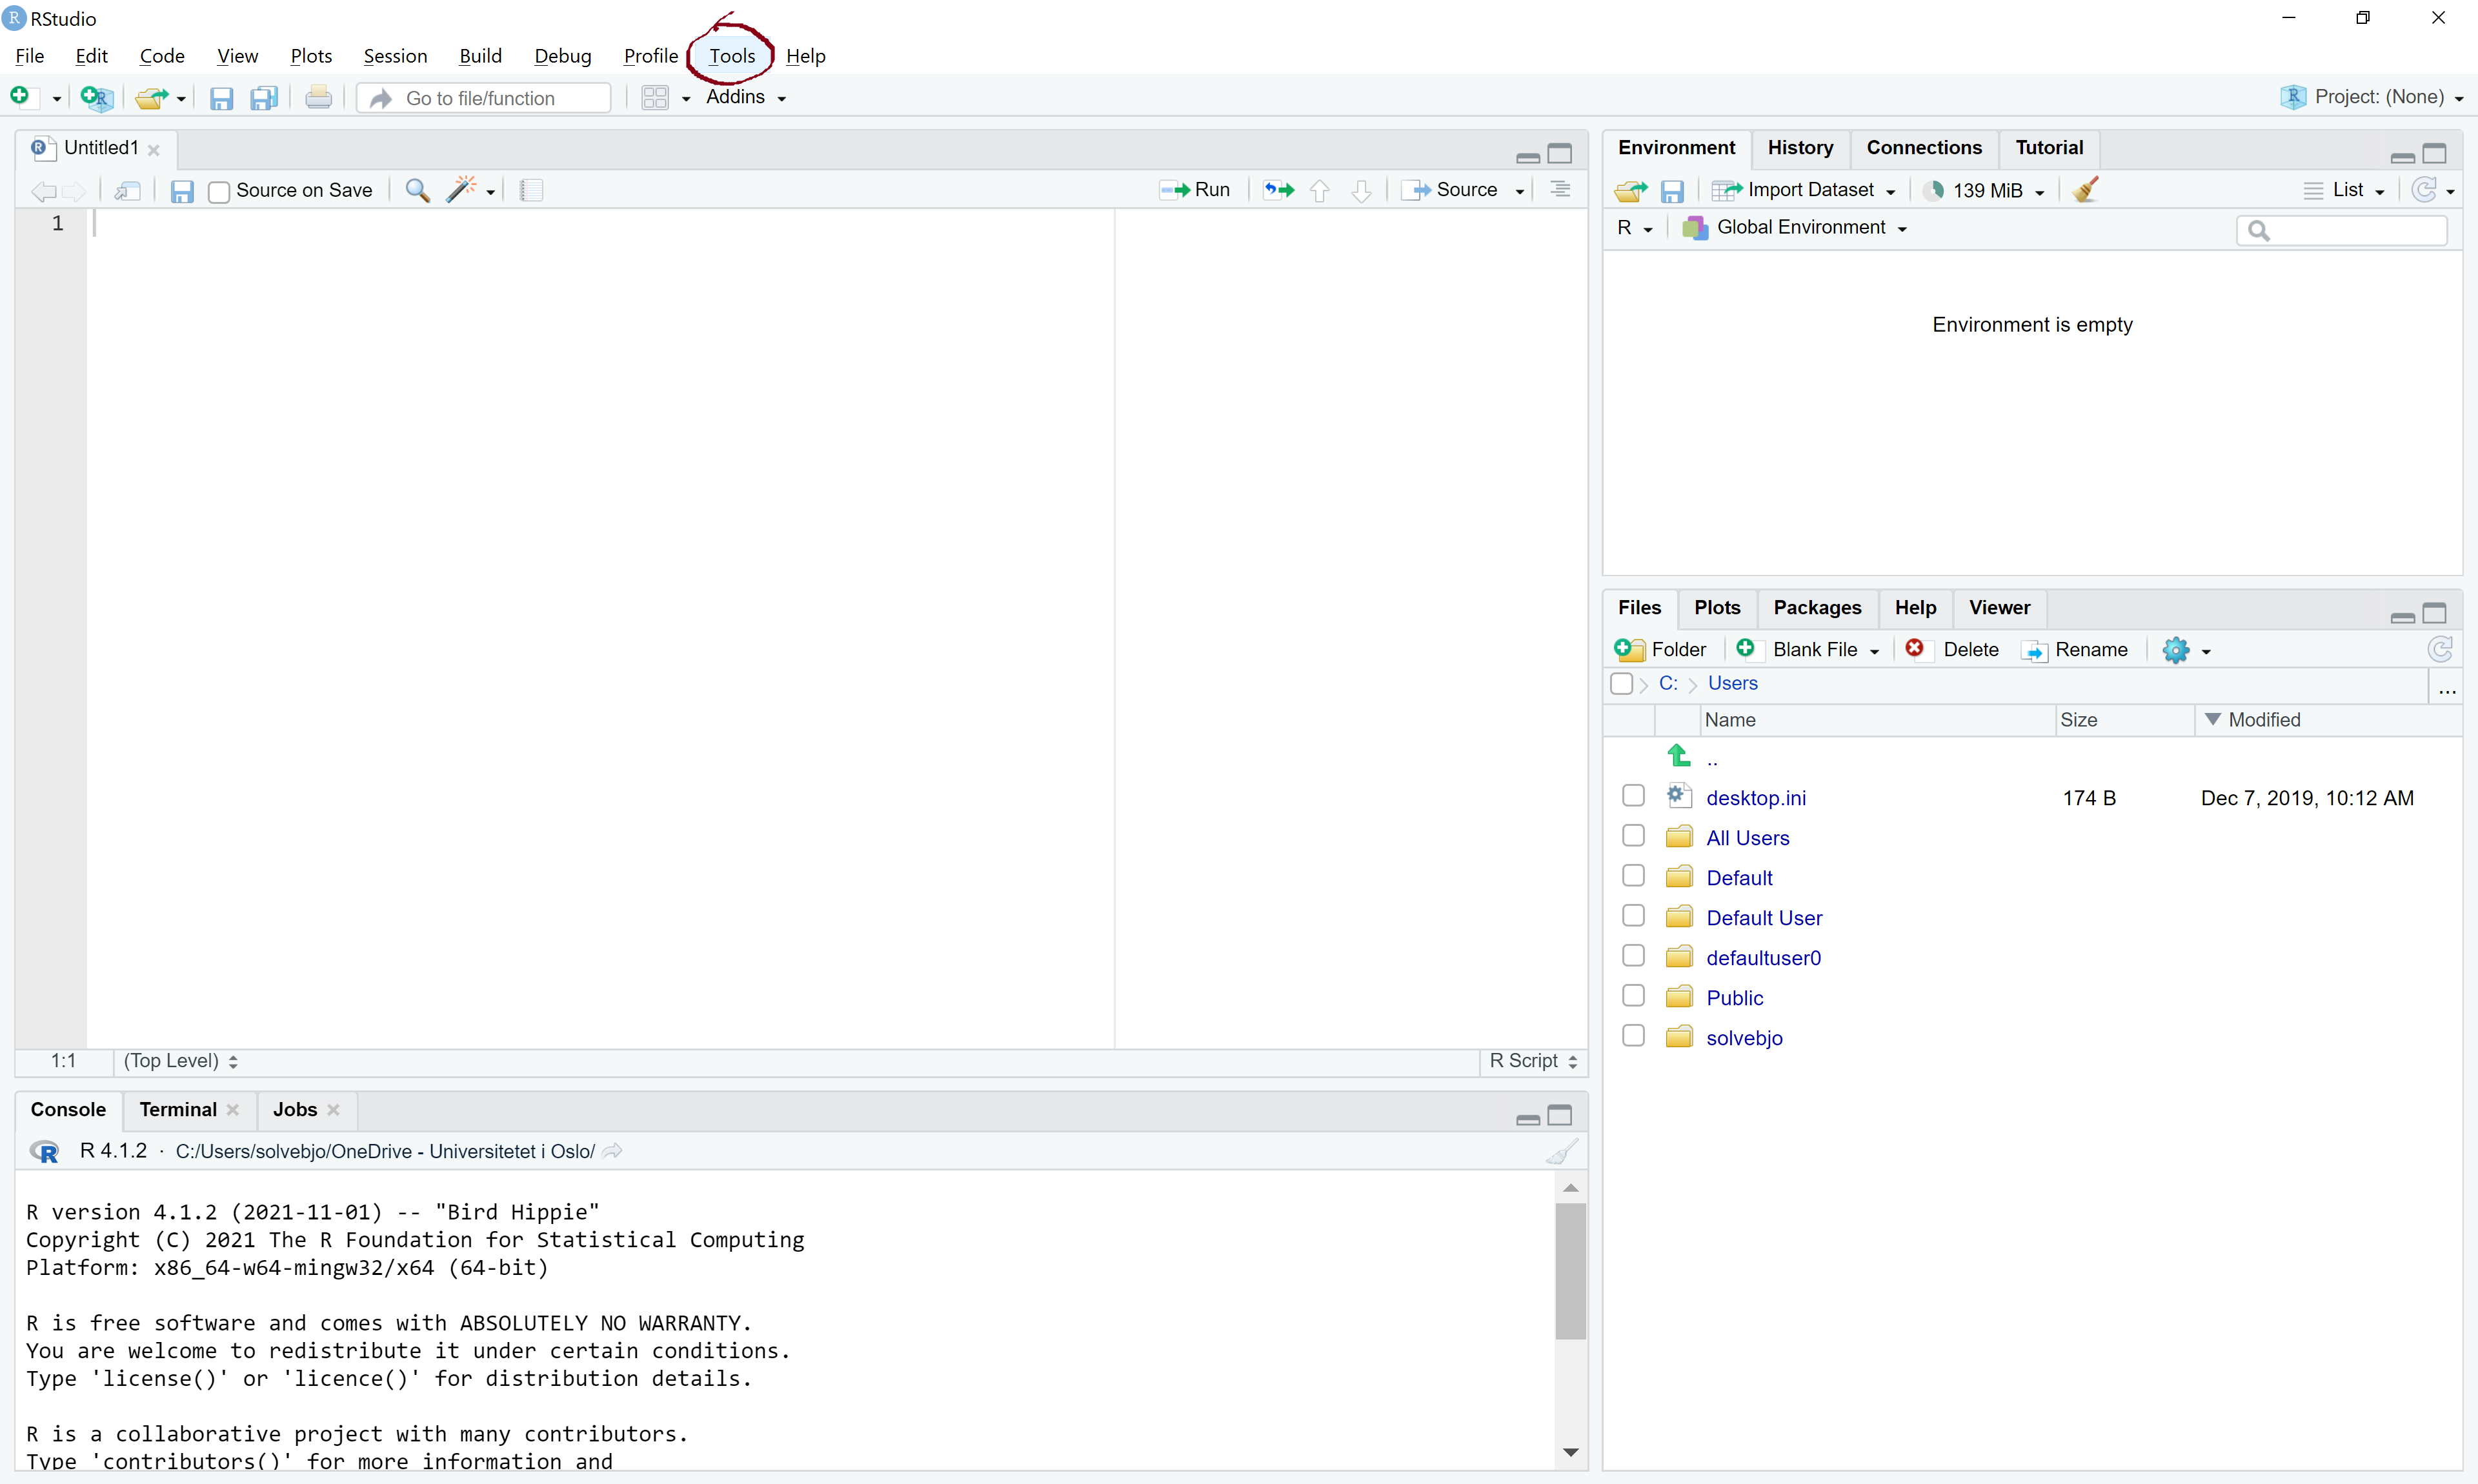
\includegraphics[width=0.8\textwidth,height=\textheight]{./figures/git1.png}
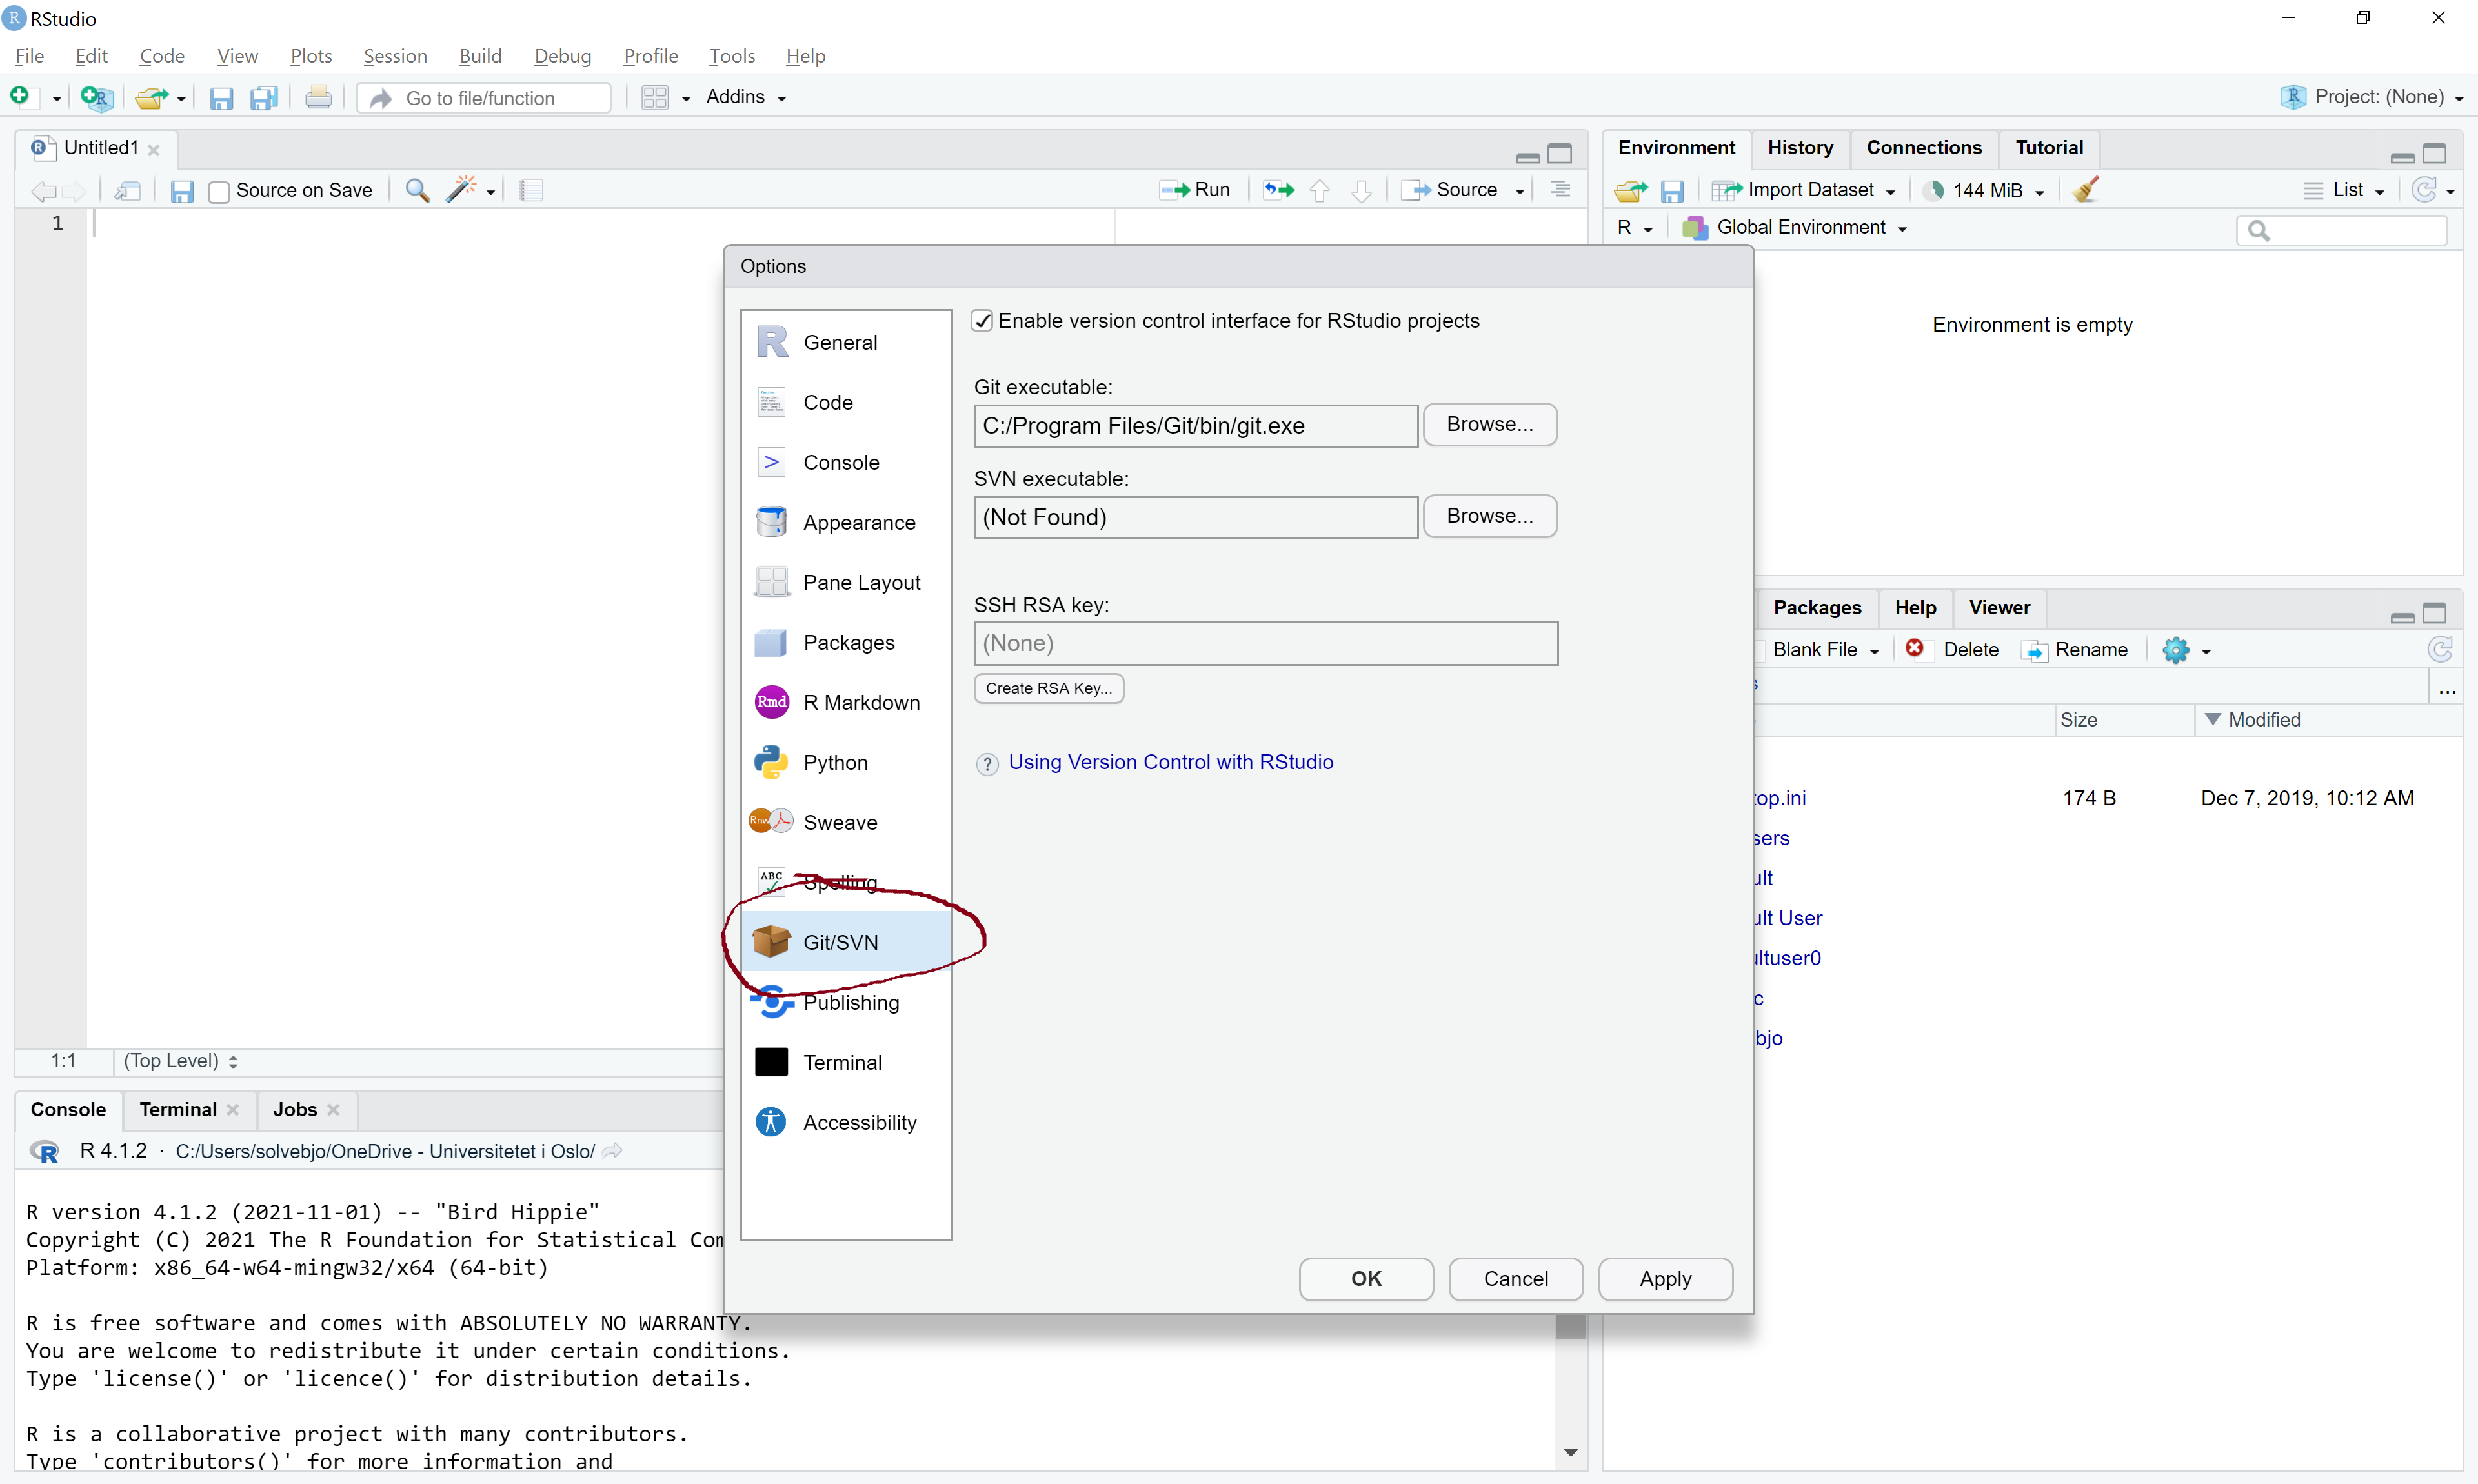
\includegraphics[width=0.8\textwidth,height=\textheight]{./figures/git2.png}
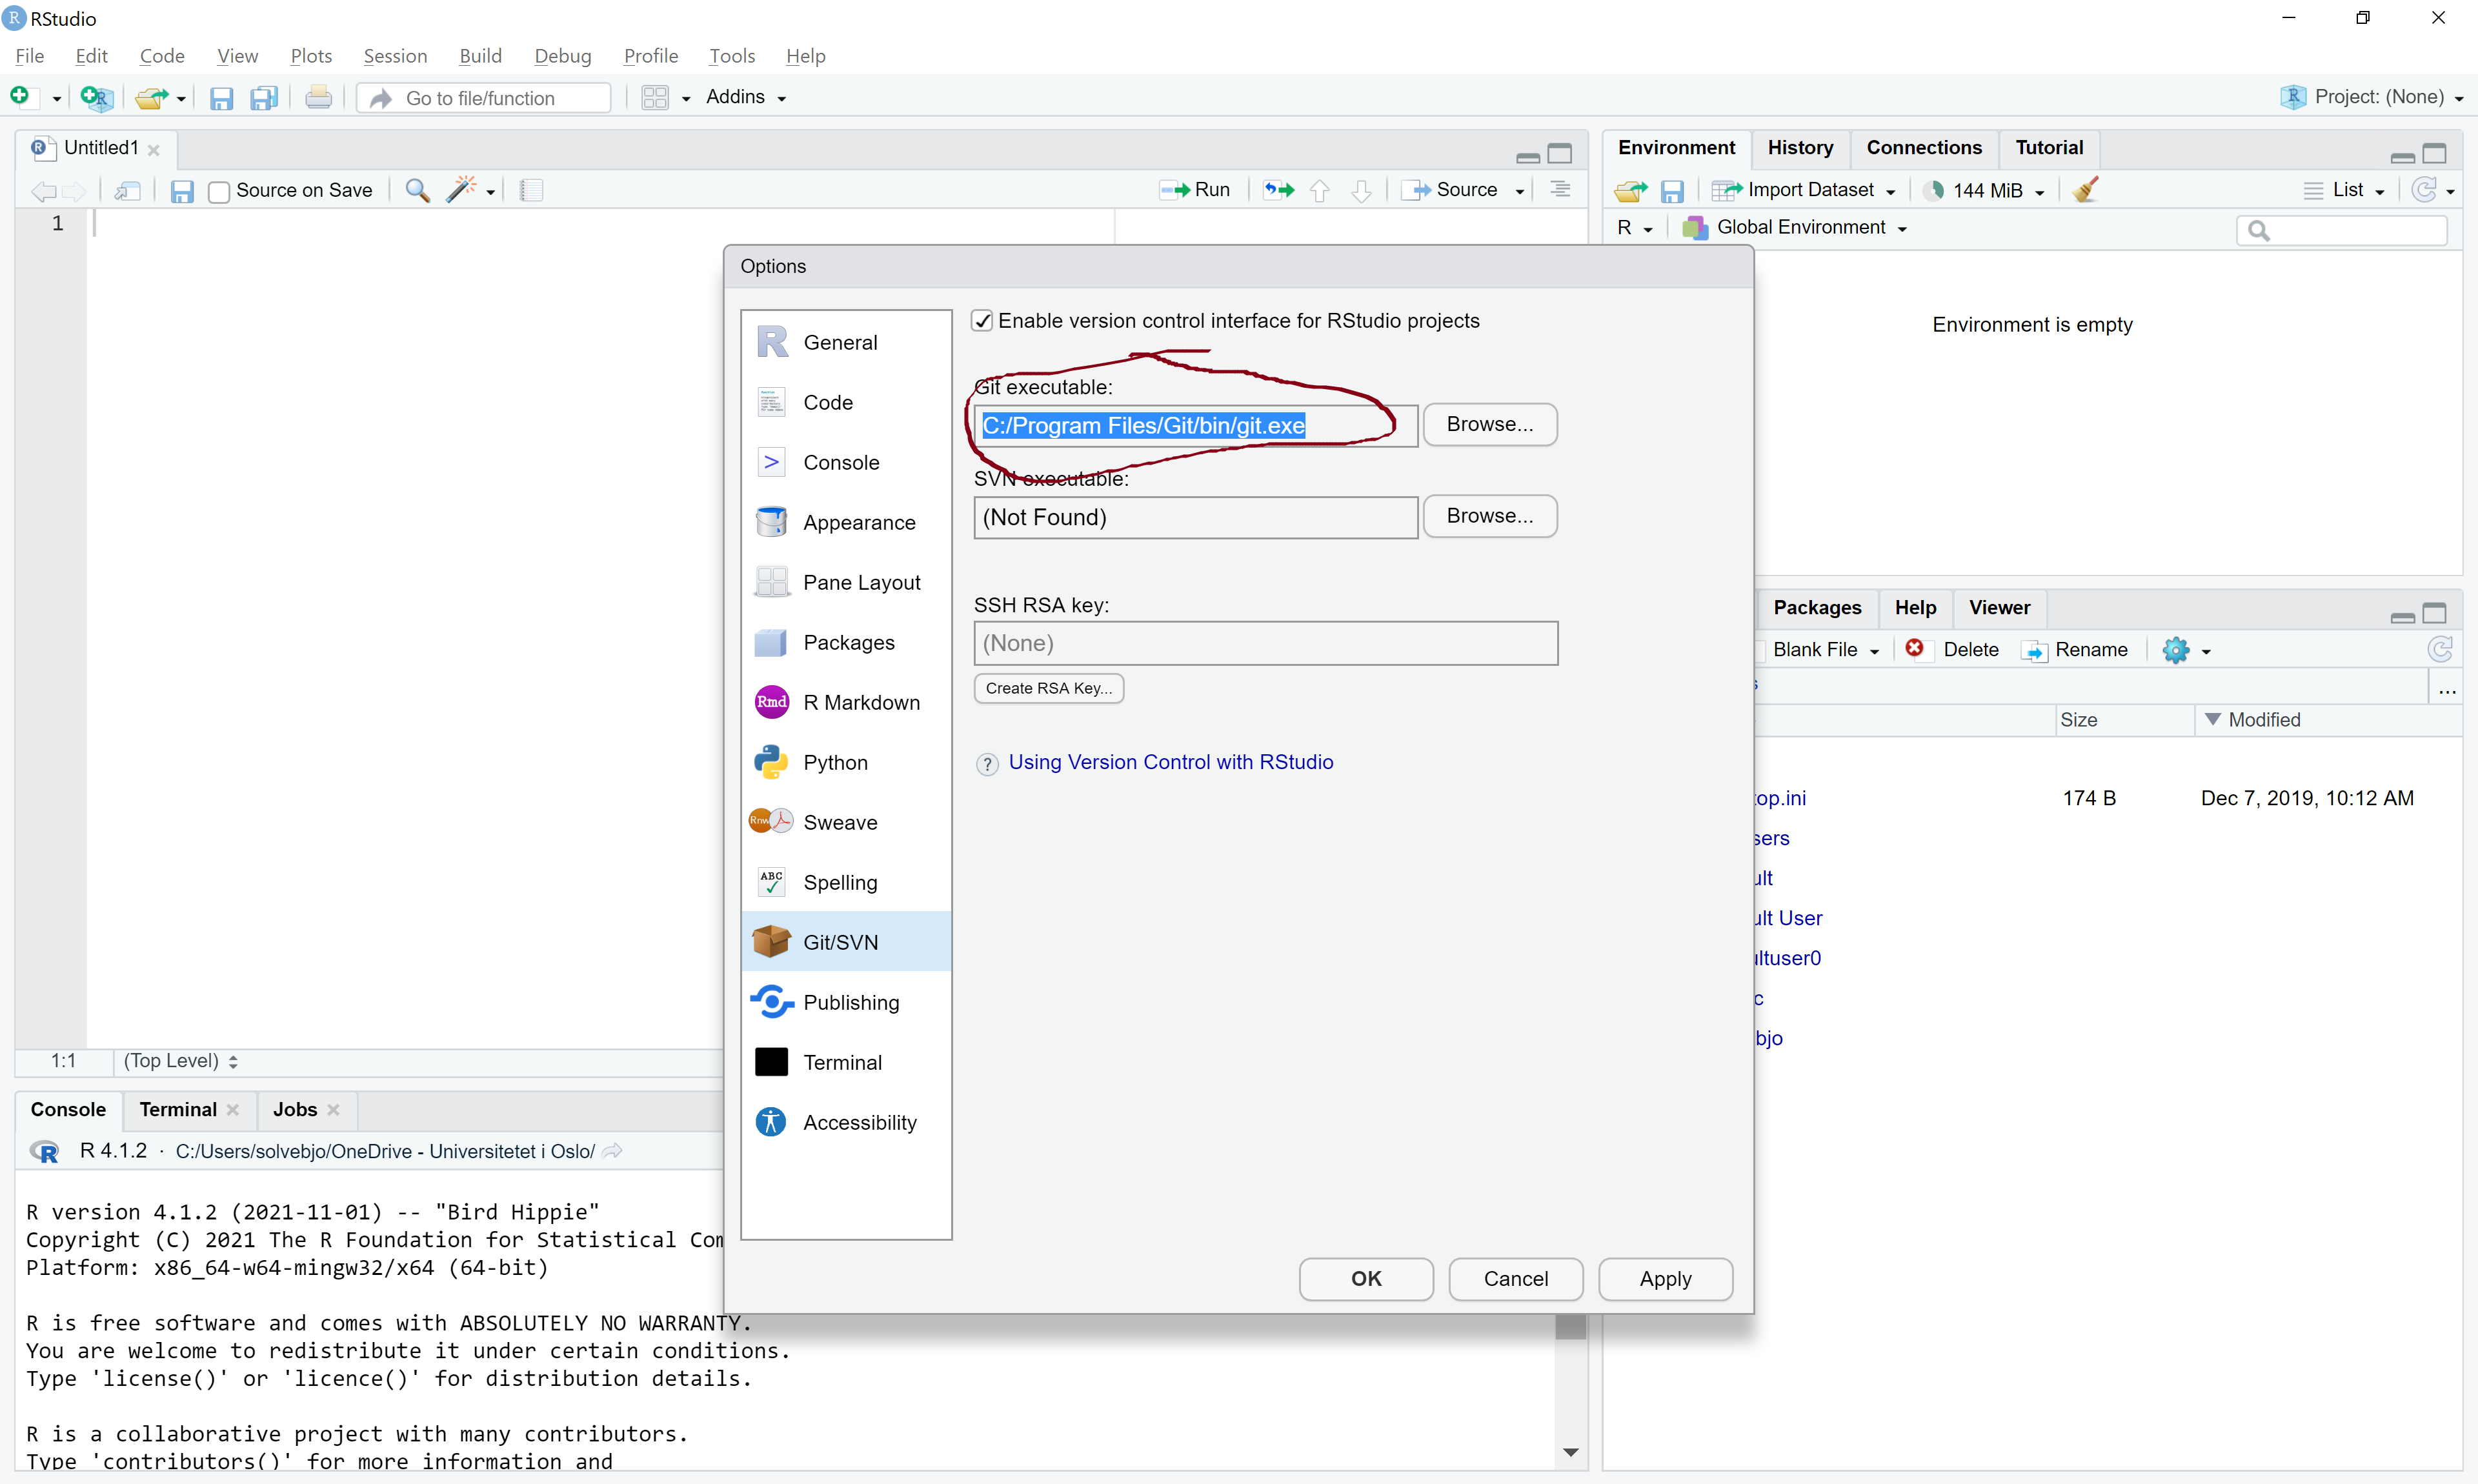
\includegraphics[width=0.8\textwidth,height=\textheight]{./figures/git3.png}

When this is up and working, we need to use our newly installed git to
do the actual cloning the Github repository to our own computer. To do
this, you need to create a new project in RStudio that is tied to the
repository. This is how to do that:

\begin{enumerate}
\def\labelenumi{\arabic{enumi}.}
\tightlist
\item
  Under ``File'' in the upper left hand corner of your RStudio, choose
  ``New project''. Alteratively, click on the icon of an R in a box with
  a green plus sign.
\end{enumerate}

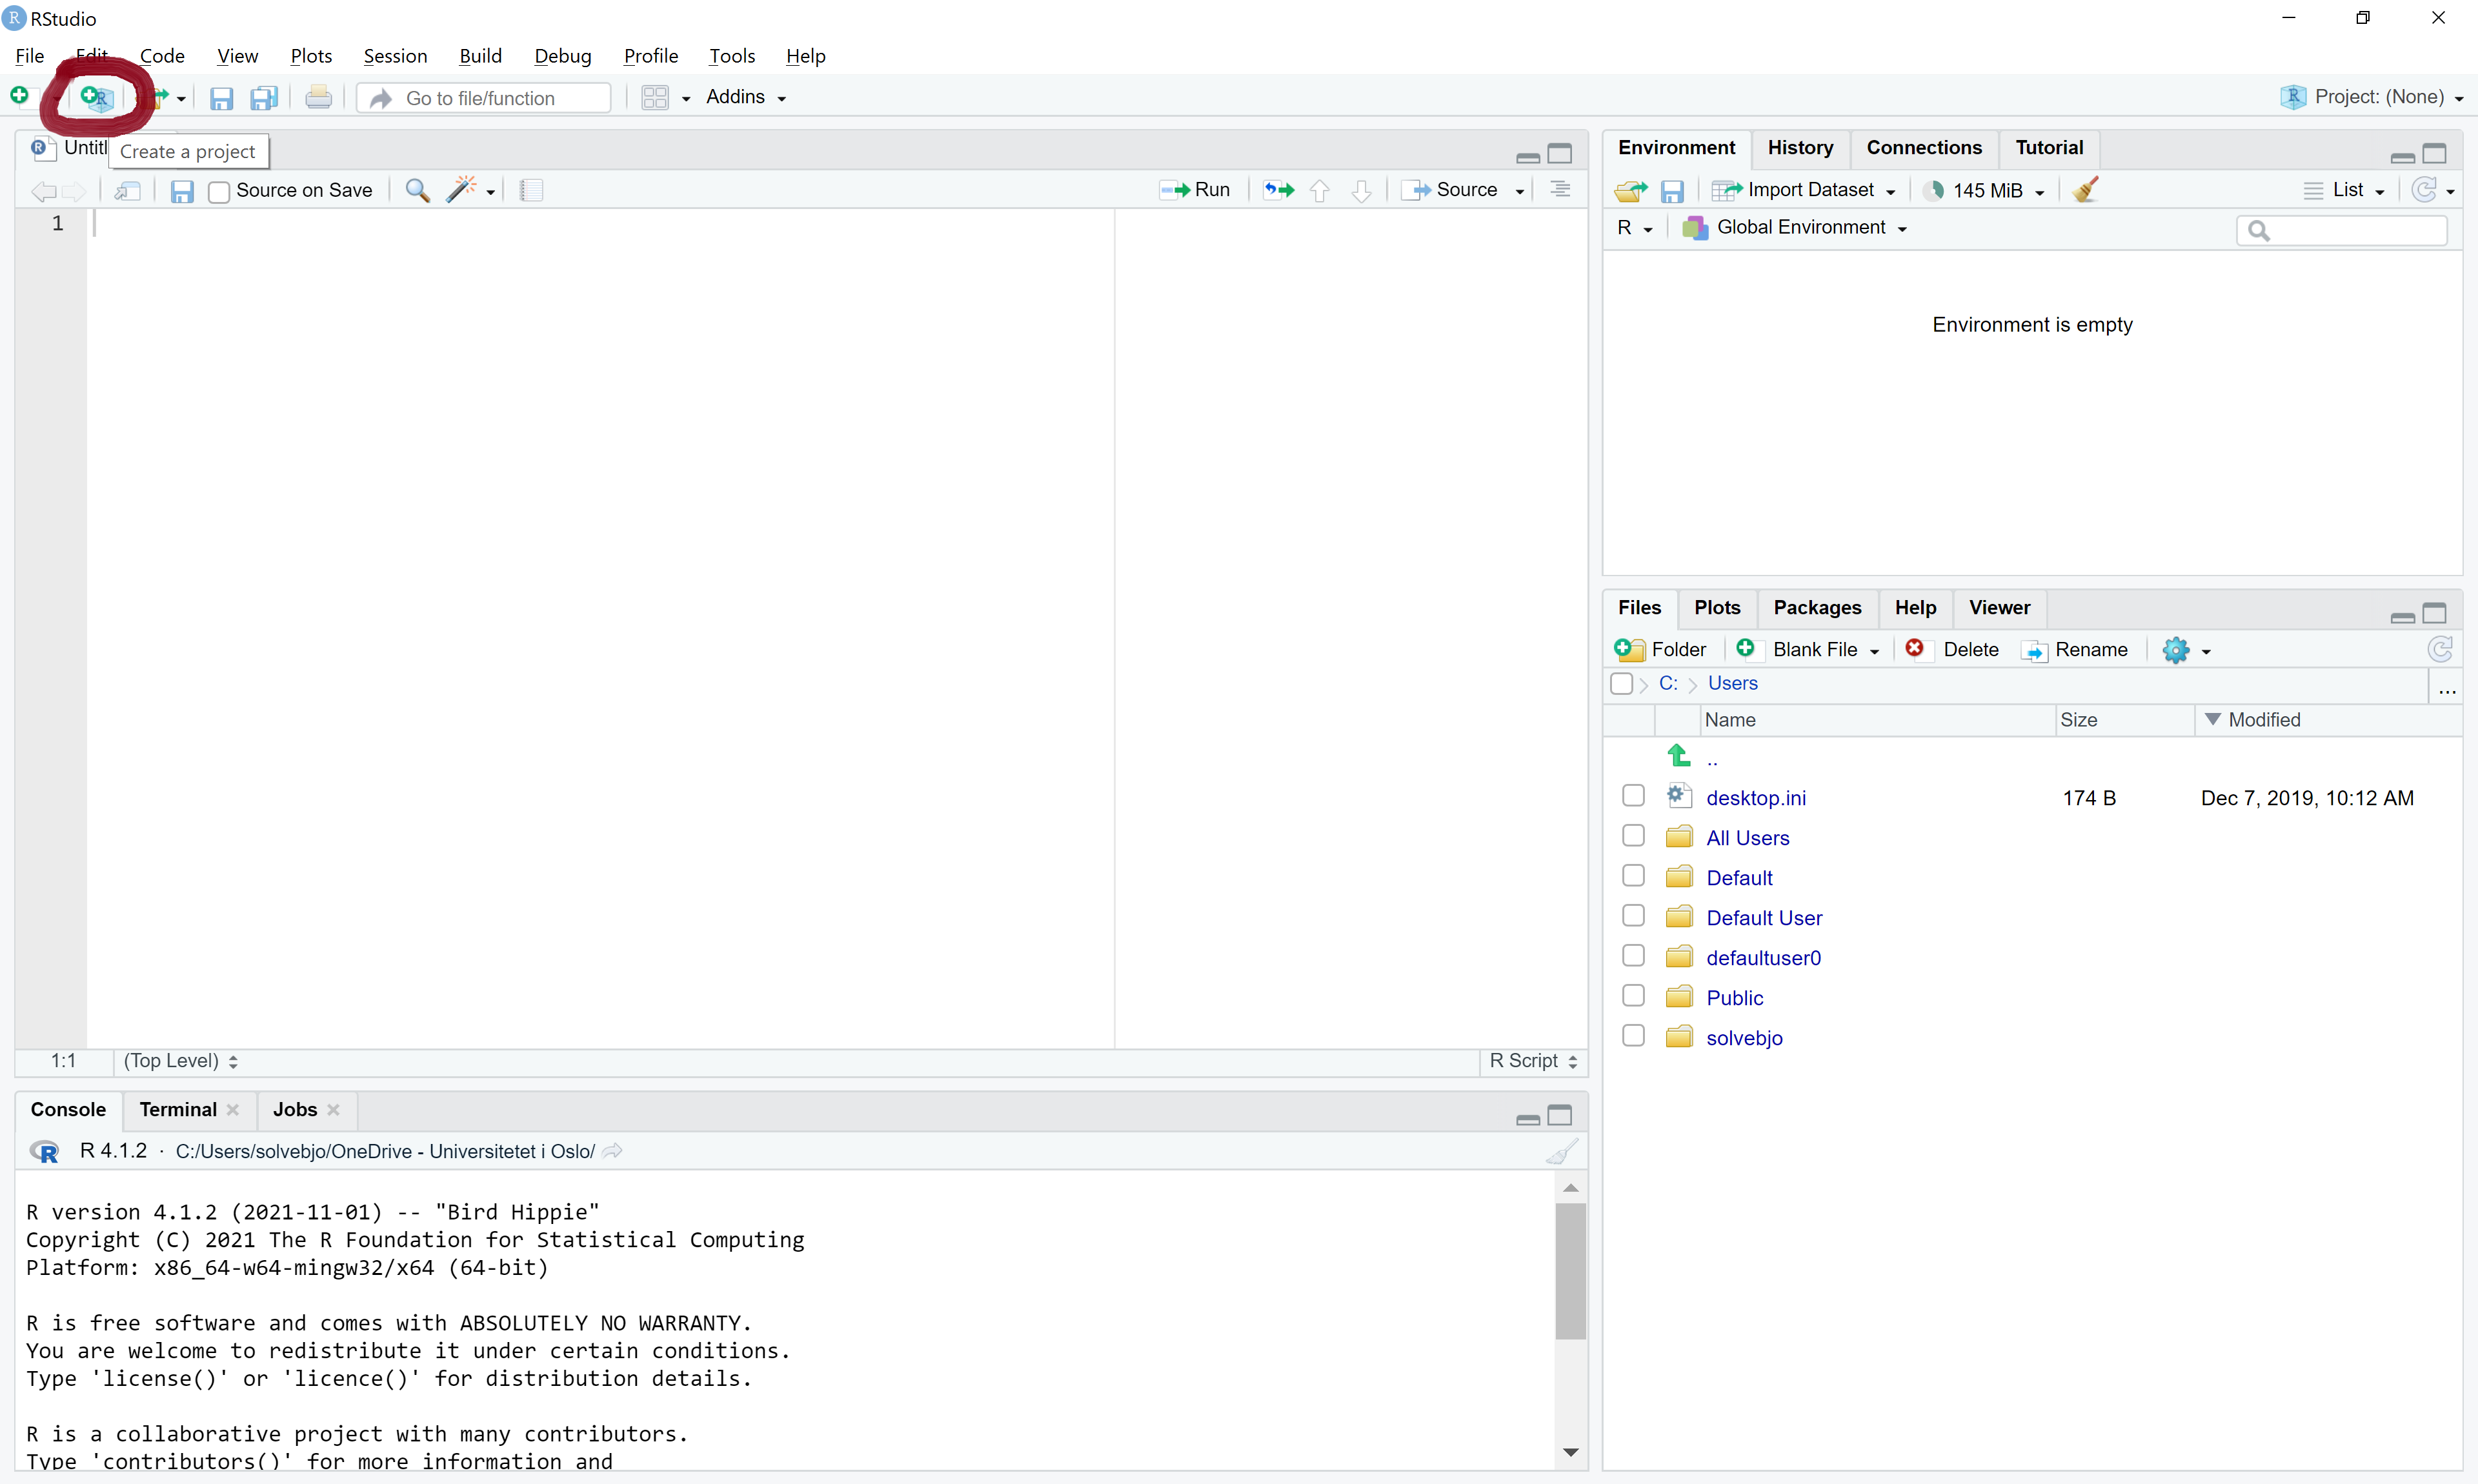
\includegraphics[width=0.8\textwidth,height=\textheight]{./figures/project1.png}

\begin{enumerate}
\def\labelenumi{\arabic{enumi}.}
\setcounter{enumi}{1}
\tightlist
\item
  Choose ``Version Control''.
\end{enumerate}

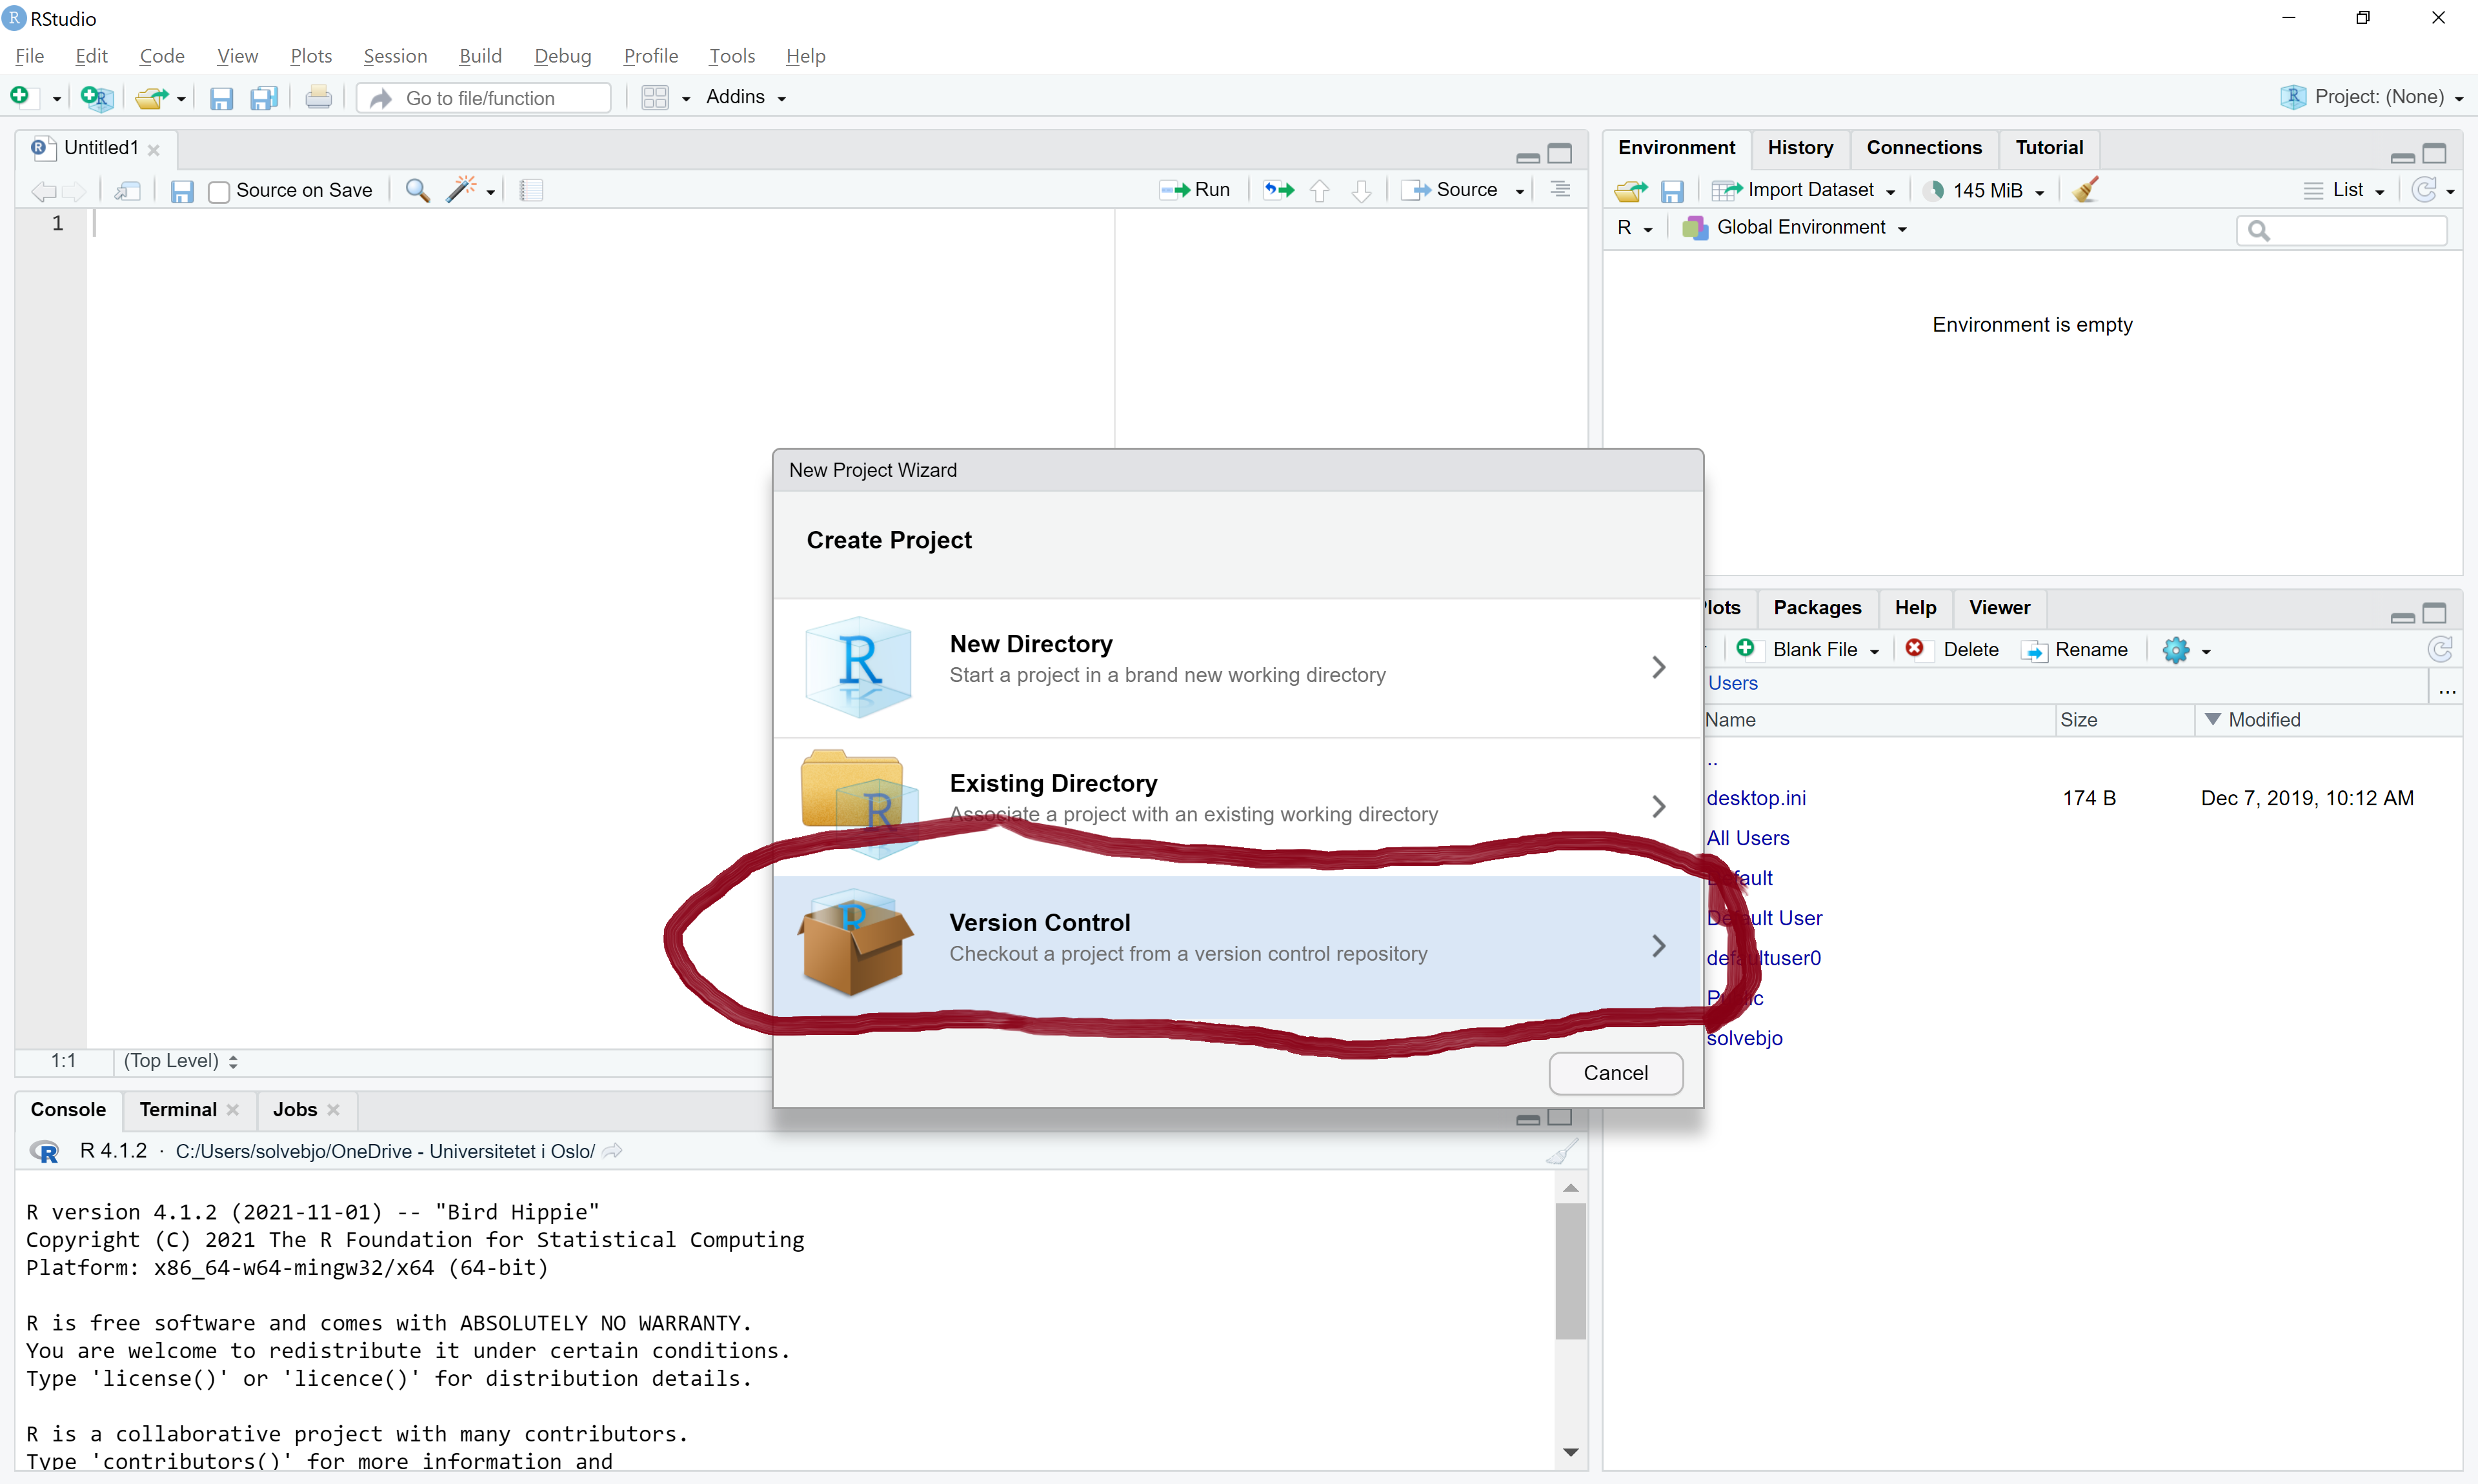
\includegraphics[width=0.8\textwidth,height=\textheight]{./figures/project2.png}

\begin{enumerate}
\def\labelenumi{\arabic{enumi}.}
\setcounter{enumi}{2}
\tightlist
\item
  Choose ``Git''.
\end{enumerate}

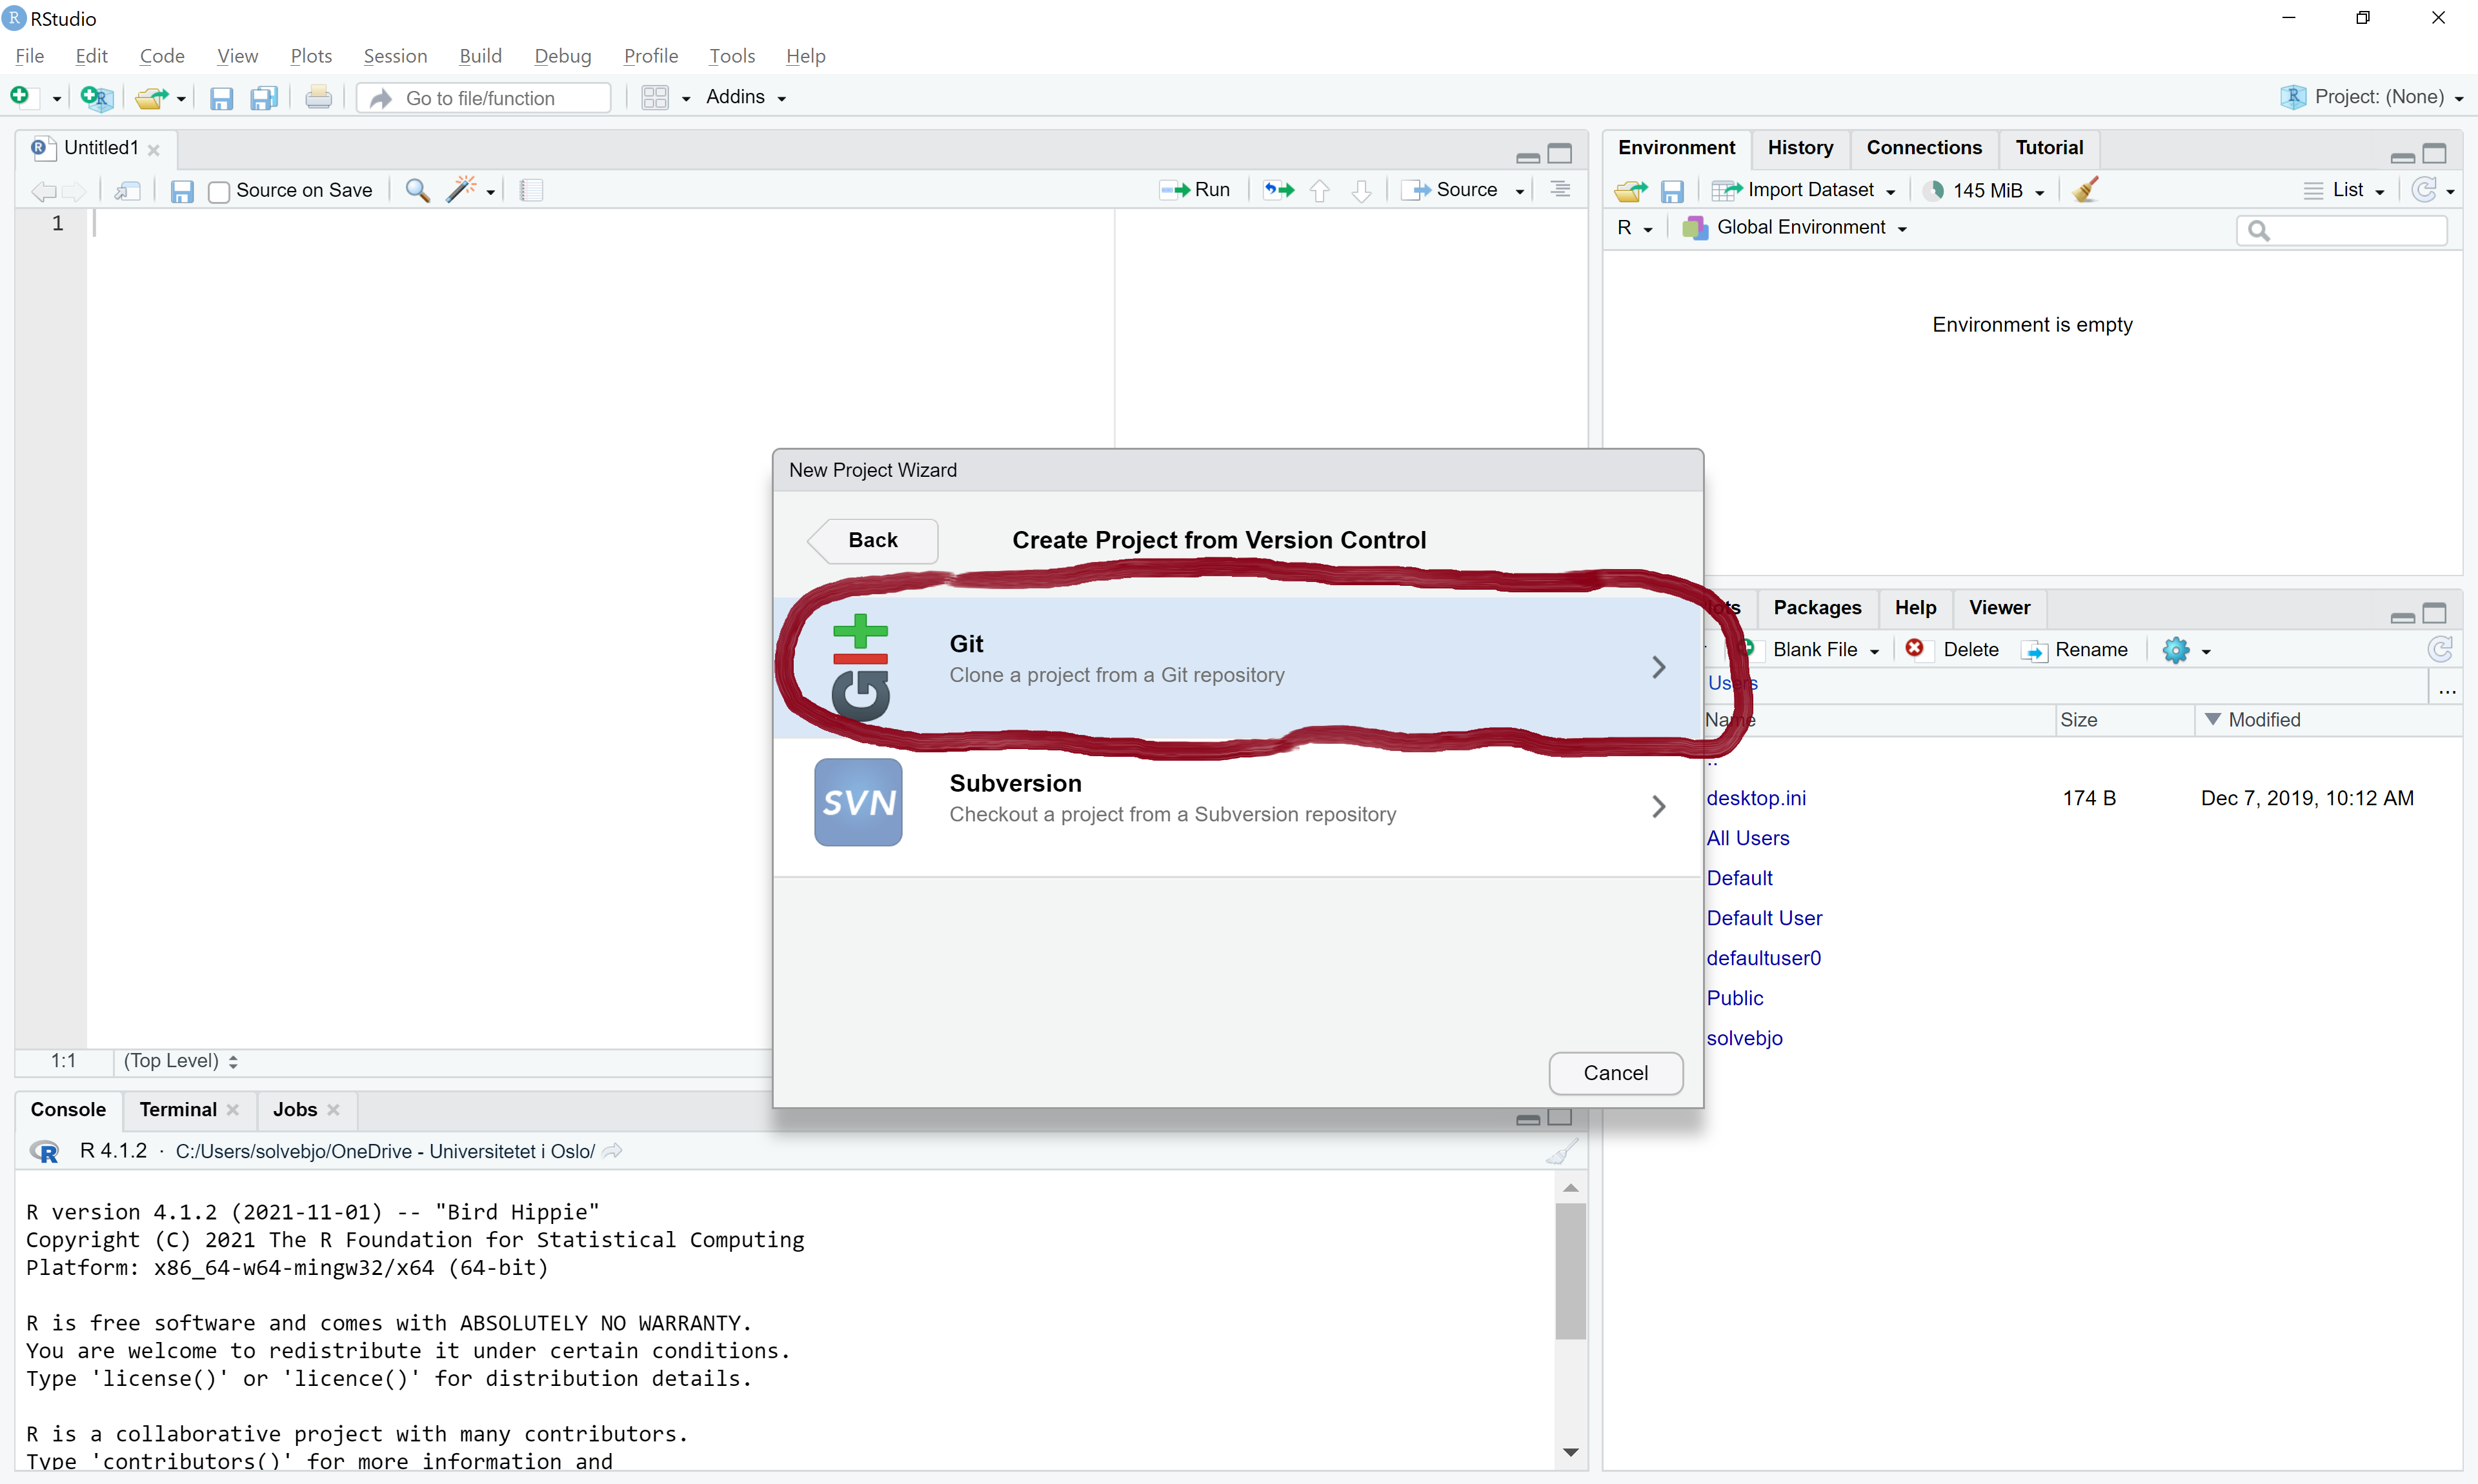
\includegraphics[width=0.8\textwidth,height=\textheight]{./figures/project3.png}

\begin{enumerate}
\def\labelenumi{\arabic{enumi}.}
\setcounter{enumi}{3}
\tightlist
\item
  Here, you are asked for the Repository URL. To find that, go back to
  the main page in your Repository in Github, and click on the green
  ``Code'' button. Copy the URL-path shown there. Then, paste it into
  the space for your Repository URL in RStudio.
\end{enumerate}

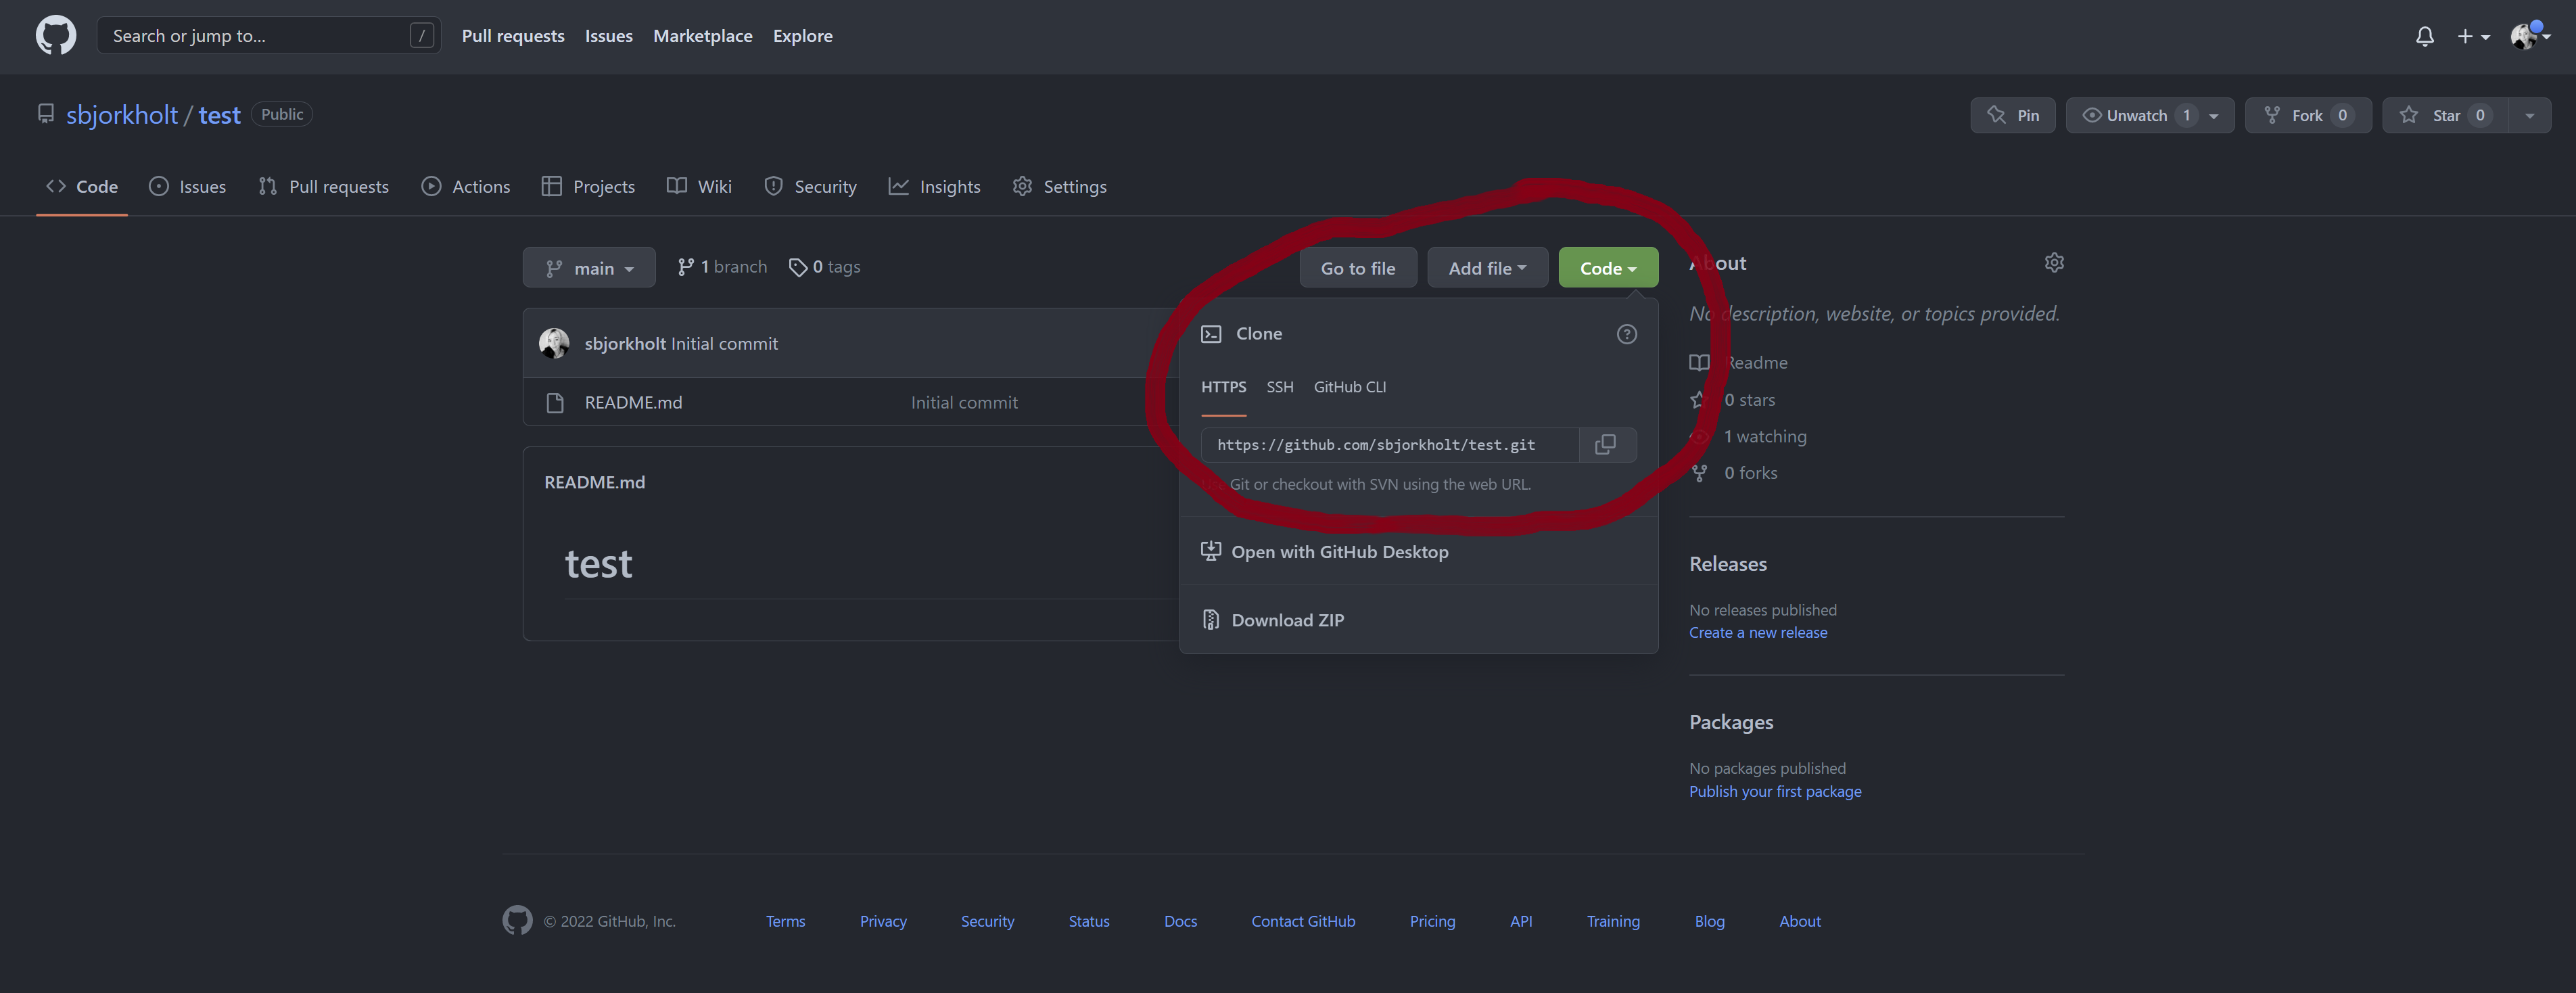
\includegraphics[width=0.8\textwidth,height=\textheight]{./figures/project4.png}
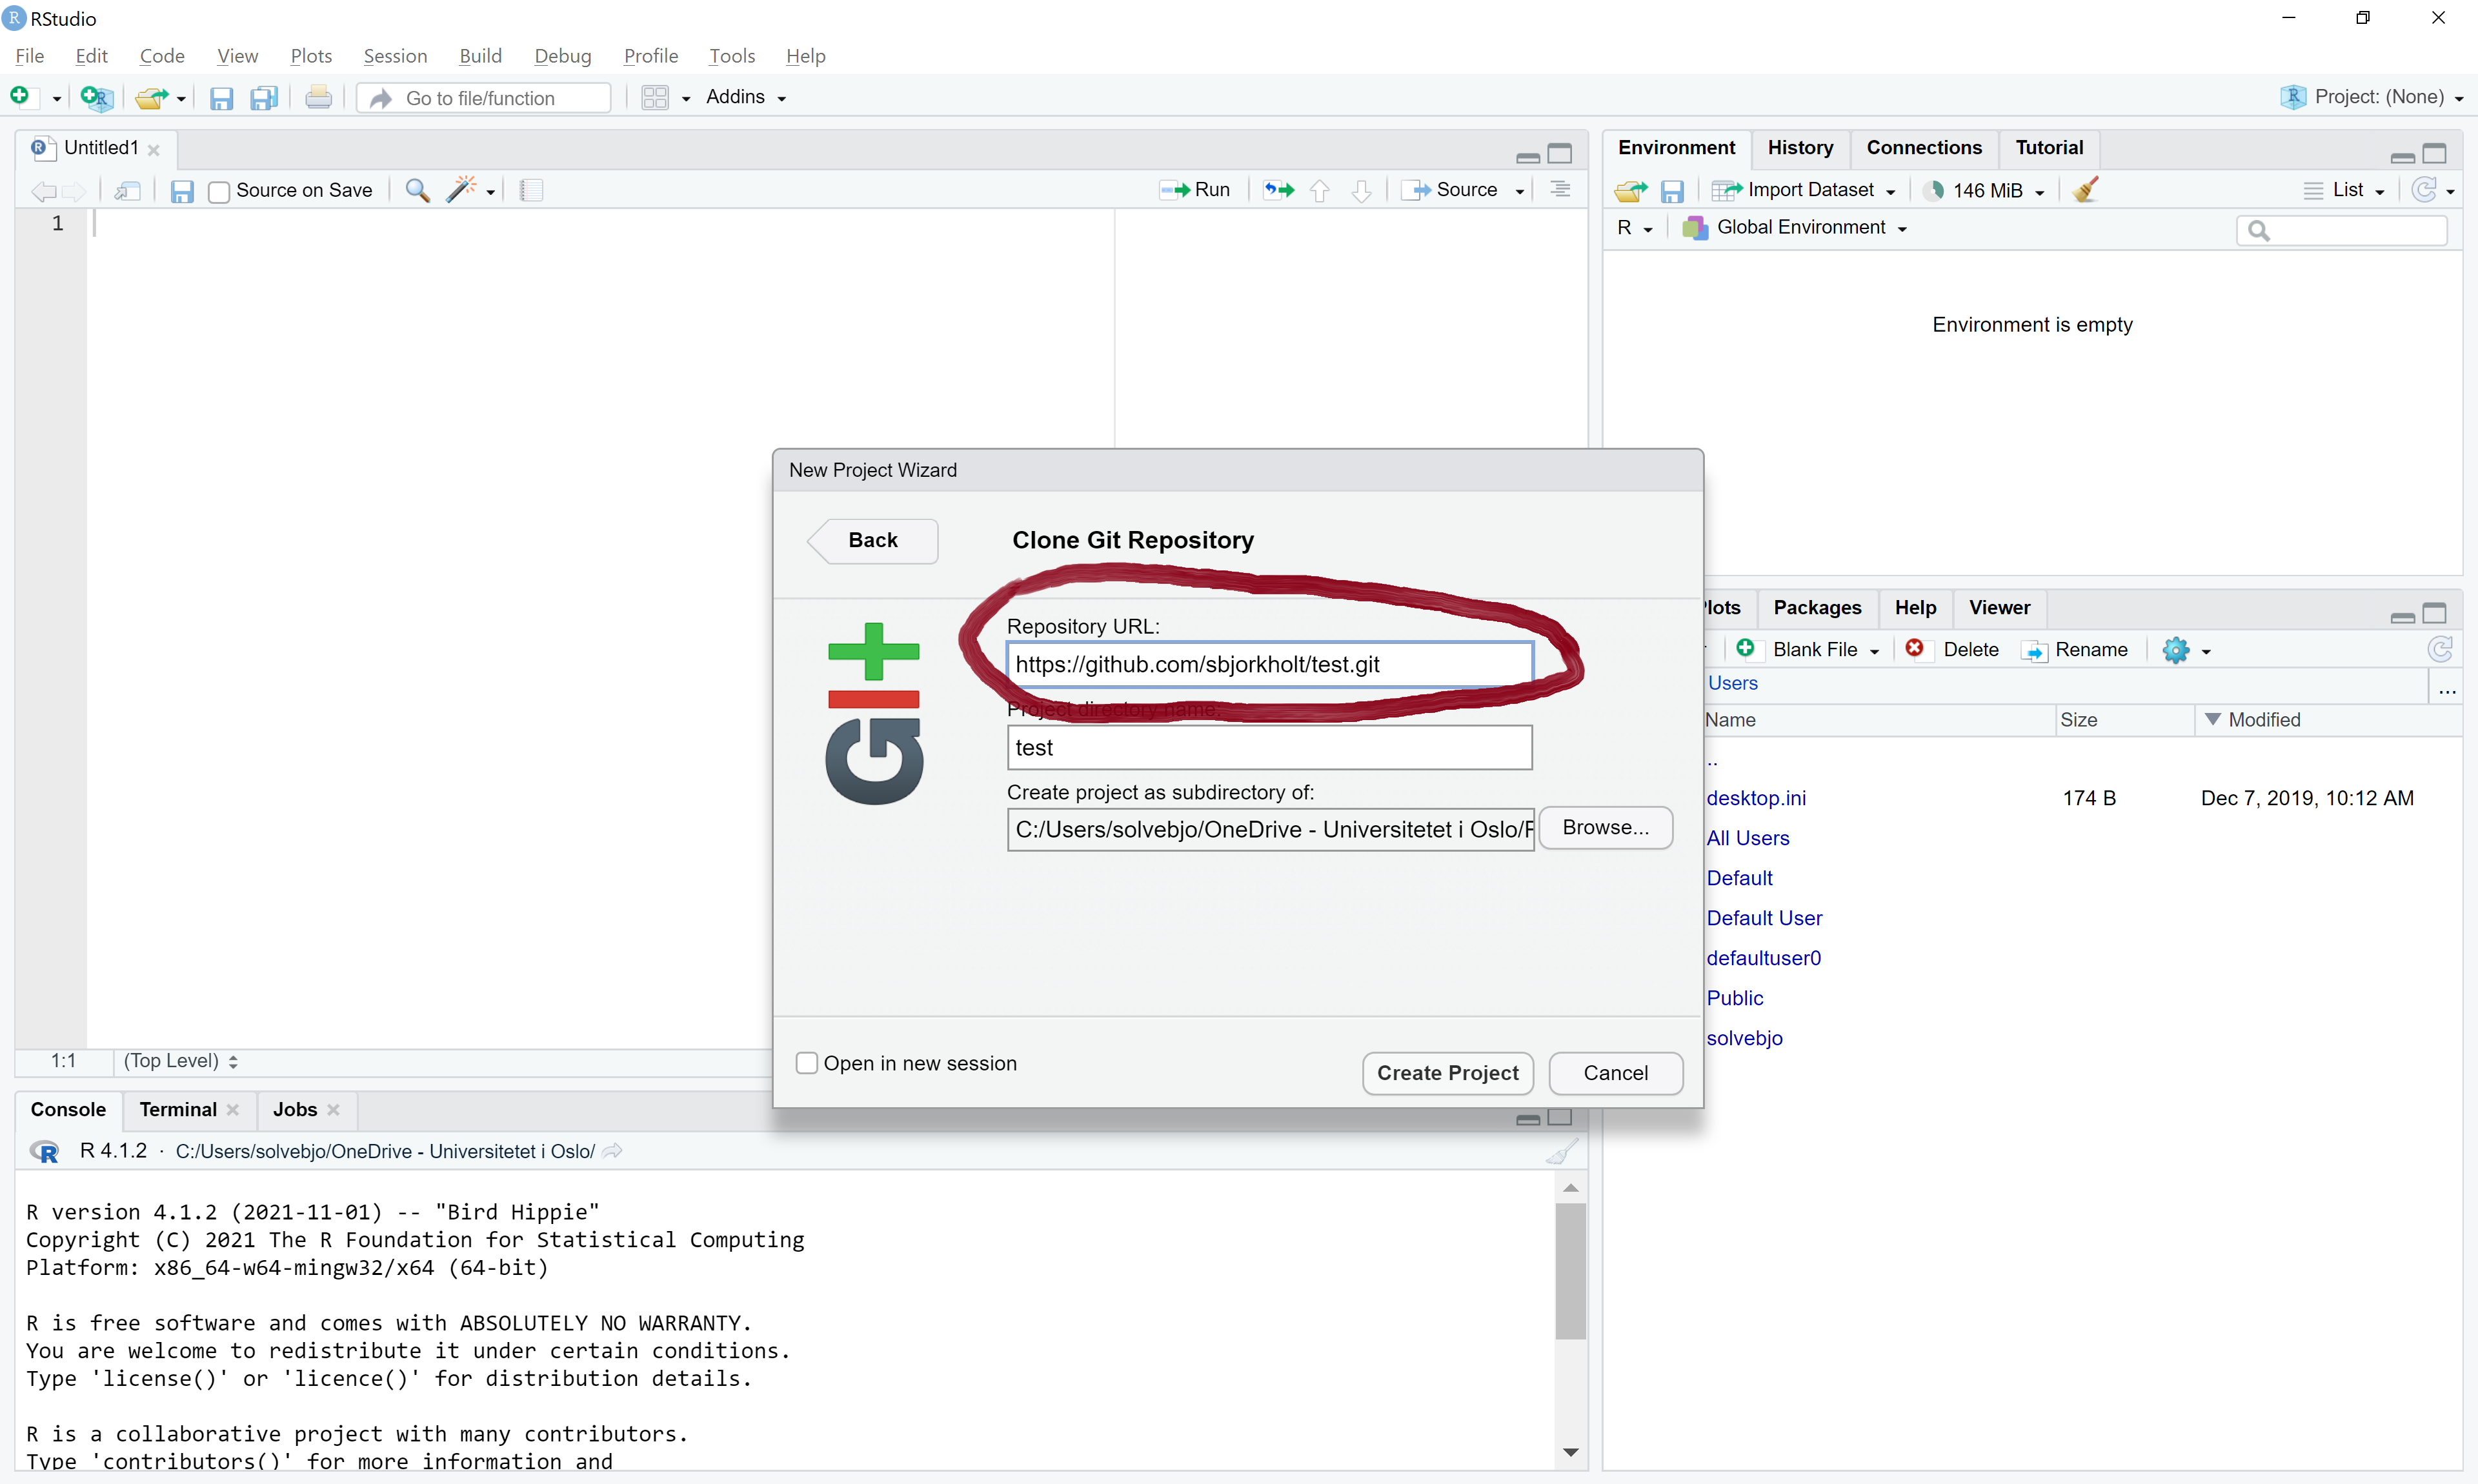
\includegraphics[width=0.8\textwidth,height=\textheight]{./figures/project5.png}

\begin{enumerate}
\def\labelenumi{\arabic{enumi}.}
\setcounter{enumi}{4}
\tightlist
\item
  Use the ``Browse'' button to choose where on your computer you want to
  place your folder. It should be a place you can easily find again. And
  it should not be under ``Downloads''. Recall that a Repository in
  Github is kind of like a folder, so when you clone the repository like
  this, you will create a folder on your computer that matches the
  folder on Github.
\end{enumerate}

And now, you've successfully cloned the Github repository to your own
computer. In the upper right hand corner of your Rstudio, there is now a
tab called ``Git''. Moreover, in the bottom right hand corner, under
``Files'', you find the folder on your computer which matches the Github
repository.

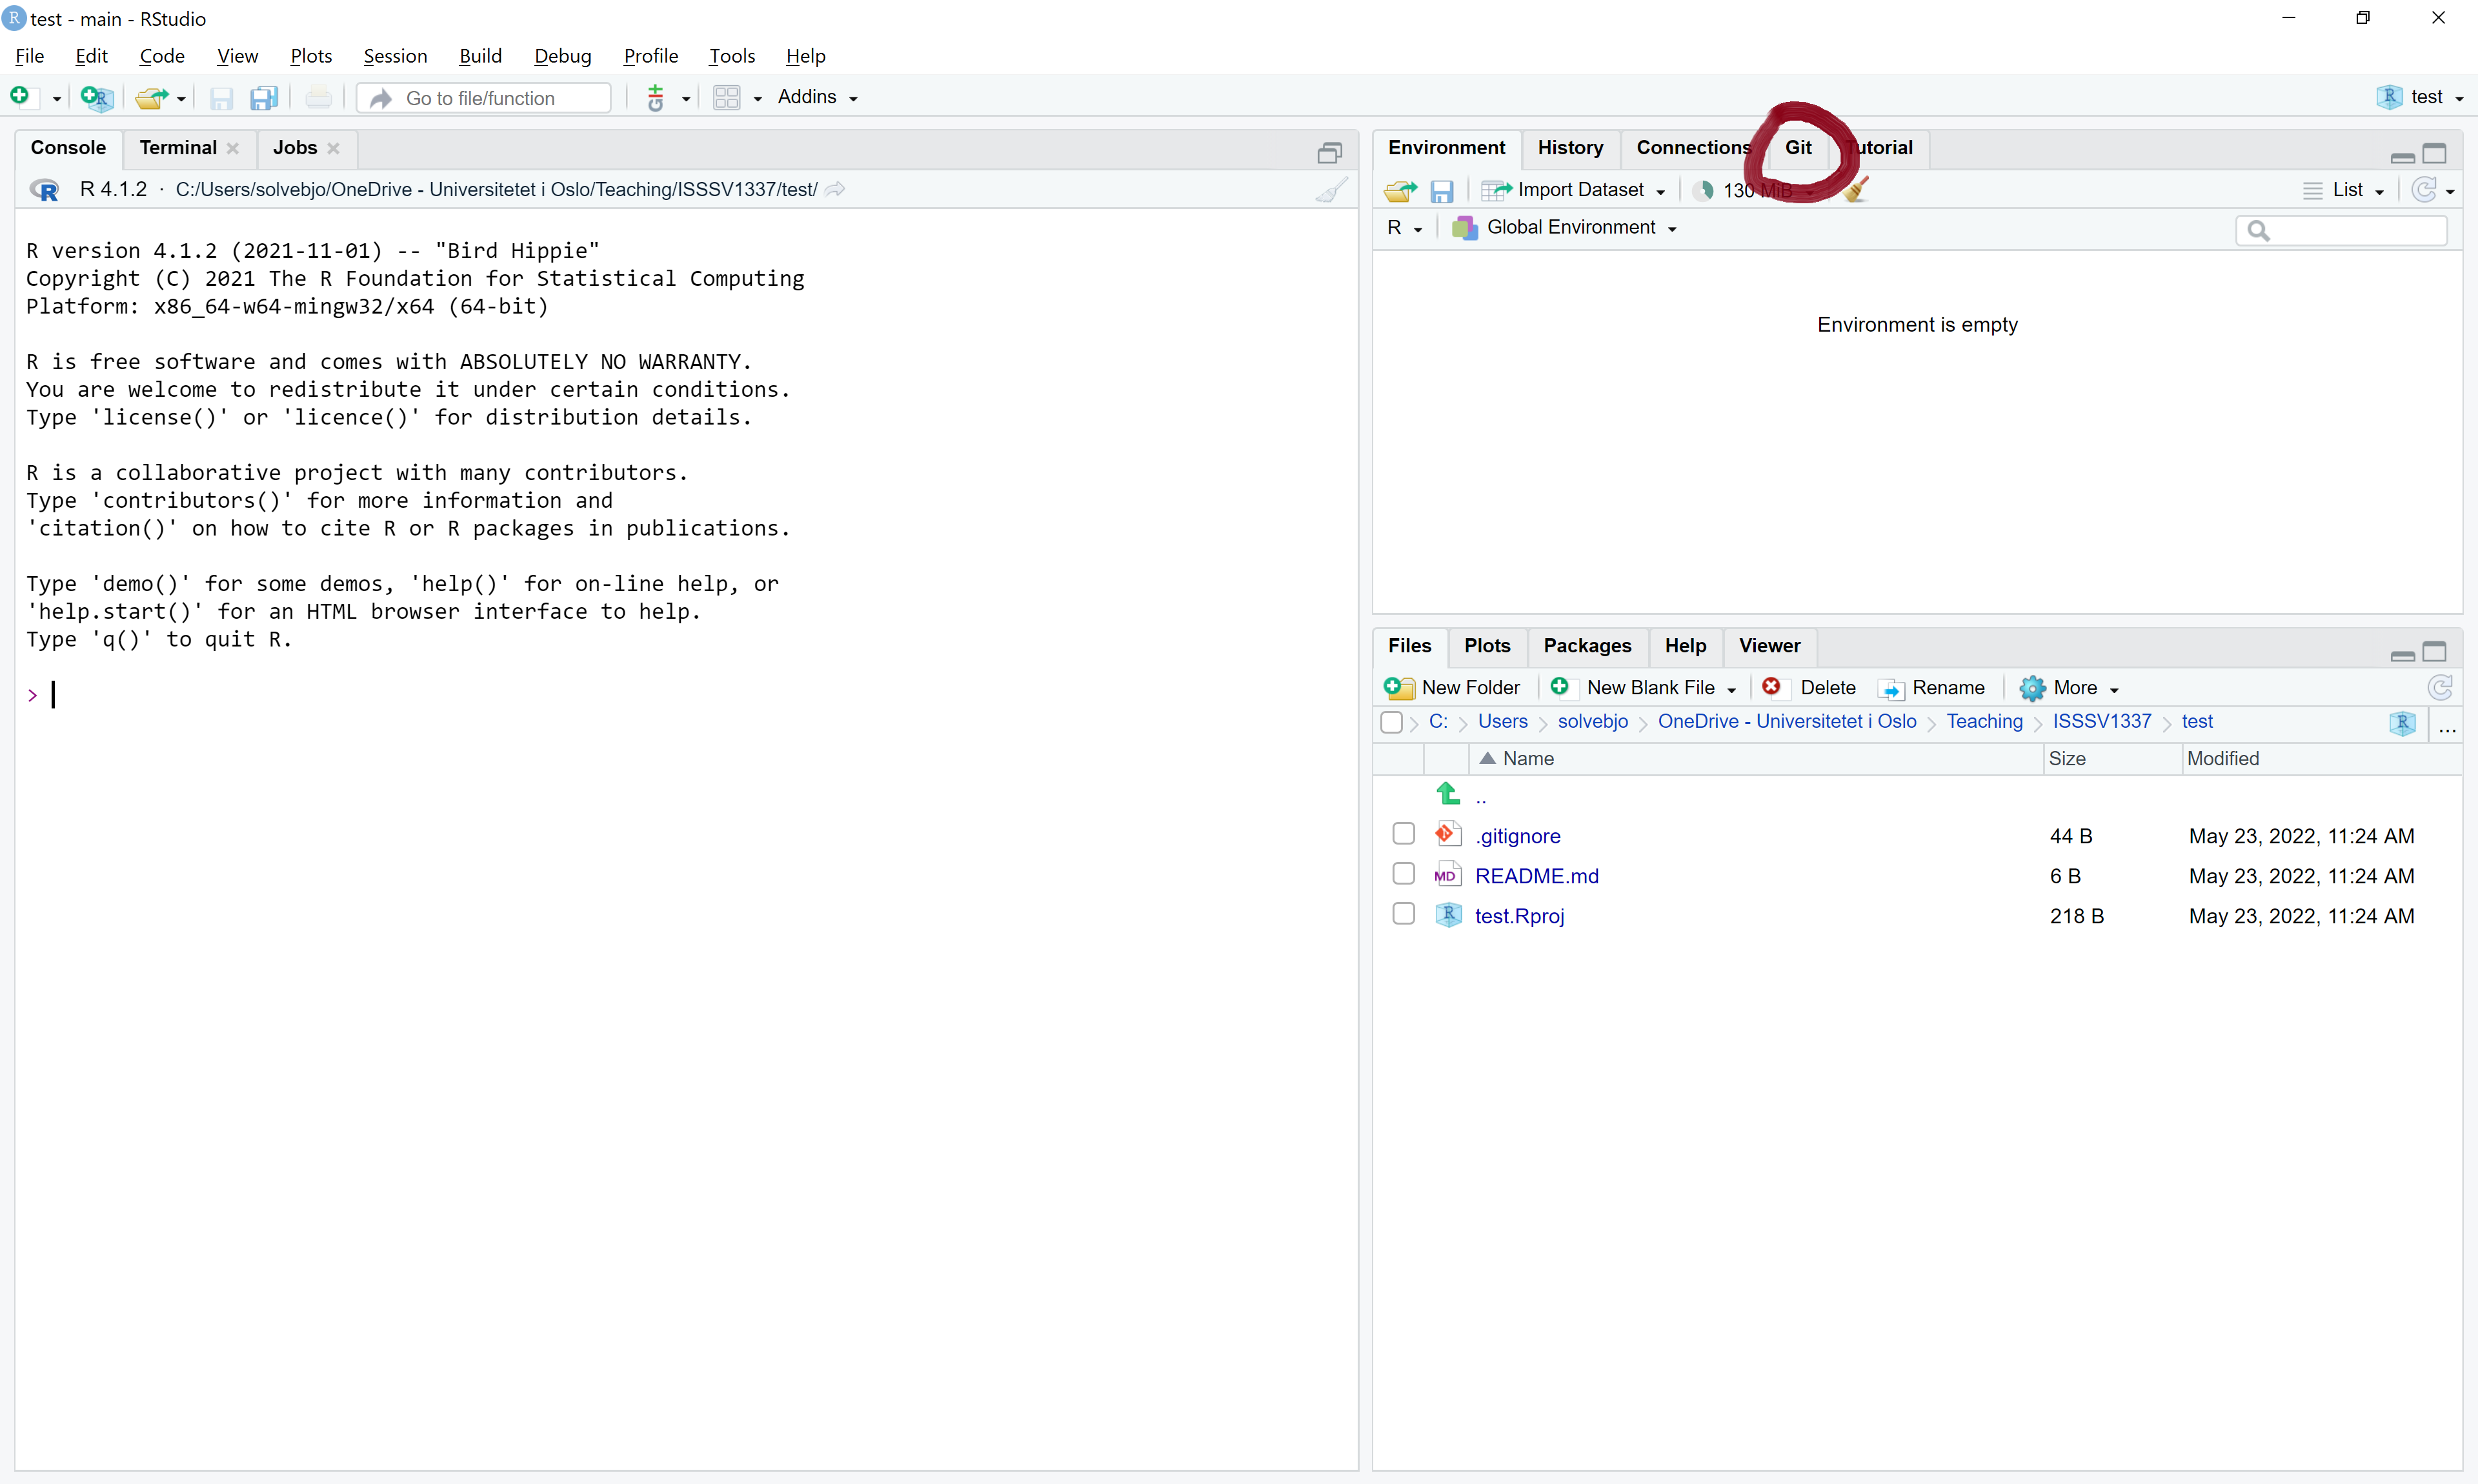
\includegraphics[width=0.8\textwidth,height=\textheight]{./figures/project6.png}

To get the latest updates from your repository, click ``Pull''. Make it
a habit to click ``Pull'' regularly. It will spare you the pain of
so-called ``merge conflicts''. If you want to add your code to the
common repository:

\begin{enumerate}
\def\labelenumi{\arabic{enumi}.}
\tightlist
\item
  Click ``Pull''.
\item
  Click ``Commit''.
\item
  Add a description of what you've done and why.
\item
  Click ``Push''.
\end{enumerate}

\includegraphics[width=0.9\textwidth,height=\textheight]{./figures/githubcommandsrstudio.mp4}

Some of you, if not all, will almost certainly get trouble with Github
during this course. We will deal with them as they arise. Since this is
a learning space which increases the risk of errors, we also recommend
keeping a backup of your repository. This can seem cumbersome, but it's
a part of the learning process. In the end, working with Github will
prove vastly superior to many alternatives, such as sending code over
mail.

\end{document}
